% ESIM – Benutzerhandbuch
% Übersetzen (zweimal, wegen Verzeichnis und Verweisen):
%   cd docs/handbuch && latexmk -pdf handbuch.tex
% oder
%   pdflatex handbuch && pdflatex handbuch
\documentclass[11pt,a4paper,ngerman,parskip=half-,headings=standardclasses,
               toc=bibliography,open=any]{scrbook}

\usepackage[T1]{fontenc}
\usepackage{lmodern}
\usepackage[shorthands=off,ngerman]{babel}
\usepackage{microtype}
\usepackage{amsmath,amssymb}
\usepackage{textcomp}
\usepackage[dvipsnames,table]{xcolor}
\usepackage{graphicx}
\usepackage{booktabs}
\usepackage{tabularx}
\usepackage{longtable}
\usepackage{array}
\usepackage{enumitem}
\usepackage{listings}
\usepackage[most]{tcolorbox}
\usepackage{caption}
\usepackage[hidelinks,pdfusetitle,bookmarksnumbered]{hyperref}

\KOMAoptions{DIV=12}
\makeatletter\renewcommand*{\@pnumwidth}{2.2em}\makeatother
\RedeclareSectionCommand[tocnumwidth=2.2em]{chapter}
\RedeclareSectionCommand[tocindent=2.2em,tocnumwidth=2.9em]{section}
\RedeclareSectionCommand[tocindent=5.1em,tocnumwidth=3.6em]{subsection}
\setkomafont{disposition}{\normalcolor\bfseries}
\setlist{itemsep=0.2ex,topsep=0.4ex}
\captionsetup{font=small,labelfont=bf}
\renewcommand{\arraystretch}{1.15}
\setlength{\emergencystretch}{2em}

\graphicspath{{bilder/}}

% ---------------------------------------------------------------------------
% Farben und Kästen
\definecolor{codebg}{HTML}{F6F6F3}
\definecolor{coderule}{HTML}{C9C8C1}
\definecolor{codestr}{HTML}{1F6F4A}
\definecolor{codekey}{HTML}{1F4F99}
\definecolor{codecom}{HTML}{77766F}
\definecolor{hinweisbg}{HTML}{EEF4FB}
\definecolor{hinweisrule}{HTML}{3987E5}
\definecolor{achtungbg}{HTML}{FBF1E8}
\definecolor{achtungrule}{HTML}{D95926}

\newtcolorbox{hinweis}[1][Hinweis]{enhanced,breakable,colback=hinweisbg,
  colframe=hinweisrule,boxrule=0pt,leftrule=3pt,arc=0pt,outer arc=0pt,
  fonttitle=\bfseries\small,coltitle=hinweisrule!80!black,
  attach title to upper={\ },title={#1:},before skip=1ex,after skip=1ex}
\newtcolorbox{achtung}[1][Achtung]{enhanced,breakable,colback=achtungbg,
  colframe=achtungrule,boxrule=0pt,leftrule=3pt,arc=0pt,outer arc=0pt,
  fonttitle=\bfseries\small,coltitle=achtungrule!80!black,
  attach title to upper={\ },title={#1:},before skip=1ex,after skip=1ex}

% ---------------------------------------------------------------------------
% Quelltext
\lstdefinelanguage{jsonc}{
  morestring=[b]",
  morecomment=[l]{//},
  morecomment=[s]{/*}{*/},
  sensitive=true,
}
\lstdefinelanguage{spice}{
  morecomment=[l]{*},
  morecomment=[l]{;},
  sensitive=false,
}
\lstset{
  basicstyle=\ttfamily\small,
  columns=fullflexible,keepspaces=true,
  backgroundcolor=\color{codebg},
  frame=l,framerule=2pt,rulecolor=\color{coderule},
  xleftmargin=6pt,framexleftmargin=6pt,framesep=4pt,
  aboveskip=1.2ex,belowskip=1.2ex,
  breaklines=true,breakatwhitespace=true,
  postbreak=\mbox{\textcolor{codecom}{$\hookrightarrow$}\space},
  showstringspaces=false,
  upquote=true,
  stringstyle=\color{codestr},
  commentstyle=\color{codecom}\itshape,
  literate=
    {ä}{{\"a}}1 {ö}{{\"o}}1 {ü}{{\"u}}1 {Ä}{{\"A}}1 {Ö}{{\"O}}1 {Ü}{{\"U}}1
    {ß}{{\ss}}1 {µ}{{\textmu}}1 {°}{{\textdegree}}1 {Ω}{{$\Omega$}}1
    {→}{{$\to$}}1 {„}{{\glqq}}1 {“}{{\grqq}}1 {–}{{--}}1 {…}{{\dots}}1
    {·}{{$\cdot$}}1 {²}{{\texttwosuperior}}1 {√}{{$\surd$}}1 {±}{{$\pm$}}1,
}
\lstnewenvironment{json}[1][]{\lstset{language=jsonc,#1}}{}
\lstnewenvironment{shell}[1][]{\lstset{language={},#1}}{}
\lstnewenvironment{spicecode}[1][]{\lstset{language=spice,#1}}{}
\lstnewenvironment{python}[1][]{\lstset{language=Python,
  keywordstyle=\color{codekey},morecomment=[l]{\#},#1}}{}

% ---------------------------------------------------------------------------
% Kurzbefehle
\newcommand{\code}[1]{\texttt{\detokenize{#1}}}         % Quelltext im Fließtext
\DeclareUrlCommand\datei{\urlstyle{tt}}               % Dateinamen (bricht an / und .)
\newcommand{\taste}[1]{{\fboxsep=0.9pt\fboxrule=0.4pt%
  \fbox{\footnotesize\sffamily\vphantom{Ag}\,#1\,}}}    % Taste
\newcommand{\tasten}[2]{\taste{#1}\,+\,\taste{#2}}     % Tastenkombination
\newcommand{\menue}[1]{\textsf{#1}}                     % Menüpunkt
\newcommand{\pfad}{\,$\triangleright$\,}                % Menü › Eintrag
\newcommand{\esim}{\textsf{esim}}
\newcommand{\editor}{\textsf{esim-editor}}
\newcommand{\ohm}{\ensuremath{\Omega}}

\newcolumntype{L}{>{\raggedright\arraybackslash}X}
\newcolumntype{P}[1]{>{\raggedright\arraybackslash}p{#1}}

\hypersetup{pdftitle={ESIM – Benutzerhandbuch},pdfauthor={PhotonPower}}

\begin{document}

\frontmatter
\begin{titlepage}
  \centering
  \vspace*{0.18\textheight}
  {\Huge\bfseries ESIM\par}
  \vspace{1.2ex}
  {\Large Simulator für Schaltungen und differential-algebraische Gleichungen\par}
  \vspace{4ex}
  {\LARGE Benutzerhandbuch\par}
  \vspace{3ex}
  {\large Simulator \esim, Editor \editor, Werkzeuge und Python-Schnittstelle\par}
  \vfill
  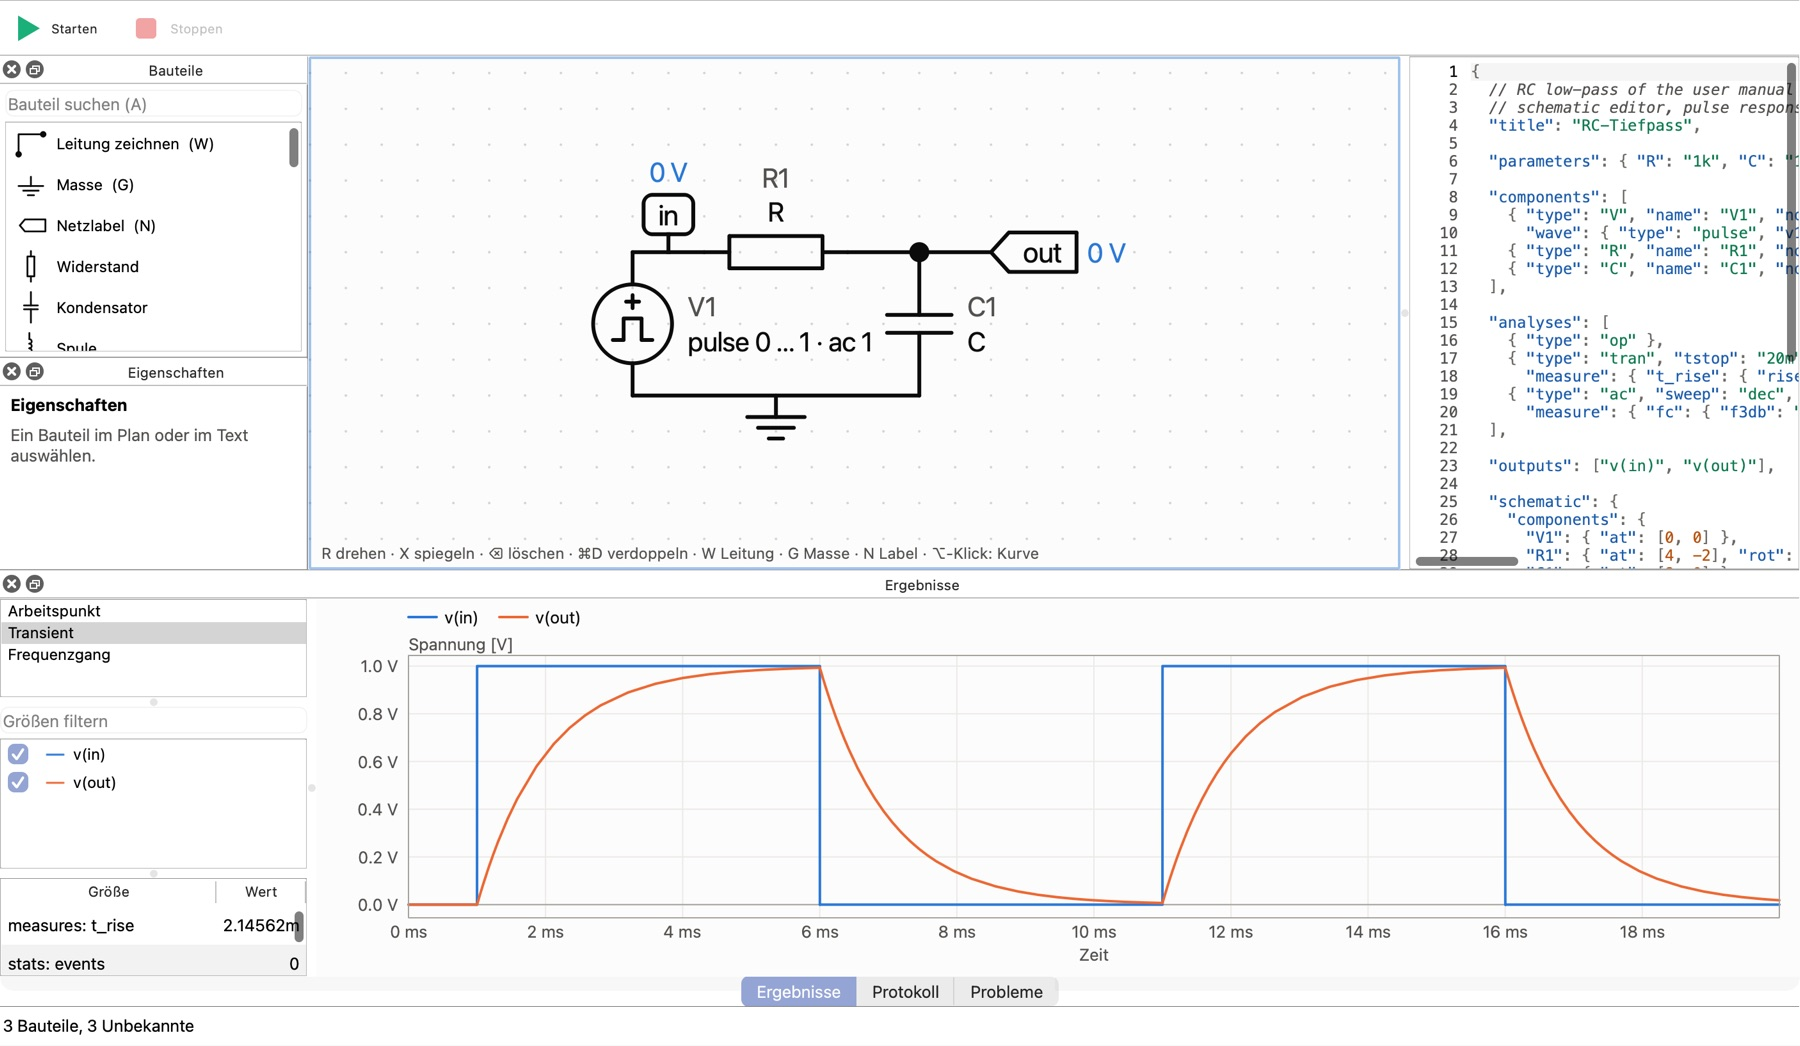
\includegraphics[width=0.9\textwidth]{tiefpass.jpg}\par
  \vfill
  {\large Stand: November 2026\par}
  \vspace{1ex}
  {\small \url{https://github.com/PhotonPower/esim}\quad·\quad Lizenz: MIT\par}
\end{titlepage}

\tableofcontents

\mainmatter

\part{Grundlagen}
\chapter{Einführung}
\label{kap:einfuehrung}

\section{Was ist ESIM?}

ESIM ist ein Simulator für analoge elektronische Schaltungen und für
differential-algebraische Gleichungssysteme (DAE). Er besteht aus
mehreren Teilen, die zusammenarbeiten, aber auch einzeln nutzbar sind:

\begin{description}[style=nextline,leftmargin=2em]
  \item[\esim\ – der Simulator]
    Ein Kommandozeilenprogramm in C++. Es liest eine Eingabedatei im
    JSON-Format, rechnet die darin verlangten Analysen und schreibt die
    Ergebnisse als CSV-Dateien. Der Arbeitspunkt und Messgrößen erscheinen
    zusätzlich auf der Konsole.
  \item[\editor\ – die Oberfläche]
    Ein Programm mit Fenstern (Qt 6) für macOS und Windows: Schaltplan und
    Text nebeneinander, Prüfung der Eingabe beim Tippen, Simulation per
    Tastendruck und ein Kurvenbetrachter mit Zoom, Fadenkreuz,
    Histogrammen und Kennlinienscharen.
  \item[Werkzeuge]
    \datei{tools/spice2json.py} übersetzt SPICE-Netzlisten,
    \datei{tools/plot.py} zeichnet Ergebnisse mit matplotlib, und
    \datei{python/esim.py} ruft den Simulator aus Python auf und liefert die
    Ergebnisse als Datenstrukturen.
\end{description}

\section{Was lässt sich simulieren?}

\begin{itemize}
  \item \textbf{Schaltungen} aus Widerständen, Kondensatoren, Spulen und
    gekoppelten Spulen, unabhängigen und gesteuerten Quellen,
    Verhaltensquellen mit beliebigen Ausdrücken, Dioden,
    Bipolartransistoren (Gummel-Poon), Sperrschicht-FETs, MOSFETs (Level 1,
    EKV, Level 3 und BSIM3v3), idealen Schaltern, idealen Dioden sowie
    verlustlosen und verlustbehafteten Leitungen.
  \item \textbf{Gleichungssysteme}, die direkt in der Eingabedatei stehen:
    gewöhnliche Differentialgleichungen mit algebraischen Nebenbedingungen,
    auch vom Index 3 und höher (sie werden automatisch umgeformt), Vektoren
    von Unbekannten, Totzeiten und Tabellen.
  \item \textbf{Ereignisse}: Umschaltungen und Sprünge, die vom Zustand
    oder von der Zeit abhängen – Schalter, Anschläge, Hysterese, abgetastete
    Regler.
  \item \textbf{Alles gekoppelt} in einem System, etwa eine Schaltung mit
    der Wärmebilanz eines Bauteils und einem digitalen Regler.
\end{itemize}

Die Analysen sind Arbeitspunkt, DC-Sweep, Frequenzgang (AC), Zeitverlauf
(Transient), Rauschen, periodischer stationärer Zustand, Fourier-Analyse,
Empfindlichkeiten und die Anpassung von Parametern an Messdaten. Jede
Analyse lässt sich über Parameter-Sweeps und Monte-Carlo-Läufe wiederholen
und mit Messgrößen (Grenzfrequenz, Anstiegszeit, Effektivwert …)
auswerten.

\section{Das Prinzip}

Der numerische Kern löst allgemein das System
\[
  \frac{d}{dt}\,q(x) + f(x,t) = 0 .
\]
Dabei ist $x$ der Vektor aller Unbekannten (Knotenspannungen, Zweigströme,
Variablen von Gleichungen). Zeilen, in denen $q$ verschwindet, sind
algebraische Bedingungen, alle anderen Differentialgleichungen. Eine
Schaltung liefert $f$ (Ströme) und $q$ (Ladungen und magnetische Flüsse)
über die modifizierte Knotenanalyse, ein Gleichungsblock liefert sie aus dem
Text seiner Gleichungen. Beides landet im selben System; deshalb lassen sich
Schaltung und Gleichungen beliebig koppeln.

Die Ableitungen für das Newton-Verfahren werden für alle Bauteile und alle
Ausdrücke automatisch und exakt gebildet. Sie müssen nirgends von Hand
angegeben werden.

\section{Die Eingabedatei in Kürze}

Eine Simulation ist vollständig durch eine Textdatei beschrieben. Sie ist
JSON mit Kommentaren (\code{//} und \code{/* */}):

\begin{json}
{
  "title": "Einweggleichrichter",

  "models": {
    "DGEN": { "type": "diode", "is": 2.5e-9, "n": 1.75, "cj0": "4p", "tt": "20n" }
  },

  "components": [
    { "type": "V", "name": "V1", "nodes": ["in", "0"],
      "wave": { "type": "sin", "amplitude": 5, "freq": "1k" } },
    { "type": "D", "name": "D1", "nodes": ["in", "out"], "model": "DGEN" },
    { "type": "R", "name": "R1", "nodes": ["out", "0"], "value": "10k" },
    { "type": "C", "name": "C1", "nodes": ["out", "0"], "value": "1u" }
  ],

  "analyses": [
    { "type": "op" },
    { "type": "tran", "tstop": "5m" }
  ],

  "outputs": ["v(in)", "v(out)", "i(V1)"]
}
\end{json}

Die Datei nennt Modelle, Bauteile mit ihren Knoten, die gewünschten
Analysen und die Größen, die ausgegeben werden sollen. Der Editor legt den
Schaltplan in derselben Datei unter dem Schlüssel \code{"schematic"} ab; der
Simulator überliest ihn. Eine im Editor gezeichnete Schaltung lässt sich
also jederzeit auch ohne Editor rechnen.

\section{Über dieses Handbuch}

\begin{description}[style=nextline,leftmargin=2em]
  \item[Teil I – Grundlagen] Installation und ein geführter erster Durchgang
    mit dem Editor.
  \item[Teil II – Der Editor] Alle Fenster, Werkzeuge und Tasten des
    Editors.
  \item[Teil III – Die Eingabedatei] Die vollständige Beschreibung des
    Formats: Zahlen, Ausdrücke, Bauteile, Modelle, Teilschaltungen,
    Analysen, Studien, Gleichungen, Ereignisse und Optionen. Dieser Teil
    gilt für Editor und Kommandozeile gleichermaßen.
  \item[Teil IV – Werkzeuge und Praxis] Kommandozeile, Python, SPICE-Import,
    Fehlersuche und ein Blick auf die Numerik.
  \item[Anhang] Eine vollständige Befehlsreferenz (Programme, alle
    Schlüssel der Eingabedatei mit Standardwerten, Ausdrücke, Befehle des
    Editors), Tastenkürzel, die mitgelieferten Beispiele, eine Kurzreferenz
    und Begriffe.
\end{description}

\paragraph{Schreibweisen.}
Text in \code{Schreibmaschinenschrift} steht so in Dateien oder auf der
Kommandozeile. Menüpunkte sind als \menue{Datei}\pfad\menue{Neu}
geschrieben, Tasten als \taste{R} oder \tasten{Strg}{R}.

\begin{hinweis}[Tasten auf dem Mac]
  Die Kürzel sind in diesem Handbuch in der Windows-Form angegeben. Auf dem
  Mac steht die Befehlstaste (\taste{cmd}) für \taste{Strg}, die Wahltaste
  (\taste{alt}) für \taste{Alt} und die Rückschritttaste für \taste{Entf}.
  Der Editor zeigt in Menüs, Tooltips und der Hinweiszeile jeweils die
  Namen des eigenen Systems.
\end{hinweis}

\chapter{Installation}
\label{kap:installation}

ESIM wird aus dem Quelltext gebaut; für Windows gibt es zusätzlich ein
fertiges Paket aus der automatischen Übersetzung auf GitHub. Der Simulator
\esim\ braucht nur einen C++17-Compiler und CMake, der Editor zusätzlich
Qt~6.

\section{Was gebraucht wird}

\begin{center}
\begin{tabularx}{\textwidth}{@{}lLl@{}}
  \toprule
  Werkzeug & Zweck & nötig für \\
  \midrule
  CMake $\geq$ 3.18 & Build-System & alles \\
  C++17-Compiler & Clang (macOS), MSVC (Windows), GCC (Linux) & alles \\
  Eigen 3, nlohmann/json & Bibliotheken; fehlen sie, lädt CMake sie selbst herunter & alles \\
  Qt $\geq$ 6.5 & Oberfläche des Editors & \editor \\
  Python 3 & Testsuite, Werkzeuge, Python-Schnittstelle & optional \\
  numpy, matplotlib & Ergebnisse als Arrays, Plotten mit \datei{plot.py} & optional \\
  ngspice & drei Vergleichstests gegen ngspice & optional \\
  \bottomrule
\end{tabularx}
\end{center}

Ohne Qt baut CMake nur den Simulator und seine Tests; alles im Teil III
dieses Handbuchs funktioniert dann trotzdem über die Kommandozeile.

\section{macOS}

Mit Homebrew sind alle Voraussetzungen schnell installiert:

\begin{shell}
brew install cmake qt eigen nlohmann-json
\end{shell}

Dann im Ordner des Quelltexts:

\begin{shell}
cmake -S . -B build
cmake --build build --parallel
ctest --test-dir build                 # Tests (optional)
\end{shell}

Der Editor liegt danach als Programmpaket in
\datei{build/editor/esim-editor.app}:

\begin{shell}
open build/editor/esim-editor.app
\end{shell}

Ein eigenständiges Programmpaket, das man in den Ordner »Programme« ziehen
kann (mit den Qt-Bibliotheken, \esim\ und den Beispielen im Paket), legt

\begin{shell}
cmake --install build --prefix dist
\end{shell}

in \datei{dist/esim-editor.app} an.

\begin{hinweis}[Gatekeeper]
  Das Programm ist nicht mit einer Apple-Entwickler-ID signiert. Ein selbst
  gebautes Programm startet ohne Rückfrage. Wird das Paket auf einen
  anderen Mac kopiert, verweigert macOS beim ersten Start unter Umständen das
  Öffnen; dann im Finder mit Rechtsklick \pfad\ \menue{Öffnen} starten oder
  unter \menue{Systemeinstellungen}\pfad\menue{Datenschutz \& Sicherheit}
  einmal erlauben.
\end{hinweis}

\section{Windows 11}

\subsection{Fertiges Paket}

Bei jedem Hochladen auf GitHub baut GitHub Actions ein Windows-Paket. Es
liegt im Repository unter \menue{Actions}, im jeweils neuesten Lauf unter
\menue{Artifacts}, als \datei{esim-windows}. Alternativ mit dem
GitHub-Kommandozeilenprogramm:

\begin{shell}
gh run list --limit 3                    # Nummer des neuesten Laufs
gh run download <Nummer> -n esim-windows
\end{shell}

Das Paket entpacken und \datei{esim-editor.exe} starten. Qt muss dafür nicht
installiert sein; die Qt-Bibliotheken, \datei{esim.exe} und die Beispiele
liegen im selben Ordner. Ein Installationsprogramm gibt es nicht – der
Ordner kann an eine beliebige Stelle kopiert werden.

\begin{hinweis}[SmartScreen]
  Auch unter Windows ist das Programm nicht signiert. Beim ersten Start kann
  SmartScreen warnen; mit \menue{Weitere Informationen}\pfad\menue{Trotzdem
  ausführen} lässt es sich starten.
\end{hinweis}

\subsection{Selbst bauen}

Benötigt werden Visual Studio 2022 oder neuer (oder nur dessen Build Tools)
mit der Arbeitslast »Desktopentwicklung mit C++«, CMake, Git, Qt~6 für MSVC
und optional Python. Mit \code{winget} geht das so:

\begin{shell}
winget install --id Git.Git -e
winget install --id Kitware.CMake -e
winget install --id Python.Python.3.12 -e
winget install --id Microsoft.VisualStudio.2022.BuildTools -e --override "--wait --passive --add Microsoft.VisualStudio.Workload.VCTools --includeRecommended"
python -m pip install aqtinstall
python -m aqt install-qt windows desktop 6.8.3 win64_msvc2022_64 -O C:\Qt
\end{shell}

Dann in einer neuen Eingabeaufforderung im Ordner des Quelltexts:

\begin{shell}
cmake -S . -B build -DCMAKE_PREFIX_PATH=C:/Qt/6.8.3/msvc2022_64
cmake --build build --config Release --parallel
ctest --test-dir build -C Release --output-on-failure
cmake --install build --config Release --prefix dist
\end{shell}

\texttt{dist\textbackslash esim-editor.exe} läuft danach für sich allein.
CMake wählt das neueste installierte Visual Studio von selbst; Qts
Bibliotheken für MSVC 2022 passen auch zu neueren Versionen.

\begin{achtung}[Visual Studio 2026]
  Visual Studio 2026 wird erst von CMake 4.2 an erkannt. Mit einem älteren
  CMake bricht die Konfiguration ab; dann ein neueres CMake installieren
  oder das mit Visual Studio gelieferte verwenden
  (\texttt{Common7\textbackslash\allowbreak IDE\textbackslash CommonExtensions\textbackslash Microsoft\textbackslash CMake\textbackslash CMake\textbackslash bin}).
\end{achtung}

Alle Programme arbeiten intern mit UTF-8; Dateien und Ordner mit Umlauten
(etwa \texttt{C:\textbackslash\allowbreak Übung\textbackslash\allowbreak Schaltkreis~ä.json}) sind kein Problem.

\section{Linux}

Der Simulator und der Editor bauen auch mit GCC unter Linux; ein Paket wird
dafür nicht gepflegt. Mit den Paketen der Distribution (z.\,B. unter Debian
und Ubuntu \code{cmake g++ qt6-base-dev libeigen3-dev nlohmann-json3-dev})
genügen dieselben Befehle wie unter macOS.

\section{Optionale Teile}

\paragraph{Python.}
Die Python-Schnittstelle (Kapitel~\ref{kap:python}) braucht nur die
Standardbibliothek. Mit \code{pip install numpy matplotlib} liefert sie
numpy-Arrays, und \datei{tools/plot.py} kann zeichnen.

\paragraph{ngspice.}
Ist ngspice installiert (unter Windows \datei{ngspice_con.exe} im Suchpfad),
legt CMake drei zusätzliche Tests an, die esims Modelle (BSIM3, MOS Level~3,
SPICE-Teilschaltungen) gegen ngspice vergleichen. Für die Benutzung ist
ngspice nicht nötig.

\section{Prüfen, ob alles läuft}

\begin{shell}
./build/esim examples/rc_lowpass.json -o results
\end{shell}

Auf der Konsole erscheinen der Arbeitspunkt und eine Zeile je Analyse; die
Kurven liegen danach in \datei{results/rc_lowpass.ac.csv} und
\datei{results/rc_lowpass.tran.csv}. Im Editor öffnet
\menue{Datei}\pfad\menue{Beispiele} dieselbe Datei; \tasten{Strg}{R} rechnet
sie.

\chapter{Erste Schritte}
\label{kap:erste-schritte}

Dieses Kapitel führt einmal durch die wichtigsten Arbeitsschritte: eine
Schaltung anlegen, simulieren, Werte ändern, einen Frequenzgang mit
Grenzfrequenz bestimmen, im Plan zeichnen und eine Parameterstudie rechnen.
Am Ende steht dieselbe Simulation einmal auf der Kommandozeile. Wer die
Schritte nachvollzieht, kennt danach den Großteil der täglichen Arbeit.

\section{Eine neue Schaltung}

Nach dem Start zeigt der Editor ein leeres Fenster.
\menue{Datei}\pfad\menue{Neu} (\tasten{Strg}{N}) legt eine Vorlage an: einen
RC-Tiefpass aus einer Pulsquelle \code{V1}, einem Widerstand \code{R1} und
einem Kondensator \code{C1}.

Das Fenster hat drei große Bereiche (Abbildung~\ref{abb:tiefpass}):

\begin{itemize}
  \item in der Mitte der \textbf{Schaltplan},
  \item rechts der \textbf{Text} der Datei, also die Eingabe für den
    Simulator,
  \item unten die \textbf{Ergebnisse}, daneben als Reiter das
    \textbf{Protokoll} und die Liste der \textbf{Probleme},
  \item links die Listen \textbf{Bauteile} und \textbf{Eigenschaften}.
\end{itemize}

\begin{figure}[htbp]
  \centering
  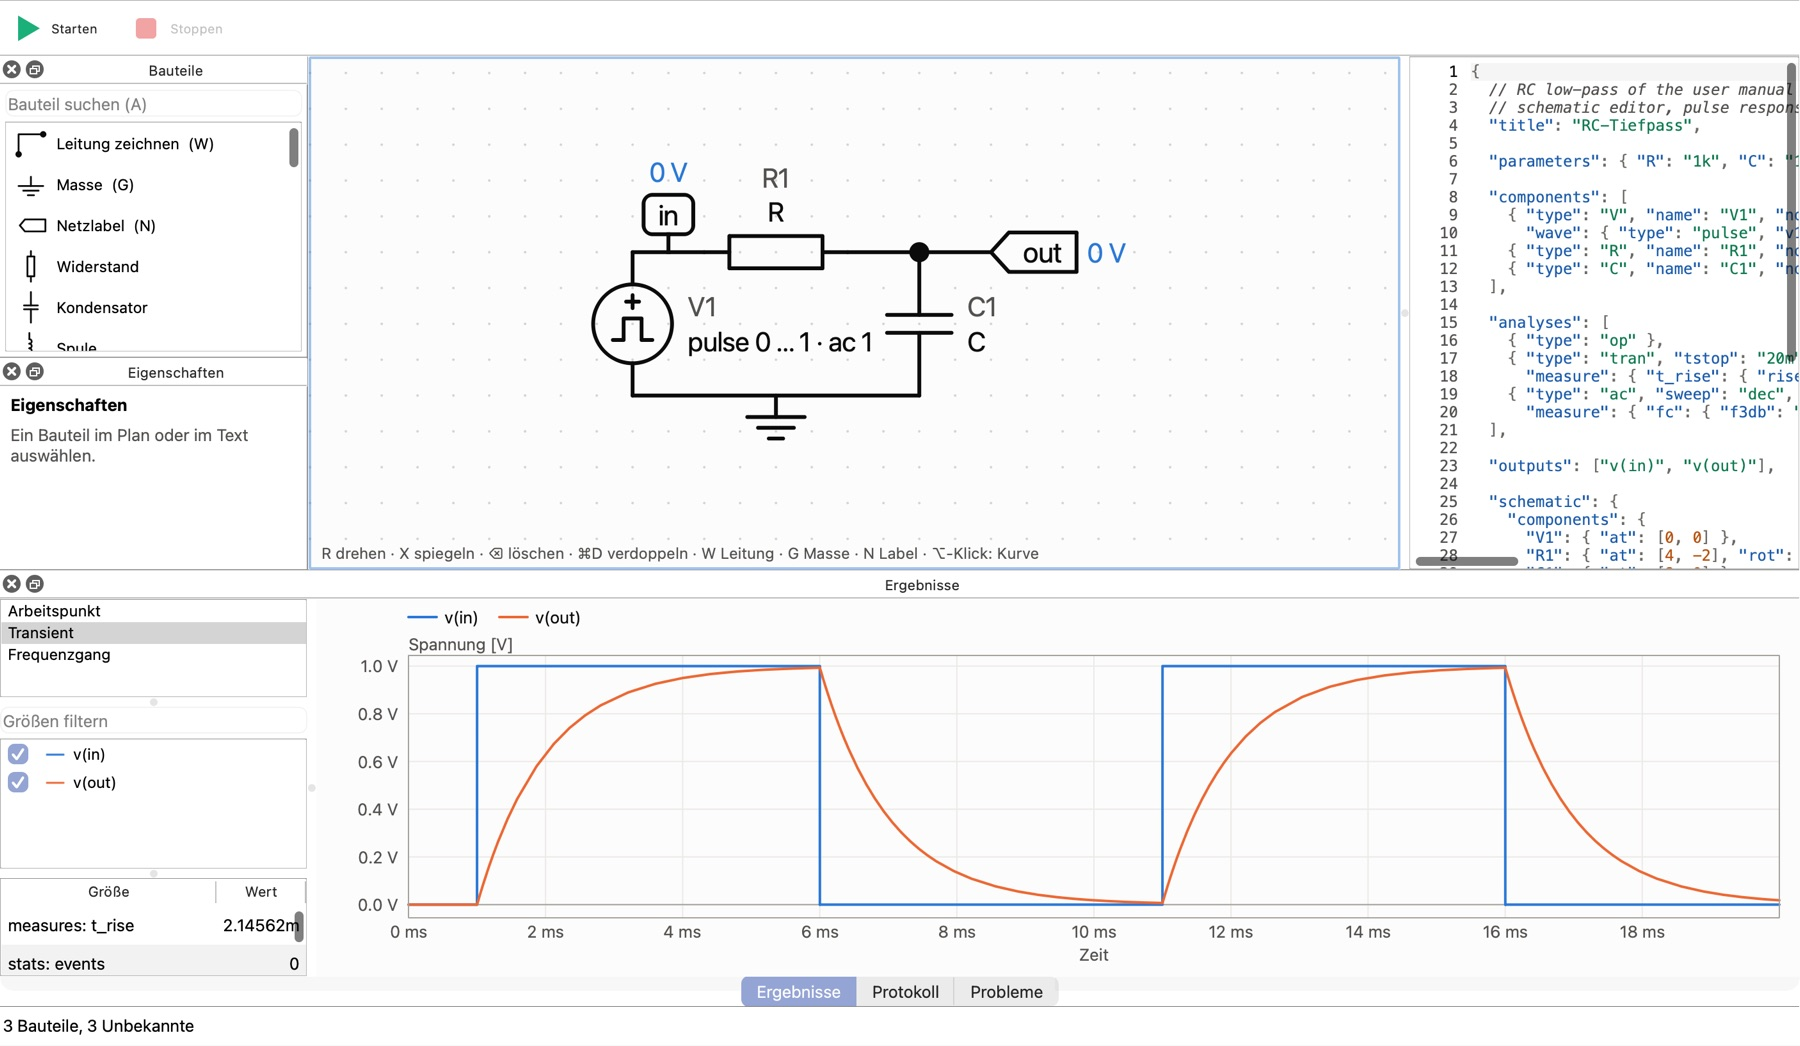
\includegraphics[width=\textwidth]{tiefpass.jpg}
  \caption{Der RC-Tiefpass im Editor: Plan, Text und Sprungantwort. Die
    Datei liegt als \code{docs/handbuch/tiefpass.json} bei.}
  \label{abb:tiefpass}
\end{figure}

Plan und Text sind zwei Ansichten derselben Datei. Ein Klick auf \code{R1}
im Plan markiert dessen Zeile im Text; setzt man den Textcursor in die
Zeile von \code{C1}, wird \code{C1} im Plan ausgewählt. Jede Änderung im
Plan erscheint sofort im Text und umgekehrt.

\section{Die erste Simulation}

\menue{Simulation}\pfad\menue{Starten} oder \tasten{Strg}{R} startet die
Rechnung. Der Simulator liest die Datei von der Platte; deshalb sichert der
Editor vorher ungesicherte Änderungen, und eine Datei ohne Namen fragt nach
einem Speicherort. Während der Rechnung zeigt
die Statuszeile den Fortschritt; \tasten{Strg}{.} bricht ab.

Danach steht im Ergebnisfeld links die Liste der Analysen der Datei:
\menue{Arbeitspunkt} und \menue{Transient}. Ein Klick auf
\menue{Transient} zeigt den Zeitverlauf: die Pulsspannung \code{v(in)} und
die Kondensatorspannung \code{v(out)}, die mit der Zeitkonstante
$\tau = RC = 1\,\text{ms}$ folgt. Mit den Häkchen unter \menue{Größen
filtern} werden Kurven ein- und ausgeblendet.

Im Kurvenfeld:
\begin{itemize}
  \item Mausrad oder Spreizen auf dem Touchpad zoomt in $x$, mit
    \taste{Strg} in $y$,
  \item Ziehen mit der Maus zoomt auf ein Rechteck,
  \item Doppelklick (oder \tasten{Strg}{0}) zeigt wieder alles,
  \item das Fadenkreuz folgt der Maus und zeigt die Werte aller Kurven.
\end{itemize}

Im Plan stehen jetzt an den Netzlabels die Spannungen des Arbeitspunkts
(hier 0\,V, weil die Pulsquelle bei $t=0$ auf 0\,V steht).

\section{Werte ändern}

Ein Klick auf \code{R1} zeigt unter \menue{Eigenschaften} ein Formular mit
Name, Anschlüssen und allen Werten des Bauteils. Dort \code{value} auf
\code{2.2k} setzen und mit der Eingabetaste bestätigen. Im Text steht
sofort \code{"value": "2.2k"}. Nach \tasten{Strg}{R} steigt \code{v(out)}
deutlich langsamer.

Genauso gut lässt sich der Wert direkt im Text ändern. Der Editor prüft
die Datei beim Tippen mit dem Parser des Simulators: Ein Tippfehler wie
\code{"valeu"} erscheint sofort als Warnung an der Zeile und in der Liste
\menue{Probleme}; ein Doppelklick dort springt an die Stelle.

\begin{hinweis}
  Zahlen dürfen SI-Präfixe tragen: \code{2.2k}, \code{100n}, \code{4.7meg}.
  Groß- und Kleinschreibung zählt – \code{M} ist Mega, \code{m} Milli
  (Abschnitt~\ref{sec:zahlen}).
\end{hinweis}

\section{Frequenzgang und Grenzfrequenz}

Für einen Frequenzgang braucht die Quelle eine Kleinsignalamplitude und die
Datei eine AC-Analyse. In den Eigenschaften von \code{V1} in der letzten
Zeile \menue{Neu} den Namen \code{ac} und den Wert \code{1} eintragen und
mit \taste{+} übernehmen. Dann im Text unter \code{"analyses"} eine Zeile
ergänzen:

\begin{json}
"analyses": [
  { "type": "op" },
  { "type": "tran", "tstop": "20m" },
  { "type": "ac", "sweep": "dec", "points": 20, "fstart": 1, "fstop": "100k",
    "measure": { "fc": { "f3db": "v(out)" } } }
],
\end{json}

Nach \tasten{Strg}{R} zeigt \menue{Frequenzgang} Betrag (in dB) und Phase
über der Frequenz. Die Messgröße \code{fc} steht in der Wertetabelle unter
der Liste der Größen: rund 159\,Hz für 1\,k\ohm\ und 1\,µF, wie
$f_c = 1/(2\pi RC)$ erwarten lässt.

\section{Im Plan zeichnen}

Nun soll eine zweite RC-Stufe an \code{out} angehängt werden.

\begin{enumerate}
  \item \textbf{Widerstand platzieren.} \taste{A} drücken (oder in die
    Liste \menue{Bauteile} klicken), »wid« tippen, Eingabetaste. Am
    Mauszeiger hängt jetzt ein Widerstand. \taste{R} dreht ihn um 90°,
    \taste{X} spiegelt ihn. Ein Klick setzt ihn ab; der nächste Klick setzt
    einen weiteren. \taste{Esc} beendet das Platzieren.
  \item \textbf{Kondensator platzieren} auf dieselbe Weise (»kon«).
  \item \textbf{Leitungen ziehen.} \taste{W} startet eine Leitung. Ein Klick
    setzt den Anfang, jeder weitere Klick eine Ecke. Die Leitung knickt
    rechtwinklig; \taste{/} wählt, ob sie zuerst waagrecht oder zuerst
    senkrecht verläuft. Sie endet von selbst, sobald ein Klick einen
    Anschluss oder eine andere Leitung trifft; sonst beendet ein Doppelklick
    oder \taste{Esc} sie. \taste{Entf} nimmt die letzte Ecke zurück.
  \item \textbf{Masse.} \taste{G} hängt ein Massesymbol an den Mauszeiger;
    ein Klick auf das freie Ende des Kondensators setzt es.
  \item \textbf{Netzlabel.} \taste{N} fragt nach einem Namen, z.\,B.
    \code{out2}, und setzt das Label per Klick an die neue Leitung.
\end{enumerate}

Der Text enthält danach zwei neue Bauteile \code{R2} und \code{C2} mit den
Knoten, die der Plan vorgibt: \code{["out", "out2"]} und
\code{["out2", "0"]}. Knotennamen entstehen aus den Labels; Netze ohne Label
bekommen Namen wie \code{n1}. Wer \code{v(out2)} als Kurve sehen will,
ergänzt es unter \code{"outputs"} – oder klickt nach der Simulation mit
gedrückter \taste{Alt}-Taste auf die Leitung.

\begin{hinweis}[Alt-Klick]
  Ein Klick mit \taste{Alt} auf eine Leitung zeigt deren Spannung, auf ein
  Bauteil dessen Strom als Kurve. Ist die Größe nicht unter
  \code{"outputs"} gespeichert, sagt die Statuszeile, was einzutragen ist.
\end{hinweis}

Ausgewählte Bauteile verschiebt man durch Ziehen oder mit den Pfeiltasten
(mit \taste{Umschalt} in Fünferschritten); angeschlossene Leitungen gehen
mit. \tasten{Strg}{D} verdoppelt die Auswahl, \taste{Entf} löscht sie,
\tasten{Strg}{Z} nimmt jeden Schritt zurück – auch Änderungen im Text,
denn Plan und Text haben eine gemeinsame Undo-Geschichte.

\section{Parameter und eine Parameterstudie}

Statt fester Werte können Bauteile Parameter verwenden. Im Text:

\begin{json}
"parameters": { "R": "1k", "C": "1u" },
"components": [
  ...
  { "type": "R", "name": "R1", "nodes": ["in", "out"], "value": "R" },
  { "type": "C", "name": "C1", "nodes": ["out", "0"], "value": "C" }
],
\end{json}

Eine Analyse lässt sich nun für mehrere Werte eines Parameters wiederholen:

\begin{json}
{ "type": "tran", "tstop": "20m",
  "param_sweep": { "param": "C", "values": ["470n", "1u", "2.2u"] } }
\end{json}

Das Ergebnis zeigt eine Kurvenschar: eine Farbstufe je Wert. Messgrößen
einer Studie lassen sich zusätzlich als Kennlinie über dem Parameter
darstellen (Kapitel~\ref{kap:editor-ergebnisse}).

\section{Sichern und auf der Kommandozeile rechnen}

\tasten{Strg}{S} sichert die Datei. Sie enthält alles: Bauteile, Modelle,
Analysen und unter \code{"schematic"} den Plan. Dieselbe Datei rechnet der
Simulator ohne Editor:

\begin{shell}
esim tiefpass.json -o ergebnisse
\end{shell}

\begin{shell}
RC-Tiefpass
3 components, 3 unknowns (2 node voltages, 1 branch currents, 0 equation variables)
[op] converged after 1 iterations (newton)
  v(in)  = 0
  v(out) = 0
[tran] 0 .. 0.02 s, bdf (order up to 5): 160 steps ... -> ergebnisse/tiefpass.tran.csv
  t_rise = 0.00214562
[ac] 1 .. 100000 Hz: 101 points -> ergebnisse/tiefpass.ac.csv
  fc = 159.182
\end{shell}

Die Kurven liegen als CSV-Dateien im Ordner \datei{ergebnisse}, eine je
Analyse. Wie es von hier weitergeht, beschreiben Teil~II (Editor) und
Teil~III (alle Möglichkeiten der Eingabedatei).


\part{Der Editor}
\chapter{Das Hauptfenster}
\label{kap:editor-fenster}

\section{Aufbau}

Das Hauptfenster besteht aus einem festen Mittelteil und mehreren Feldern,
die sich verschieben, abtrennen und ausblenden lassen:

\begin{center}
\begin{tabularx}{\textwidth}{@{}lL@{}}
  \toprule
  Bereich & Inhalt \\
  \midrule
  Schaltplan (Mitte) & Zeichenfläche für die Schaltung oder eine
    Teilschaltung; darüber bei Teilschaltungen eine Leiste mit dem Weg
    zurück zur Hauptschaltung, darunter eine Hinweiszeile mit den Tasten des
    gerade aktiven Werkzeugs. \\
  Text (rechts) & Die Eingabedatei mit Hervorhebung, Zeilennummern und
    Einrückung. \\
  Bauteile & Liste aller Bauteile, Werkzeuge, Teilschaltungen der Datei und
    der Modelle der Bibliothek; mit Suchfeld. \\
  Eigenschaften & Formular für das ausgewählte Bauteil. \\
  Ergebnisse & Analysen, Größen, Wertetabelle und Kurven der letzten
    Simulation. \\
  Protokoll & Ausgabe des Simulators: Fortschritt, Meldungen, Warnungen und
    Fehler, farbig hervorgehoben. \\
  Probleme & Fehler und Warnungen der Prüfung beim Tippen und
    Widersprüche zwischen Plan und Text; Doppelklick springt zur Zeile. \\
  \bottomrule
\end{tabularx}
\end{center}

Die Felder werden an ihrer Titelleiste gezogen. Lässt man eines über einem
anderen los, werden beide zu Reitern; zieht man es aus dem Fenster heraus,
schwebt es frei. \menue{Ansicht} blendet jedes Feld ein und aus. Lage und
Größe aller Felder, die zuletzt geöffneten Dateien und die Einstellungen der
Bibliothek merkt sich der Editor über den Neustart hinweg.

\section{Menüs}

\subsection*{Datei}
\begin{tabularx}{\textwidth}{@{}lP{3.5cm}L@{}}
  \toprule
  Eintrag & Kürzel & Wirkung \\
  \midrule
  Neu & \tasten{Strg}{N} & Neue Datei aus einer Vorlage (RC-Tiefpass mit Plan). \\
  Öffnen \dots & \tasten{Strg}{O} & Eine \datei{.json}-Datei öffnen. \\
  Zuletzt geöffnet & & Die letzten zehn Dateien; \menue{Liste leeren}. \\
  Beispiele & & Die mitgelieferten Beispiele (Anhang~\ref{sec:beispiele}). \\
  Sichern & \tasten{Strg}{S} & Datei sichern. \\
  Sichern unter \dots & \tasten{Umschalt+Strg}{S} & Unter neuem Namen sichern. \\
  Beenden & \tasten{Strg}{Q} & Fragt bei ungesicherten Änderungen nach. \\
  \bottomrule
\end{tabularx}

Eine Datei lässt sich auch beim Start übergeben
(\code{esim-editor datei.json}); unter Windows genügt es, sie auf
\datei{esim-editor.exe} zu ziehen, unter macOS auf das Programmsymbol im
Dock oder über \menue{Öffnen mit}.

\subsection*{Bearbeiten}
\begin{tabularx}{\textwidth}{@{}lP{3.5cm}L@{}}
  \toprule
  Eintrag & Kürzel & Wirkung \\
  \midrule
  Widerrufen / Wiederholen & \tasten{Strg}{Z} / \tasten{Strg}{Y} & Gemeinsam für Plan und Text. \\
  Ausschneiden, Kopieren, Einfügen & \tasten{Strg}{X}, \dots{} & Im Text. \\
  Alles auswählen & \tasten{Strg}{A} & Im Text. \\
  Kommentar ein/aus & \tasten{Strg}{/} & Markierte Zeilen mit \code{//} aus- und einkommentieren. \\
  Auswahl in Teilschaltung umwandeln \dots & \tasten{Strg}{G} & Siehe Abschnitt~\ref{sec:auslagern}. \\
  Modellbibliothek \dots & \tasten{Strg}{L} & Siehe Kapitel~\ref{kap:editor-bibliothek}. \\
  \bottomrule
\end{tabularx}

Unter macOS heißt \menue{Wiederholen} \tasten{Umschalt+cmd}{Z}.

\subsection*{Simulation}
\begin{tabularx}{\textwidth}{@{}lP{3.5cm}L@{}}
  \toprule
  Eintrag & Kürzel & Wirkung \\
  \midrule
  Starten & \tasten{Strg}{R} & Sichert und rechnet die Datei. \\
  Stoppen & \tasten{Strg}{.} & Bricht die laufende Simulation ab. \\
  \bottomrule
\end{tabularx}

Beide Befehle stehen auch in der Werkzeugleiste oben.

\subsection*{Ansicht}
\begin{tabularx}{\textwidth}{@{}lP{3.5cm}L@{}}
  \toprule
  Eintrag & Kürzel & Wirkung \\
  \midrule
  Schaltplan, Text & & Plan oder Text ausblenden (eines bleibt immer sichtbar). \\
  Schaltplan einpassen & \taste{F} im Plan & Ganze Schaltung zeigen. \\
  Bauteile, Eigenschaften, \dots & & Felder ein- und ausblenden. \\
  Kurven: alles zeigen & \tasten{Strg}{0} & Zoom der Kurven zurücksetzen. \\
  \bottomrule
\end{tabularx}

\section{Statuszeile}

Die Statuszeile am unteren Rand zeigt nach jeder Prüfung eine kurze
Zusammenfassung (»3 Bauteile, 3 Unbekannte«) oder die Zahl der Fehler und
Warnungen, während einer Simulation den Fortschritt der laufenden Analyse
in Prozent und danach die Rechenzeit. Auch Rückmeldungen auf Aktionen
(»„NPN\_GEN“ in die Datei übernommen«) erscheinen dort.

\section{Wie der Editor rechnet}

Der Editor startet für jede Simulation das Programm \esim\ als eigenen
Prozess, mit einem temporären Ordner für die Ergebnisse. Das hat zwei
Vorteile: Ein Absturz oder eine Endlosschleife des Simulators trifft nicht
den Editor, und \menue{Stoppen} beendet einfach den Prozess. \esim\ liegt im
Programmpaket neben dem Editor.

Die Prüfung beim Tippen läuft dagegen im Editor selbst, mit demselben
Parser wie der Simulator, in einem Hintergrund-Thread und kurz verzögert,
damit sie das Tippen nicht bremst. Was sie meldet, meldet auch der
Simulator.

\section{Start mit Optionen}

\begin{shell}
esim-editor [datei.json] [--subcircuit <name>] [--run] [--snapshot <bild.png>]
\end{shell}

\begin{tabularx}{\textwidth}{@{}lL@{}}
  \toprule
  Option & Wirkung \\
  \midrule
  \code{datei.json} & Öffnet die Datei. \\
  \code{--subcircuit name} & Zeigt den Plan der Teilschaltung \code{name}. \\
  \code{--run} & Startet gleich die Simulation. \\
  \code{--snapshot bild.png} & Sichert das Fenster (nach der Simulation) als Bild und beendet sich. Gedacht für Dokumentation und Tests; alle Bildschirmfotos dieses Handbuchs sind so entstanden. \\
  \bottomrule
\end{tabularx}

Unter macOS liegt das Programm im Paket:

\begin{shell}
esim-editor.app/Contents/MacOS/esim-editor
\end{shell}

\section{Hell und dunkel}

Der Editor folgt der Darstellung des Betriebssystems. Plan, Kurven und
Symbole haben für den hellen und den dunklen Modus eigene, aufeinander
abgestimmte Farben. Die acht Kurvenfarben sind so gewählt, dass sie auch bei
Farbfehlsichtigkeit unterscheidbar bleiben; Kurvenscharen aus
Parameterstudien erscheinen als Stufen einer Blauskala.

\chapter{Der Schaltplan}
\label{kap:editor-schaltplan}

\section{Grundsätzliches: Plan und Text}

Der Text der Datei ist maßgeblich; der Plan ist eine zweite Ansicht davon.
Nach jeder Textänderung liest der Editor die Datei neu und baut den Plan
auf: Bauteile und ihre Knoten kommen aus \code{"components"}, Lage,
Leitungen, Labels und Masse aus \code{"schematic"}. Umgekehrt schreibt jede
Änderung im Plan nur die betroffenen Stellen des Texts – Name und
\code{"nodes"} geänderter Bauteile, neue und gelöschte Bauteile und den
Abschnitt \code{"schematic"}. Kommentare, Reihenfolge und Formatierung der
Datei bleiben erhalten, und jede Änderung im Plan ist genau ein Schritt der
gemeinsamen Undo-Geschichte.

Was sich nicht zeichnen lässt – Gleichungen, Ereignisse, Analysen,
Optionen – bleibt im Text. Bauteile ohne Symbol im Plan (etwa die Kopplung
\code{K}) erscheinen trotzdem und lassen sich wie alle anderen auswählen.

\begin{hinweis}[Dateien ohne Plan]
  Öffnet man eine Datei ohne \code{"schematic"}, ordnet der Editor die
  Bauteile in Zeilen an und setzt an jeden Anschluss ein Netzlabel mit dem
  Knotennamen aus dem Text. Die Schaltung ist damit vollständig und richtig
  verbunden, nur noch nicht schön gezeichnet. Sobald man im Plan etwas
  ändert, schreibt der Editor den Abschnitt \code{"schematic"} in die Datei.
\end{hinweis}

\section{Ansicht: verschieben und zoomen}

\begin{center}
\begin{tabularx}{\textwidth}{@{}P{5.2cm}L@{}}
  \toprule
  Bedienung & Wirkung \\
  \midrule
  Mausrad & Zoomt um den Mauszeiger. \\
  \taste{Strg} + Mausrad & Zoomt (auch auf dem Touchpad). \\
  Touchpad: wischen mit zwei Fingern & Verschiebt die Ansicht. \\
  Touchpad: spreizen & Zoomt. \\
  Touchpad: zweimal tippen mit zwei Fingern (macOS) & Zeigt alles. \\
  mittlere Maustaste ziehen & Verschiebt die Ansicht. \\
  \taste{Leertaste} halten und ziehen & Verschiebt die Ansicht. \\
  \taste{F} & Zeigt die ganze Schaltung. \\
  \bottomrule
\end{tabularx}
\end{center}

Fährt die Maus über einen Anschluss oder eine Leitung, nennt ein Tooltip
den Knoten (»Knoten „out“«, »Masse«) und nach einer Simulation seine
Spannung im Arbeitspunkt. Alle Leitungen desselben Netzes werden dabei
hervorgehoben.

\section{Auswählen}

\begin{itemize}
  \item \textbf{Klick} auf ein Bauteil, eine Leitung, ein Label oder eine
    Masse wählt es aus; ein Klick ins Leere hebt die Auswahl auf.
  \item \textbf{Umschalt-Klick} fügt hinzu oder nimmt wieder heraus.
  \item \textbf{Rechteck aufziehen} (im Leeren beginnen) wählt alles darin;
    mit \taste{Umschalt} kommt es zur bisherigen Auswahl hinzu.
\end{itemize}

Ein einzelnes ausgewähltes Bauteil wird im Text markiert, und
\menue{Eigenschaften} zeigt sein Formular. Umgekehrt wählt der Plan das
Bauteil aus, in dessen Text der Cursor steht.

\section{Bauteile platzieren}

Bauteile kommen aus der Liste \menue{Bauteile}:
\begin{itemize}
  \item \taste{A} im Plan setzt den Cursor ins Suchfeld der Liste. Ein paar
    Buchstaben genügen (»kon«, »npn«, »puls«); die Eingabetaste nimmt den
    ersten Treffer.
  \item Ein Klick auf einen Eintrag der Liste wählt ihn ebenso.
\end{itemize}

Danach hängt das Bauteil am Mauszeiger. \taste{R} dreht es um 90° im
Uhrzeigersinn, \taste{X} spiegelt es; ein Klick setzt es ab. Das Werkzeug
bleibt aktiv, damit man gleich weitere setzen kann – jedes bekommt den
nächsten freien Namen (\code{R1}, \code{R2}, \dots). \taste{Esc} oder ein
Rechtsklick beendet das Platzieren.

Die Liste enthält:

\begin{center}
\begin{tabularx}{\textwidth}{@{}lL@{}}
  \toprule
  Eintrag & Vorgabe im Text \\
  \midrule
  Widerstand, Kondensator, Spule & \code{"value": "1k"}, \code{"1u"}, \code{"1m"} \\
  Spannungsquelle & \code{"dc": 1} \\
  Sinusquelle & \code{"dc": 0, "ac": 1}, Sinus 1\,V, 1\,kHz \\
  Pulsquelle & Puls 0 \dots 1\,V, Periode 1\,ms \\
  Stromquelle & \code{"dc": "1m"} \\
  Diode, Ideale Diode & ohne Modell bzw. \code{"vf": 0.7} \\
  NPN, PNP, N-MOSFET, P-MOSFET, N-JFET, P-JFET & ohne Modell (Standardwerte von SPICE) \\
  Spannungs-/stromgesteuerte Quellen E, G, F, H & Verstärkung 1 bzw. \code{"control": "V1"} \\
  Verhaltensquelle, Spannung / Strom & \code{"v": "0"} bzw. \code{"i": "0"} \\
  Schalter, spannungsgesteuert & \code{"vt": 0.5} \\
  Leitung & \code{"z0": 50, "td": "1n"} \\
  Kopplung zweier Spulen & \code{"inductors": ["L1", "L2"], "k": 0.99} \\
  Teilschaltung »\textit{name}« & je Teilschaltung der Datei ein Eintrag \\
  Modelle der Bibliothek & beim Suchen, z.\,B. »NPN\_GEN« (Kapitel~\ref{kap:editor-bibliothek}) \\
  Modellbibliothek \dots, Neue Teilschaltung \dots & öffnen die jeweiligen Dialoge \\
  \bottomrule
\end{tabularx}
\end{center}

Die Werte sind nur Vorgaben; sie werden in den Eigenschaften oder im Text
geändert. Ein Transistor ohne \code{"model"} rechnet mit den
Standardparametern von SPICE – sinnvoller ist meist ein Modell aus der
Bibliothek.

\section{Leitungen}

\taste{W} startet eine Leitung, ebenso der Eintrag \menue{Leitung zeichnen}.

\begin{itemize}
  \item Ein Klick setzt den Anfangspunkt, jeder weitere eine Ecke. Zwischen
    zwei Klicks verläuft die Leitung rechtwinklig; \taste{/} wechselt, ob
    sie zuerst waagrecht oder zuerst senkrecht geht.
  \item Trifft ein Klick einen Anschluss oder eine bestehende Leitung, endet
    die Leitung dort von selbst.
  \item Doppelklick, \taste{Esc} oder die Eingabetaste beenden die Leitung
    an der letzten Ecke; \taste{Entf} nimmt die letzte Ecke zurück; ein
    Rechtsklick bricht ab.
\end{itemize}

\paragraph{Was verbunden ist.}
Ein Leitungsende oder eine Ecke, die auf einer anderen Leitung liegt,
verbindet beide (T-Abzweig, mit einem Punkt gezeichnet). Zwei Leitungen, die
sich nur kreuzen, sind \emph{nicht} verbunden. Ein Anschluss ist verbunden,
wenn eine Leitung an ihm endet oder über ihn hinweg läuft.

\section{Masse, Netzlabels und Ports}

\begin{description}[style=nextline,leftmargin=2em]
  \item[Masse (\taste{G})]
    Jedes Netz mit einem Massesymbol ist der Knoten \code{"0"}.
  \item[Netzlabel (\taste{N})]
    Ein Label gibt seinem Netz einen Namen. Alle Labels mit demselben Namen
    sind verbunden, auch ohne Leitung dazwischen – so lassen sich
    Versorgungen und Signale ohne lange Leitungen verteilen. Doppelklick
    auf ein Label (oder \menue{Umbenennen \dots} im Kontextmenü) ändert den
    Namen; die Knoten aller angeschlossenen Bauteile im Text ändern sich mit.
  \item[Port (\taste{P})]
    Nur im Plan einer Teilschaltung: die Verbindung nach außen
    (Kapitel~\ref{kap:editor-teilschaltungen}).
\end{description}

\section{Bearbeiten}

\begin{center}
\begin{tabularx}{\textwidth}{@{}P{4.2cm}L@{}}
  \toprule
  Taste & Wirkung auf die Auswahl \\
  \midrule
  Ziehen mit der Maus & Verschieben; Leitungen an den Anschlüssen gehen mit und bleiben rechtwinklig. \\
  Pfeiltasten & Um ein Rasterfeld verschieben, mit \taste{Umschalt} um fünf. \\
  \taste{R} & Drehen um 90° im Uhrzeigersinn. \\
  \taste{X} & Spiegeln. \\
  \tasten{Strg}{D} & Verdoppeln (mit neuen Namen). \\
  \taste{Entf} & Löschen (Bauteile auch aus dem Text). \\
  \tasten{Strg}{G} & In eine Teilschaltung umwandeln (Abschnitt~\ref{sec:auslagern}). \\
  Doppelklick auf Bauteil & Eigenschaften zeigen; bei einer Teilschaltung diese öffnen. \\
  \tasten{Alt}{Klick} & Spannung der Leitung bzw. Strom des Bauteils als Kurve. \\
  \bottomrule
\end{tabularx}
\end{center}

Ein \textbf{Rechtsklick} öffnet ein Kontextmenü mit allen Befehlen, die an
dieser Stelle möglich sind – mit ihren Tasten: Eigenschaften, Strom oder
Spannung zeigen, Teilschaltung öffnen, Umbenennen, Drehen, Spiegeln,
Verdoppeln, Löschen, In Teilschaltung umwandeln, Leitung zeichnen, Masse,
Netzlabel, Port, Bauteil, Alles zeigen und gegebenenfalls Zur
Hauptschaltung.

Die Hinweiszeile unter dem Plan nennt immer die Tasten des aktiven
Werkzeugs.

\section{Wie Knotennamen entstehen}

Aus dem Plan bestimmt der Editor, welche Anschlüsse ein gemeinsames Netz
bilden, und gibt jedem Netz einen Namen:

\begin{enumerate}
  \item Ein Netz mit Massesymbol heißt \code{"0"}.
  \item Ein Netz mit einem Label trägt dessen Namen.
  \item Sonst behält es den Namen, den seine Anschlüsse bisher im Text
    hatten. Ausgaben wie \code{v(out)} bleiben deshalb gültig, auch wenn man
    Bauteile verschiebt oder neu verdrahtet.
  \item Neue Netze ohne Namen heißen \code{n1}, \code{n2}, \dots
\end{enumerate}

Ein Anschluss, an dem nichts hängt, bekommt einen eigenen Knoten. Der
Simulator wird dann meist melden, dass dieser Knoten keinen Gleichstrompfad
nach Masse hat (Kapitel~\ref{kap:fehlersuche}).

\section{Wenn Plan und Text sich widersprechen}

Weil beide bearbeitbar sind, können sie auseinanderlaufen: Ändert man im
Text die Knoten eines Bauteils, ohne die Leitungen im Plan anzupassen,
verbindet der Text etwas anderes als die Zeichnung. Der Editor zeigt das als
Warnung in \menue{Probleme} (»Schaltplan: R1, Anschluss 2 liegt im Plan an
„n1“, im Text an „out“«) und mit einem roten Ring am Anschluss. Gerechnet
wird immer, was im Text steht. Die nächste Änderung im Plan schreibt die
Knoten des Plans in den Text und beseitigt den Widerspruch.

Enthält der Text einen Syntaxfehler, zeigt der Plan den letzten gültigen
Stand und lässt sich so lange nicht ändern, bis der Fehler behoben ist.

\section{Format des Abschnitts \texttt{schematic}}

Der Plan steht in der Datei unter \code{"schematic"} – auf oberster Ebene
für die Hauptschaltung und in jeder Teilschaltung für deren eigenen Plan:

\begin{json}
"schematic": {
  "components": { "R1": { "at": [4, -2], "rot": 270, "mirror": true } },
  "wires":   [ [[0, -2], [2, -2]] ],
  "labels":  [ { "name": "out", "at": [10, -2], "rot": 0 } ],
  "ports":   [ { "name": "in", "at": [-4, 0] } ],      // nur in Teilschaltungen
  "grounds": [ { "at": [0, 2] } ]
}
\end{json}

Koordinaten sind ganze Rasterpunkte, $y$ zeigt nach unten. \code{rot} ist
die Drehung in Grad im Uhrzeigersinn (0, 90, 180, 270), \code{mirror}
spiegelt. Eine Leitung ist eine Liste von Punkten. Man muss diesen Abschnitt
nicht von Hand schreiben, kann es aber; der Simulator überliest ihn.

\chapter{Text, Eigenschaften und Prüfung}
\label{kap:editor-text}

\section{Der Texteditor}

Rechts neben dem Plan steht die Eingabedatei. Der Texteditor ist auf das
Format zugeschnitten:

\begin{itemize}
  \item \textbf{Hervorhebung}: Schlüssel, Zeichenketten, Zahlen und
    Kommentare in eigenen Farben.
  \item \textbf{Zeilennummern} am Rand; Zeilen mit Fehlern oder Warnungen
    sind markiert, die Meldung steht im Tooltip.
  \item \textbf{Einrückung}: Die Eingabetaste übernimmt die Einrückung der
    Zeile, nach \texttt{\{} oder \texttt{[} eine Stufe mehr; \taste{Tab} und \tasten{Umschalt}{Tab} rücken markierte Zeilen ein
    und aus.
  \item \tasten{Strg}{/} kommentiert die markierten Zeilen mit \code{//}
    aus oder wieder ein.
  \item Eine schließende Klammer am Zeilenanfang rückt von selbst aus;
    die Rückschritttaste im Einzug löscht eine ganze Einrückstufe.
\end{itemize}

Steht der Cursor in einem Bauteil, wählt der Plan dieses Bauteil aus. Steht
er in einem Bauteil einer Teilschaltung, wechselt der Plan in deren Plan.

\section{Prüfung beim Tippen}

Kurz nach jeder Änderung liest der Editor die Datei mit dem Parser des
Simulators – genau so, wie \esim\ sie lesen würde. Er baut dabei die ganze
Schaltung auf, ohne zu rechnen. Gefunden werden unter anderem:

\begin{itemize}
  \item Syntaxfehler im JSON (fehlende Kommas, Klammern, Anführungszeichen),
  \item unbekannte Schlüssel (»unknown parameter "valeu" ignored«),
  \item Bauteile mit falscher Zahl von Knoten, fehlenden Werten oder
    unbekanntem Modell,
  \item Fehler in Ausdrücken und unbekannte Namen darin,
  \item Gleichungssysteme mit falscher Zahl von Gleichungen,
  \item Widersprüche zwischen Plan und Text.
\end{itemize}

Fehler und Warnungen stehen an ihrer Zeile und gesammelt in
\menue{Probleme}; ein Doppelklick dort springt zur Zeile. Die Statuszeile
nennt die Anzahl oder, wenn alles stimmt, die Größe der Schaltung (»22
Bauteile, 18 Unbekannte«).

Nicht alles lässt sich ohne Rechnen erkennen: Ob ein Arbeitspunkt
konvergiert oder ein Knoten keinen Gleichstrompfad nach Masse hat, zeigt
erst die Simulation im \menue{Protokoll}.

\section{Eigenschaften}

Das Feld \menue{Eigenschaften} zeigt das ausgewählte Bauteil als Formular:

\begin{itemize}
  \item \textbf{Titel}: Art des Bauteils (»NPN-Transistor«,
    »Verhaltensquelle«).
  \item \textbf{Name}: Umbenennen ändert den Namen im Text. Ein Name, den
    schon ein anderes Bauteil trägt, wird abgelehnt.
  \item \textbf{Werte}: ein Feld je Schlüssel des Bauteils, dazu die
    üblichen Schlüssel seiner Art, auch wenn sie noch nicht gesetzt sind
    (grau: »nicht gesetzt«). Die Eingabetaste oder das Verlassen des Felds
    schreibt den Wert in den Text. Was gültiges JSON ist (Zahlen,
    \code{true}, Listen, ganze Objekte), wird so geschrieben, alles andere
    (\code{4.7k}, Ausdrücke) als Zeichenkette.
  \item \textbf{Neu}: Name und Wert eines weiteren Schlüssels, mit \taste{+}
    oder der Eingabetaste übernommen, z.\,B. \code{ac} = \code{1} an einer
    Quelle oder \code{ic} = \code{5} an einem Kondensator.
  \item \textbf{Anschlüsse}: die Knoten des Bauteils, zur Information.
  \item \menue{Im Text zeigen} springt zur Stelle im Text.
\end{itemize}

\paragraph{Das Feld »model«.}
Bei Dioden, Transistoren und Teilschaltungen schlägt das Feld beim Tippen
passende Modelle vor: die der Datei und die der Bibliothek, gefiltert nach
der Art des Bauteils. Darunter steht, woher das gewählte Modell kommt (»in
der Datei«, »aus der Bibliothek, wird übernommen«, »nicht definiert«). Ein
Modell aus der Bibliothek wird beim Übernehmen in \code{"models"} der
Datei kopiert. Die Schaltfläche \menue{\dots} öffnet die Modellbibliothek.

Verschachtelte Werte wie die Kurvenform \code{"wave"} einer Quelle zeigt das
Formular als Text; sie werden am besten im Texteditor bearbeitet
(\menue{Im Text zeigen}).

\section{Protokoll}

Das \menue{Protokoll} zeigt alles, was \esim\ während der Simulation
ausgibt: die Größe der Schaltung, je Analyse eine Zeile mit Schritten,
Iterationen und Ausgabedatei, den Arbeitspunkt, Messgrößen, Statistik von
Monte-Carlo-Läufen und am Ende die Rechenzeit. Warnungen und Fehler sind
farbig hervorgehoben. Scheitert eine Simulation, steht hier die Ursache.

\chapter{Teilschaltungen im Editor}
\label{kap:editor-teilschaltungen}

Teilschaltungen (Subcircuits) sind wiederverwendbare Schaltungsteile mit
Anschlüssen nach außen, den \emph{Ports}. In der Hauptschaltung erscheinen
sie als Kasten mit einem Anschluss je Port; jede Verwendung ist eine
\emph{Instanz} (Bauteil \code{X}). Das Format beschreibt
Kapitel~\ref{kap:format-teilschaltungen}; hier geht es um die Arbeit im
Editor.

\begin{figure}[htbp]
  \centering
  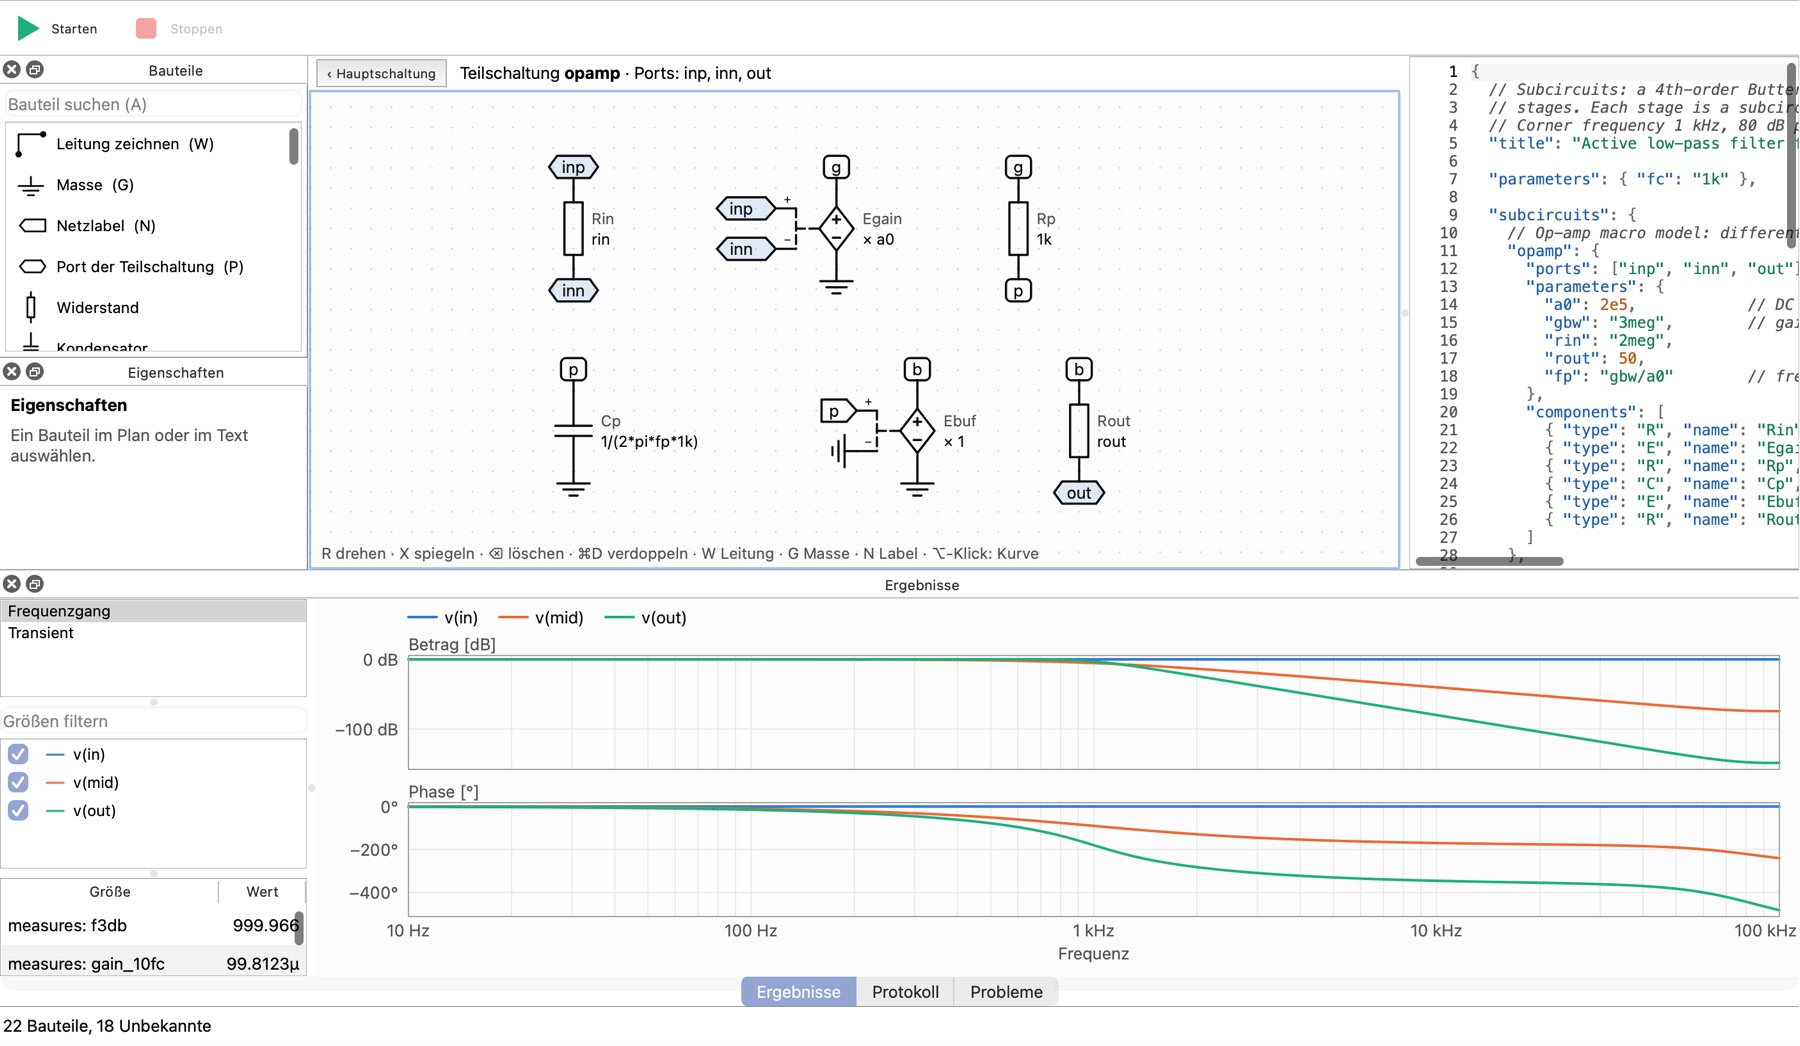
\includegraphics[width=\textwidth]{opamp_sub.jpg}
  \caption{Der Plan der Teilschaltung \code{opamp} aus
    \code{examples/opamp_filter.json}. Oben die Leiste mit dem Weg zurück
    und den Ports, im Plan die Ports \code{inp}, \code{inn} und \code{out}
    als beidseitig spitze Symbole.}
  \label{abb:opamp-sub}
\end{figure}

\section{Öffnen und zurück}

\begin{itemize}
  \item \textbf{Doppelklick} auf eine Instanz öffnet den Plan ihrer
    Teilschaltung (ebenso \menue{Teilschaltung „…“ öffnen} im
    Kontextmenü).
  \item Steht der Textcursor in einem Bauteil innerhalb einer
    Teilschaltung, wechselt der Plan von selbst dorthin.
  \item Über dem Plan steht dann eine Leiste: \menue{\guilsinglleft\ Hauptschaltung},
    der Name der Teilschaltung und ihre Ports.
  \item \menue{\guilsinglleft\ Hauptschaltung} oder \tasten{Strg}{$\uparrow$} führen zurück.
\end{itemize}

Im Plan einer Teilschaltung funktioniert alles wie in der Hauptschaltung;
dazu kommen die Ports.

\section{Ports}

Ein Port ist die Verbindung eines inneren Netzes nach außen. \taste{P} (oder
der Eintrag \menue{Port der Teilschaltung} in der Bauteilliste) fragt nach
dem Namen und setzt den Port per Klick. Ports verbinden wie Netzlabels über
ihren Namen.

\begin{itemize}
  \item Ein Port mit einem \emph{vorhandenen} Namen zeichnet einen Port der
    Teilschaltung an diese Stelle.
  \item Ein Port mit einem \emph{neuen} Namen erweitert die Ports: Der Name
    wird an \code{"ports"} angehängt, und jede Instanz bekommt einen
    Anschluss mehr (zunächst offen).
  \item Ports, die im Plan nicht gezeichnet sind, ergänzt der Editor am
    linken Rand.
\end{itemize}

\section{Eine neue, leere Teilschaltung}

\menue{Neue Teilschaltung \dots} in der Bauteilliste fragt nach dem Namen
und den Ports (durch Komma getrennt, z.\,B. \code{in, out, vdd}) und legt
unter \code{"subcircuits"} eine leere Definition an. Sie erscheint danach in
der Bauteilliste als »Teilschaltung „\textit{name}“« und wird wie jedes
andere Bauteil platziert. Ein Doppelklick auf die Instanz öffnet den noch
leeren Plan, in dem die Ports schon stehen.

\section{Auswahl in eine Teilschaltung umwandeln}
\label{sec:auslagern}

Aus einem Teil einer fertigen Schaltung wird so eine Teilschaltung:

\begin{enumerate}
  \item Die Bauteile im Plan auswählen (Rechteck aufziehen,
    Umschalt-Klick), samt ihrer Leitungen, Labels und Massen.
  \item \tasten{Strg}{G} drücken (oder \menue{In Teilschaltung umwandeln
    \dots} im Kontextmenü oder unter \menue{Bearbeiten}).
  \item Einen Namen für die Teilschaltung eingeben.
\end{enumerate}

Der Editor erledigt den Rest:

\begin{itemize}
  \item \textbf{Ports} werden die Netze, die Ausgewähltes mit dem Rest der
    Schaltung verbinden – von links nach rechts geordnet. Masse wird nie ein
    Port; sie ist überall dieselbe.
  \item Die \textbf{Grenze} liegt dort, wo ein nicht ausgewähltes Element
    ein ausgewähltes berührt. Innen sitzt dort der Port, außen ein Netzlabel
    mit dem Namen des Netzes, sodass alle Verbindungen erhalten bleiben.
  \item Die Bauteile wandern mit ihrem Text (Werte, Modelle, Kommentare)
    in die neue Definition, die Zeichnung mit ihnen.
  \item An ihrer Stelle steht eine Instanz mit Labels an den Anschlüssen.
\end{itemize}

Alles ist eine einzige Textänderung: \tasten{Strg}{Z} nimmt die ganze
Umwandlung in einem Schritt zurück. Die Schaltung rechnet vorher und
nachher dasselbe.

\section{Kurven und Spannungen in Teilschaltungen}

Im Plan einer Teilschaltung beziehen sich Kurven und Arbeitspunkt auf eine
Instanz. Ein \tasten{Alt}{Klick} auf das Netz \code{out} zeigt
\code{v(U1.out)}, wenn die Instanz \code{U1} heißt; ein Port steht für den
Knoten außen. Gibt es mehrere Instanzen, fragt der Editor, welche gemeint
ist. Die Spannungen an den Labels stehen nur, wenn die Teilschaltung genau
einmal verwendet wird.

Damit eine innere Größe als Kurve vorliegt, muss sie unter
\code{"outputs"} stehen (z.\,B. \code{"v(U1.mid)"}); die Statuszeile sagt,
was fehlt.

\section{SPICE-Teilschaltungen}

Teilschaltungen aus SPICE-Dateien (etwa Makromodelle von Operationsverstärkern
aus der Modellbibliothek) stehen als SPICE-Text in der Datei. Sie
erscheinen im Plan als Kasten mit den Ports der \code{.subckt}-Zeile, haben
aber keinen eigenen Plan: Ein Doppelklick zeigt ihren Text. Geändert werden
sie im Texteditor.

\chapter{Die Modellbibliothek}
\label{kap:editor-bibliothek}

Halbleiter brauchen Modellparameter, und fertige Bausteine wie
Operationsverstärker kommen als Teilschaltungen. Die Modellbibliothek
sammelt solche Modelle aus mehreren Quellen und kopiert ein gewähltes Modell
in die Datei. Die Datei bleibt dadurch vollständig: Sie rechnet auch auf
einem Rechner, der die Bibliothek nicht kennt.

\section{Quellen}

\begin{description}[style=nextline,leftmargin=2em]
  \item[Standardbibliothek]
    Ins Programm eingebaut (\datei{editor/library/standard.lib}). Sie
    enthält nur allgemeine Modelle mit Lehrbuchwerten, keine Bauteile
    bestimmter Hersteller:

    \begin{tabularx}{\linewidth}{@{}lL@{}}
      \toprule
      Name & Beschreibung \\
      \midrule
      \code{NPN_GEN}, \code{PNP_GEN} & Allgemeiner NPN- und PNP-Transistor \\
      \code{D_GEN} & Allgemeine Siliziumdiode, etwa 0,6\,V bei 1\,mA \\
      \code{Z5V1_GEN} & Z-Diode 5,1\,V, vereinfacht \\
      \code{NMOS_L1}, \code{PMOS_L1} & MOSFETs Level 1 mit Gate-Ladung \\
      \code{n18}, \code{p18} & MOSFETs BSIM3v3, typisch für 0,18\,µm \\
      \bottomrule
    \end{tabularx}
  \item[Beispiele]
    Die Modelle aus \code{"models"} der mitgelieferten Beispiele.
  \item[Eigene Bibliotheken]
    Dateien und ganze Ordner, die man selbst einbindet:
    \begin{itemize}
      \item SPICE-Dateien (\datei{.lib}, \datei{.mod}, \datei{.txt},
        \datei{.cir}, \datei{.sp}) mit \code{.model}-Karten und
        \code{.subckt}-Teilschaltungen, wie Hersteller sie veröffentlichen,
      \item esim-Dateien (\datei{.json}) mit ihrem Abschnitt
        \code{"models"}.
    \end{itemize}
\end{description}

\section{Eigene Bibliotheken einbinden}

Im Dialog \menue{Modellbibliothek} (\tasten{Strg}{L}) führt
\menue{Bibliotheken \dots} zur Liste der eigenen Bibliotheken.
\menue{Datei \dots} und \menue{Ordner \dots} fügen hinzu,
\menue{Entfernen} nimmt einen Eintrag wieder heraus. Ein Ordner wird mit
allen passenden Dateien gelesen. Die Liste bleibt über den Neustart
erhalten.

Beim Lesen einer SPICE-Datei gilt:
\begin{itemize}
  \item Fortsetzungszeilen (\code{+}) und Kommentare (\code{*}, \code{;})
    werden verstanden.
  \item Jede \code{.model}-Karte auf oberster Ebene ist ein Modell. Der
    Kommentar direkt über der Karte ist ihre Beschreibung; dessen erste
    Zeile erscheint in der Liste.
  \item Jeder \code{.subckt}-Block ist eine Teilschaltung. Er nimmt die
    \code{.model}- und \code{.subckt}-Definitionen der Datei mit, die er
    benutzt. Reine Hilfs-Teilschaltungen, die nur von anderen benutzt
    werden, erscheinen nicht in der Liste. Enthält eine Datei nur eine
    Teilschaltung, ist der Kommentarkopf der Datei ihre Beschreibung.
  \item Modelltypen, die esim nicht kennt, werden übergangen; was sich
    nicht lesen lässt, nennt der Dialog unter der Liste.
\end{itemize}

\begin{hinweis}[Modelle von Herstellern]
  Die Modelldateien der Halbleiterhersteller stehen meist auf deren
  Produktseiten (»SPICE model«, »PSpice model«). esim versteht die
  üblichen PSpice-Formen (Kapitel~\ref{kap:format-teilschaltungen}) und
  ist mit Makromodellen von Operationsverstärkern und mit
  Leistungs-MOSFETs (Level~3) erprobt. Weil die Lizenz solcher Dateien
  die Weitergabe oft nicht erlaubt, gehören sie in die eigene Bibliothek,
  nicht in ein öffentliches Projekt.
\end{hinweis}

\section{Der Dialog}

\menue{Bearbeiten}\pfad\menue{Modellbibliothek \dots} (\tasten{Strg}{L})
oder der Eintrag \menue{Modellbibliothek \dots} der Bauteilliste öffnet
den Dialog:

\begin{itemize}
  \item \textbf{Suchfeld}: sucht in Name, Beschreibung und Quelle.
  \item \textbf{Art}: Alle Arten, Dioden, Bipolartransistoren, MOSFETs,
    JFETs oder Teilschaltungen (SPICE).
  \item \textbf{Liste} mit Name, Art, Beschreibung und Quelle.
  \item \textbf{Karte}: der vollständige Text des gewählten Modells mit
    seiner Quelle.
\end{itemize}

Die Schaltflächen unten:
\begin{description}[leftmargin=2em]
  \item[Im Plan platzieren] kopiert das Modell in die Datei und hängt ein
    passendes Bauteil (Diode, Transistor, Instanz der Teilschaltung) mit
    diesem Modell an den Mauszeiger.
  \item[In die Datei übernehmen] kopiert nur das Modell nach
    \code{"models"} bzw. die Teilschaltung nach \code{"subcircuits"}.
  \item[Verwenden] (wenn der Dialog aus dem Feld \code{model} der
    Eigenschaften geöffnet wurde) setzt das Modell am gewählten Bauteil.
\end{description}

\section{Schneller: Suche in der Bauteilliste}

Für den Alltag ist der Dialog oft nicht nötig. Die Suche der Bauteilliste
findet auch die Modelle der Bibliothek: \taste{A}, »NPN\_GEN« tippen,
Eingabetaste – der Transistor hängt mit seinem Modell am Mauszeiger. Ebenso
schlägt das Feld \code{model} in den Eigenschaften beim Tippen passende
Modelle vor.

\section{Was in der Datei landet}

Ein Modell wird als SPICE-Zeile in \code{"models"} kopiert, lange Karten als
Liste ihrer Zeilen:

\begin{json}
"models": {
  "NPN_GEN": ".model NPN_GEN NPN(IS=1e-14 BF=200 BR=2 CJE=10p CJC=5p TF=0.5n)",
  "n18": [".model n18 NMOS (LEVEL=49 VERSION=3.1 TNOM=27 TOX=4.1E-9",
          "+ XJ=1E-7 NCH=2.3549E17 VTH0=0.3694303 ...)"]
}
\end{json}

Eine Teilschaltung landet als SPICE-Text unter \code{"subcircuits"},
zusammen mit allem, was sie braucht. Ist ein Modell gleichen Namens schon in
der Datei, wird es nicht noch einmal kopiert.

\chapter{Simulation und Ergebnisse}
\label{kap:editor-ergebnisse}

\section{Simulieren}

\tasten{Strg}{R} sichert die Datei und startet \esim. Während der Rechnung
zeigt die Statuszeile Analyse und Fortschritt in Prozent, das
\menue{Protokoll} die Ausgabe des Simulators. \tasten{Strg}{.} bricht ab.
Nach dem Ende erscheinen die Ergebnisse; die Auswahl von Analyse, Größen und
Zoom bleibt über neue Läufe hinweg erhalten, sodass man nach einer Änderung
direkt vergleichen kann.

Die Ergebnisdateien liegen in einem temporären Ordner des Editors. Wer die
CSV-Dateien weiterverwenden will, rechnet dieselbe Datei auf der
Kommandozeile (Kapitel~\ref{kap:kommandozeile}) oder aus Python.

\section{Das Ergebnisfeld}

\begin{figure}[htbp]
  \centering
  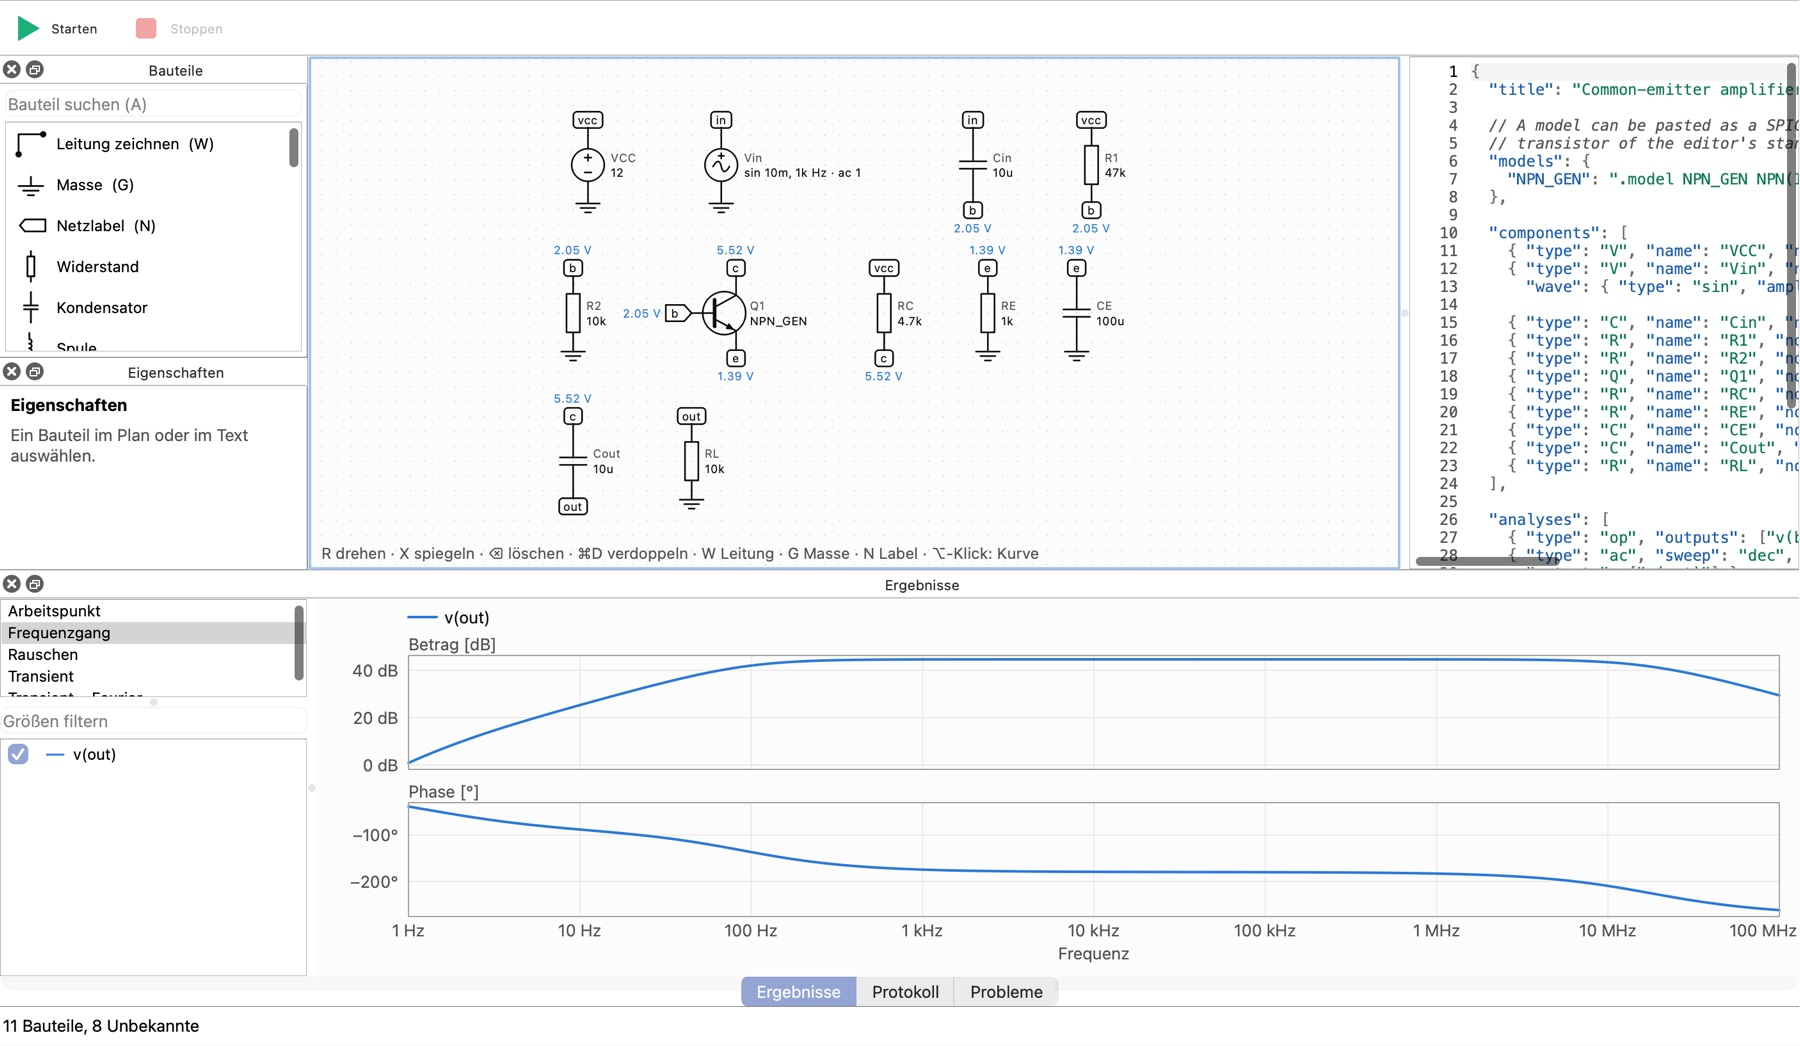
\includegraphics[width=\textwidth]{bjt_amplifier.jpg}
  \caption{Emitterschaltung (\code{examples/bjt_amplifier.json}) nach der
    Simulation: Spannungen des Arbeitspunkts an den Labels, unten der
    Frequenzgang als Betrag in dB und Phase.}
  \label{abb:bjt}
\end{figure}

Links oben steht die Liste der \textbf{Analysen} der Datei, mit deutschen
Namen (\menue{Arbeitspunkt}, \menue{DC-Sweep}, \menue{Frequenzgang},
\menue{Transient}, \menue{Periodischer Zustand}, \menue{Rauschen},
\menue{Empfindlichkeit}, \menue{Anpassung}). Benannte Analysen tragen
ihren Namen, Studien den Zusatz »(Sweep)« oder »(Monte Carlo)«. Haben
Analysen Messgrößen über viele Läufe oder eine Fourier-Analyse, kommen
Einträge »– Messgrößen« und »– Fourier« hinzu.

Darunter die \textbf{Größen} der gewählten Analyse mit Häkchen, ein Feld zum
Filtern (z.\,B. »v(« für alle Spannungen) und die \textbf{Wertetabelle}:
Arbeitspunkt, Messgrößen, Statistik der Rechnung (Schritte, Iterationen,
Ereignisse) und bei Monte Carlo Mittelwert, Streuung, Minimum und
Maximum. Eine Messung ohne Ergebnis steht als »nicht bestimmt« darin.

Rechts die \textbf{Kurven}.

\section{Kurven}

Die Kurven einer Analyse stehen in übereinanderliegenden Feldern mit
gemeinsamer $x$-Achse:

\begin{itemize}
  \item \textbf{Zeitverläufe} und \textbf{DC-Sweeps}: ein Feld für
    Spannungen, eines für Ströme, eines für alle übrigen Größen.
  \item \textbf{Frequenzgänge}: Betrag in dB und Phase in Grad über
    logarithmischer Frequenz.
  \item \textbf{Rauschen}: die Rauschdichten über der Frequenz.
  \item \textbf{Sweeps}: eine Kurve je Parameterwert in Stufen einer
    Blauskala; die Legende nennt die Werte.
\end{itemize}

\begin{center}
\begin{tabularx}{\textwidth}{@{}P{5.2cm}L@{}}
  \toprule
  Bedienung & Wirkung \\
  \midrule
  Mausrad, Touchpad auf/ab, spreizen & Zoomt in $x$ um den Mauszeiger. \\
  \taste{Strg} + Mausrad & Zoomt in $y$ im Feld unter dem Mauszeiger. \\
  Touchpad seitwärts & Verschiebt in $x$. \\
  Ziehen mit der Maus & Zoomt auf das aufgezogene Rechteck. \\
  Doppelklick, \tasten{Strg}{0} & Zeigt alles. \\
  Maus über den Kurven & Fadenkreuz mit den Werten aller Kurven an dieser Stelle. \\
  Rechtsklick & \menue{Alles zeigen}, \menue{Als Bild speichern \dots} (PNG). \\
  \bottomrule
\end{tabularx}
\end{center}

Beim Zoomen in $x$ passt sich die $y$-Achse jedes Felds dem sichtbaren
Ausschnitt an. Die Kurven werden je Bildpunkt auf Minimum und Maximum
verdichtet; auch Millionen von Punkten bleiben deshalb flüssig und ohne
verschluckte Spitzen.

\paragraph{Kurven aus dem Plan.}
\tasten{Alt}{Klick} auf eine Leitung zeigt deren Spannung, auf ein Bauteil
dessen Strom, ebenso \menue{Spannung v(…) zeigen} und \menue{Strom i(…)
zeigen} im Kontextmenü. Der Editor zeigt die Größe in einer Analyse, die
sie enthält, und hakt sie an. Gespeichert sind nur Größen, die unter \code{"outputs"}
stehen (oder alle, wenn die Datei kein \code{"outputs"} hat).

\section{Messgrößen über viele Läufe}

Analysen mit \code{monte_carlo} oder \code{param_sweep} liefern ihre
Messgrößen je Lauf. Der Eintrag »– Messgrößen« zeigt sie in eigenen
Darstellungen, gewählt über \menue{Darstellung} und je Analyse gemerkt.

\subsection*{Monte Carlo: Histogramm}

Jede Messgröße bekommt ein eigenes Feld mit eigener Achse
(Abbildung~\ref{abb:mc}). Die Klassenbreite folgt der Regel von
Freedman und Diaconis. Der Mittelwert ist als Linie, der Bereich $\pm\sigma$
als Fläche markiert; die Kopfzeile nennt Anzahl $n$, Mittelwert $\mu$,
Standardabweichung $\sigma$, die relative Streuung $\sigma/\mu$, Minimum und
Maximum. Fährt die Maus über eine Klasse, zeigt ein Tooltip deren Bereich
und wie viele Läufe (und wie viel Prozent) hineinfallen. Ein Rechtsklick
sichert das Histogramm als Bild.

\begin{figure}[htbp]
  \centering
  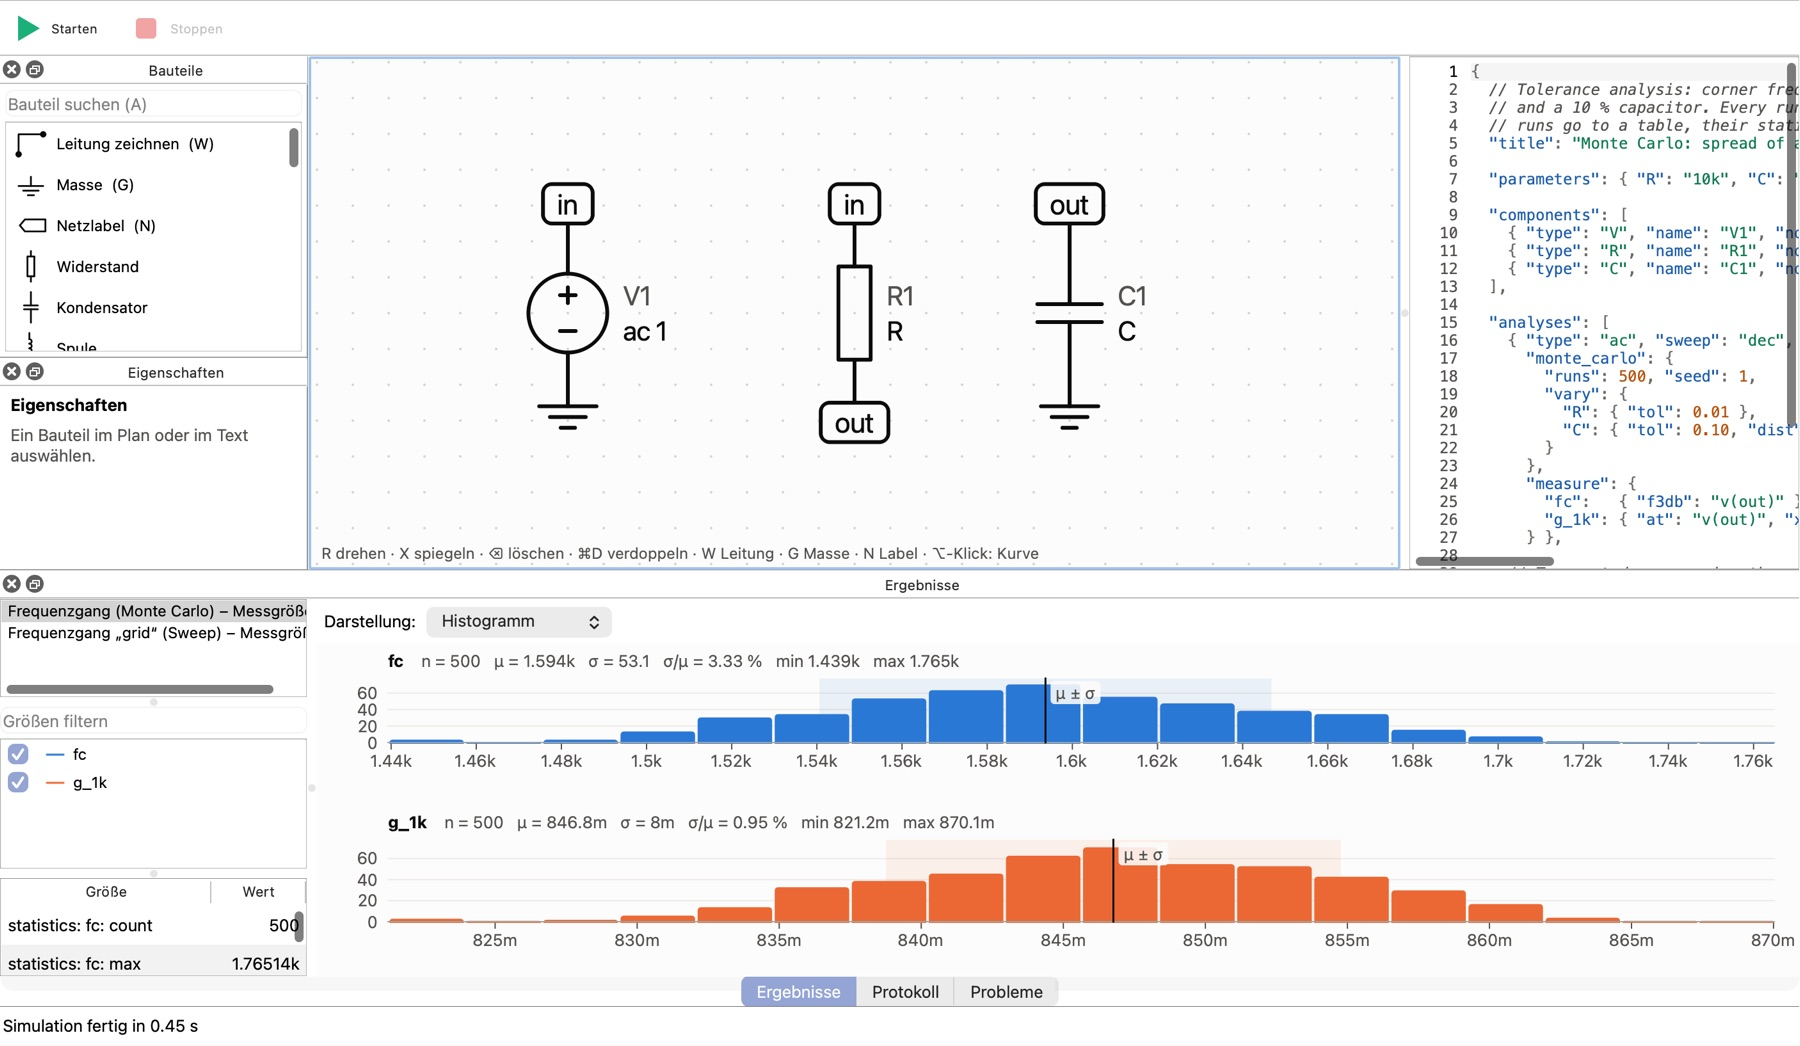
\includegraphics[width=\textwidth]{monte_carlo_filter.jpg}
  \caption{Monte-Carlo-Analyse eines RC-Filters
    (\code{examples/monte_carlo_filter.json}): 500 Läufe mit gestreutem $R$
    und $C$, Histogramme der Grenzfrequenz und der Verstärkung bei 1\,kHz.}
  \label{abb:mc}
\end{figure}

\subsection*{Monte Carlo: Streuung über einem Parameter}

\menue{Streuung über \textit{p}} zeigt jede Messgröße als Punktwolke über
dem gezogenen Wert des Parameters $p$. Daran sieht man, welcher Parameter
die Streuung verursacht: Eine schräge, schmale Wolke bedeutet starken
Einfluss, eine waagrechte keinen.

\subsection*{Sweeps: Kennlinie über dem Parameter}

Bei Parameter-Sweeps zeigt \menue{über \textit{p}} jede Messgröße als Linie
mit Punkten über dem Parameter, über mehrere Dekaden logarithmisch. Bei
verschachtelten Sweeps ergeben die weiteren Parameter eine Kurvenschar auf
der Blauskala – etwa die Periode eines Oszillators über $C$ für mehrere
Werte von $R$.

\section{Ein Beispiel mit Ereignissen}

\begin{figure}[htbp]
  \centering
  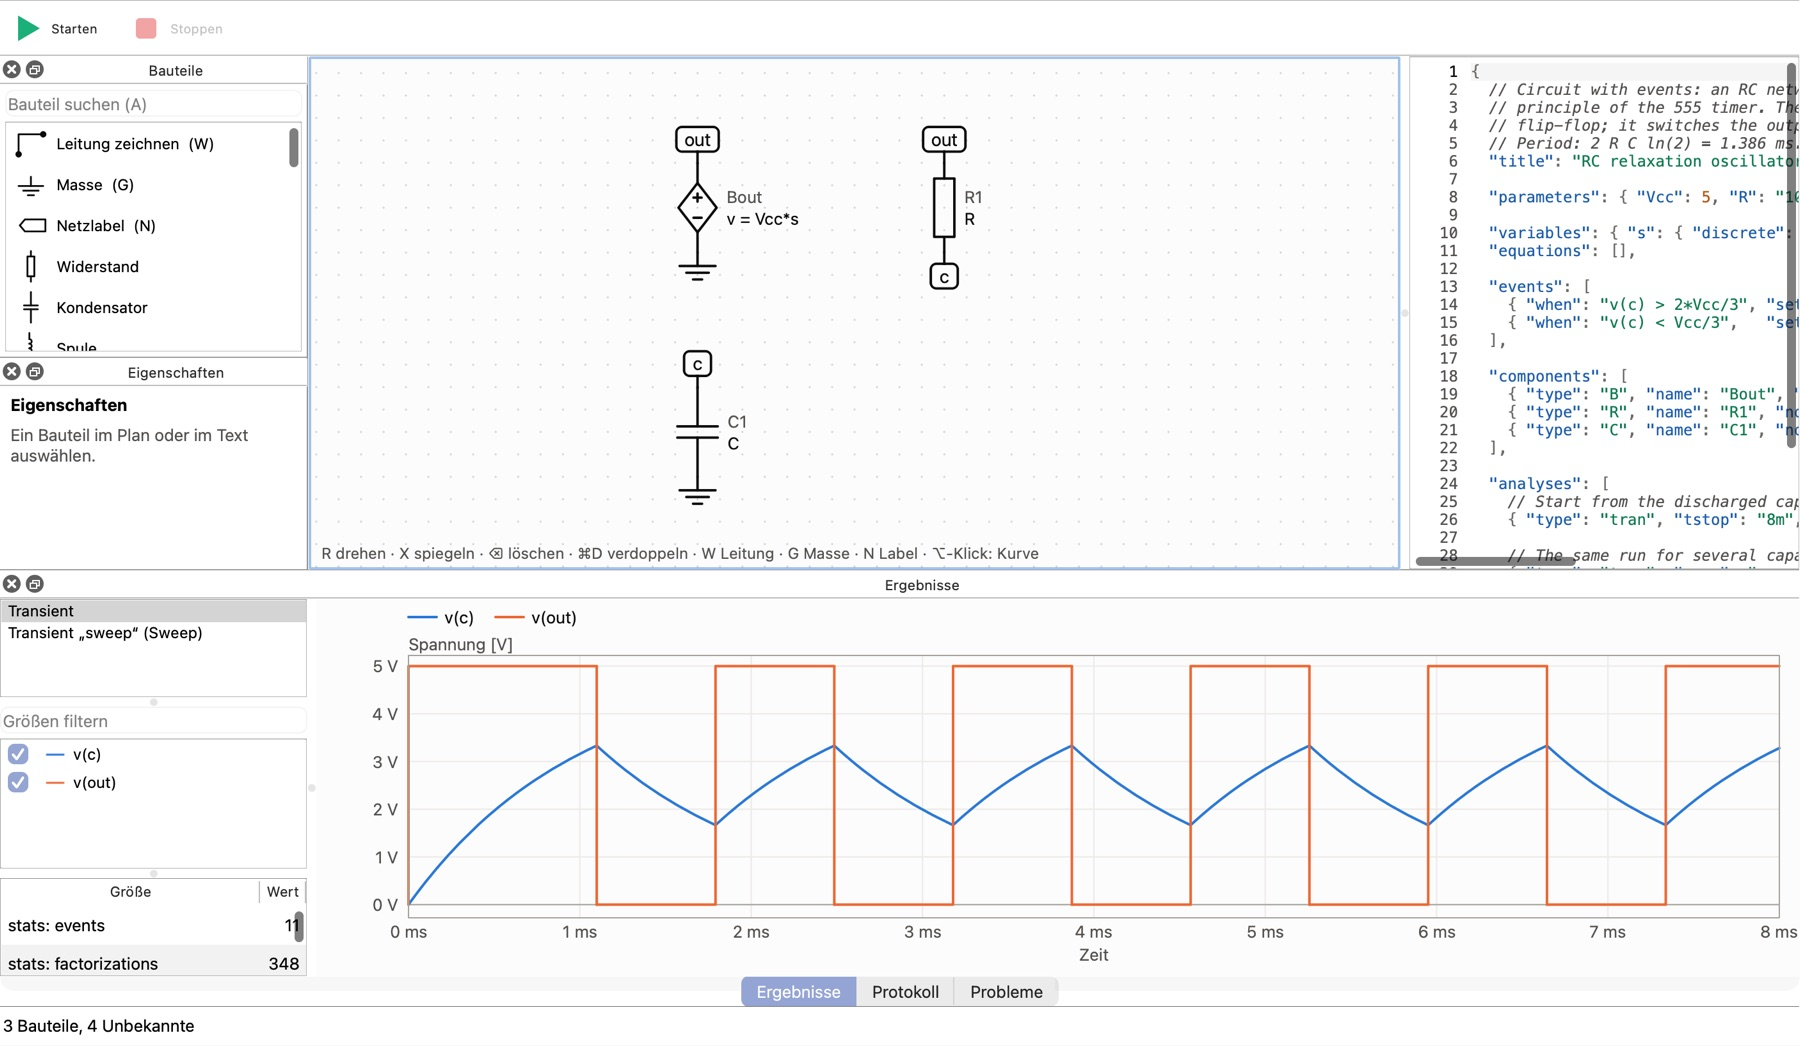
\includegraphics[width=\textwidth]{relaxation_oscillator.jpg}
  \caption{Kippschwinger nach dem Prinzip des 555
    (\code{examples/relaxation_oscillator.json}): Eine Verhaltensquelle
    schaltet über eine diskrete Variable \code{s}, die zwei Ereignisse
    setzen. Die Umschaltzeitpunkte sind exakt bestimmt.}
  \label{abb:relax}
\end{figure}

Abbildung~\ref{abb:relax} zeigt eine Schaltung ohne Schaltplan-Leitungen:
Die Datei hat keinen gezeichneten Plan, der Editor hat jedes Bauteil mit
Labels an den Anschlüssen angeordnet. Das Beispiel enthält außerdem einen
Sweep über $C$, dessen Kurvenschar unter »Transient „sweep“ (Sweep)«
erscheint.


\part{Die Eingabedatei}
\chapter{Aufbau der Eingabedatei}
\label{kap:format-grundlagen}

Dieser Teil beschreibt das Eingabeformat vollständig. Er gilt gleichermaßen
für Dateien, die im Editor entstehen, und für Dateien, die man von Hand
schreibt oder aus einem Programm erzeugt.

\section{Die Datei als Ganzes}

Eine Eingabedatei ist ein JSON-Objekt. Anders als reines JSON darf sie
Kommentare enthalten: \code{//} bis zum Zeilenende und \code{/* ... */}
über mehrere Zeilen. Die Kodierung ist UTF-8. Ein Komma nach dem letzten
Element einer Liste oder eines Objekts ist, wie in JSON, ein Fehler.

\begin{center}
\begin{tabularx}{\textwidth}{@{}lLl@{}}
  \toprule
  Schlüssel & Inhalt & Abschnitt \\
  \midrule
  \code{title} & Titel, erscheint auf der Konsole und im Ergebnis & \\
  \code{parameters} & benannte Konstanten & \ref{sec:parameter} \\
  \code{functions} & eigene Funktionen für Ausdrücke & \ref{sec:funktionen} \\
  \code{tables} & Kennlinien aus Stützstellen & \ref{sec:tabellen} \\
  \code{models} & Modellparameter von Halbleitern & \ref{kap:format-modelle} \\
  \code{subcircuits} & Teilschaltungen & \ref{kap:format-teilschaltungen} \\
  \code{components} & die Bauteile der Schaltung & \ref{kap:format-bauteile} \\
  \code{variables} & Unbekannte eigener Gleichungen & \ref{kap:format-gleichungen} \\
  \code{equations} & eigene Gleichungen & \ref{kap:format-gleichungen} \\
  \code{events} & Ereignisse mit Zuweisungen & \ref{sec:ereignisse} \\
  \code{analyses} & die Analysen, in dieser Reihenfolge gerechnet & \ref{kap:format-analysen} \\
  \code{outputs} & auszugebende Größen & \ref{sec:ausgaenge} \\
  \code{options} & Toleranzen, Temperatur, Verfahren & \ref{sec:optionen} \\
  \code{nodeset} & Startwerte für den Arbeitspunkt & \ref{sec:optionen} \\
  \code{ic} & Anfangsspannungen für \code{"uic"} & \ref{sec:optionen} \\
  \code{schematic} & der Schaltplan des Editors (vom Simulator überlesen) & \ref{kap:editor-schaltplan} \\
  \bottomrule
\end{tabularx}
\end{center}

Eine Datei enthält \code{components}, \code{equations} oder beides.
Unbekannte Schlüssel – auf oberster Ebene, an Bauteilen, Modellen oder
Analysen – erzeugen eine Warnung und werden übergangen. So fallen
Tippfehler auf, ohne dass die Rechnung abbricht. Die Schlüssel von Bauteilen
und Modellen unterscheiden nicht zwischen Groß- und Kleinschreibung
(\code{"Value"} ist \code{"value"}).

\section{Zahlen}
\label{sec:zahlen}

Ein Zahlenwert kann sein:

\begin{itemize}
  \item eine JSON-Zahl: \code{1000}, \code{4.7e3}, \code{-0.5},
  \item eine Zeichenkette mit SI-Präfix und optionaler Einheit:
    \code{"4.7k"}, \code{"100nF"}, \code{"2.2M"}, \code{"10meg"},
  \item ein Ausdruck aus Zahlen und Parametern: \code{"2*R0"},
    \code{"1/(2*pi*R0*C0)"}.
\end{itemize}

\begin{center}
\begin{tabular}{@{}*{9}{c}@{}}
  \toprule
  \code{f} & \code{p} & \code{n} & \code{u}, \texttt{µ} & \code{m} &
  \code{k}, \code{K} & \code{M}, \code{meg} & \code{G} & \code{T} \\
  \midrule
  $10^{-15}$ & $10^{-12}$ & $10^{-9}$ & $10^{-6}$ & $10^{-3}$ &
  $10^{3}$ & $10^{6}$ & $10^{9}$ & $10^{12}$ \\
  \bottomrule
\end{tabular}
\end{center}

\begin{achtung}[Groß- und Kleinschreibung]
  Anders als in SPICE unterscheiden die Präfixe Groß- und Kleinschreibung:
  \code{"1M"} ist ein Megaohm, \code{"1m"} ein Milliohm. \code{meg} ist
  immer Mega. In SPICE-Text (Modellkarten, SPICE-Teilschaltungen) gilt
  dagegen die SPICE-Regel: \code{M} ist dort Milli.
\end{achtung}

Buchstaben nach dem Präfix gelten als Einheit und werden ignoriert:
\code{"100nF"} ist $10^{-7}$, \code{"1F"} ist 1 (ein Farad, nicht ein Femto).
In Ausdrücken ist nur das Präfix erlaubt (\code{"4.7k*2"}), keine Einheit.
Zahlen werden unabhängig von den Ländereinstellungen des Rechners gelesen;
das Dezimalzeichen ist immer der Punkt.

\section{Parameter}
\label{sec:parameter}

Parameter sind benannte Konstanten. Sie dürfen sich aufeinander beziehen,
die Reihenfolge spielt keine Rolle:

\begin{json}
"parameters": { "R0": "1k", "C0": "100n", "tau": "R0*C0", "fc": "1/(2*pi*tau)" }
\end{json}

Parameter können überall verwendet werden, wo eine Zahl steht – in
Bauteilwerten, Modellparametern, Analysen (\code{"tstop": "10*tau"}), in
Gleichungen und Ausgängen. Parameter-Sweeps, Monte Carlo,
Empfindlichkeiten und die Anpassung an Messdaten verändern Parameter; alles,
was von ihnen abhängt, wird für jeden Lauf neu berechnet. Wer eine Größe
später variieren will, schreibt sie deshalb am besten gleich als Parameter.

\section{Ausdrücke}
\label{sec:ausdruecke}

Ausdrücke stehen in Gleichungen, Verhaltensquellen, Ausgängen, Ereignissen,
Schaltern und überall, wo eine Zahl erwartet wird (dort nur mit
Parametern).

\begin{center}
\begin{tabularx}{\textwidth}{@{}P{3.3cm}L@{}}
  \toprule
  Element & Schreibweise \\
  \midrule
  Grundrechenarten & \code{+ - * /}, Potenz \code{^} oder \code{**}, Klammern \\
  Vergleiche & \code{< <= > >= == !=} (Ergebnis 1 oder 0) \\
  Logik & \code{&&}, \code{||}, \code{!} \\
  Fallunterscheidung & \code{if(bedingung, dann, sonst)} \\
  Funktionen & \code{sin cos tan asin acos atan atan2(y,x) sinh cosh tanh exp log ln log10 sqrt abs sign min(a,b) max(a,b) pow(a,b)} \\
  Konstanten & \code{pi} \\
  Zeit & \code{t} oder \code{time} \\
  Schaltungsgrößen & \code{v(knoten)}, \code{v(a,b)} $=$ \code{v(a)-v(b)}, \code{i(bauteil)} \\
  Variablen & Namen aus \code{variables}, Elemente \code{T[i]} von Vektoren \\
  Tabellen & \code{name(x)} für eine Kennlinie aus \code{tables} \\
  eigene Funktionen & \code{name(a, b)} aus \code{functions} \\
  Totzeit & \code{delay(x, td)} (Abschnitt~\ref{sec:totzeit}) \\
  Summe & \code{sum(i, von, bis, ausdruck)} (Abschnitt~\ref{sec:vektoren}) \\
  Zeitableitung & \code{der(ausdruck)}, nur in Gleichungen \\
  \bottomrule
\end{tabularx}
\end{center}

\code{log} und \code{ln} sind beide der natürliche Logarithmus; den
dekadischen liefert \code{log10}. Winkel sind im Bogenmaß.

Die Ableitungen für das Newton-Verfahren werden automatisch und exakt
gebildet. Unstetige Ausdrücke – Vergleiche, \code{if}, \code{abs},
\code{sign}, \code{min}, \code{max} – sind in Gleichungen und
Verhaltensquellen erlaubt: Die Stelle, an der ein Vergleich kippt, wird als
Ereignis exakt bestimmt (Abschnitt~\ref{sec:ereignisse}).

\section{Eigene Funktionen}
\label{sec:funktionen}

Wiederkehrende Ausdrücke lassen sich als Funktionen ablegen:

\begin{json}
"functions": {
  "clip(x, lim)":   "max(-lim, min(lim, x))",
  "core(i, L, is)": "L*is*tanh(i/is)"
}
\end{json}

Ein Aufruf wird durch den Rumpf ersetzt, mit den Argumenten anstelle der
Parameter. Funktionen dürfen Parameter der Datei und andere Funktionen
verwenden, sich aber nicht selbst aufrufen und keine eingebaute Funktion
überschreiben. Sie stehen in Gleichungen, Verhaltensquellen, Schaltern,
Ereignissen und Ausgängen zur Verfügung, nicht aber in reinen Zahlenwerten
(Bauteilwerte, \code{parameters}).

\section{Tabellen}
\label{sec:tabellen}

Kennlinien aus Stützstellen, etwa Messdaten oder Datenblattkurven, werden
unter \code{tables} definiert und in Ausdrücken wie eine Funktion mit einem
Argument aufgerufen:

\begin{json}
"tables": {
  "cell": { "x": [0, 0.3, 0.5, 0.6], "y": [3.0, 2.96, 2.38, 0], "interp": "cubic" },
  "ntc":  { "file": "ntc_curve.csv", "xcol": 0, "ycol": 1 }
},
"components": [
  { "type": "B", "name": "Bcell", "nodes": ["0", "p"], "i": "cell(v(p))" }
]
\end{json}

\begin{description}[style=nextline,leftmargin=2em]
  \item[Daten]
    \code{x} und \code{y} als Listen, oder \code{points} als Liste von
    Paaren \code{[x, y]}, oder \code{file}: eine Textdatei mit
    Zahlenspalten. Trenner sind Komma, Semikolon oder Leerzeichen; Zeilen,
    die nicht mit einer Zahl beginnen (Überschriften), werden übersprungen.
    Der Pfad gilt relativ zur Eingabedatei; \code{xcol} und \code{ycol}
    wählen die Spalten (gezählt ab 0). \code{x} muss streng steigen.
  \item[{\code{interp}}]
    \code{"linear"} (Standard) oder \code{"cubic"}. Die kubische
    Interpolation ist monoton (PCHIP): glatte Steigung, aber kein
    Überschwingen zwischen den Stützstellen. Für Kennlinien in Gleichungen
    und Quellen ist sie meist die bessere Wahl, weil das Newton-Verfahren
    dann eine stetige Ableitung sieht.
  \item[{\code{extrap}}]
    Außerhalb der Daten wird der Randwert gehalten (\code{"hold"},
    Standard) oder mit der Randsteigung fortgesetzt (\code{"linear"}).
\end{description}

\subsection*{Kennfelder über zwei Größen}

Ein Kennfeld, etwa die Flussverkettung über Strom und Position aus einer
Feldrechnung, wird mit \code{z} oder \code{zcol} angelegt und mit zwei
Argumenten aufgerufen, \code{name(x, y)}:

\begin{json}
"tables": {
  "psi": { "x": [0, 1, 2], "y": [0, 5e-3, 1e-2],
           "z": [[0, 0, 0], [0.01, 0.006, 0.004], [0.018, 0.011, 0.007]],
           "interp": "cubic" },
  "map": { "file": "kennfeld.csv", "xcol": 0, "ycol": 1, "zcol": 2 }
},
"components": [
  { "type": "B", "name": "L1", "nodes": ["a", "0"], "phi": "psi(i(L1), z)" }
]
\end{json}

\code{z[i][j]} gehört zu \code{(x[i], y[j])}. Eine Datei enthält einen Punkt
je Zeile in beliebiger Reihenfolge und muss das ganze Gitter abdecken.
\code{x} und \code{y} müssen streng steigen. \code{"linear"} ist bilinear;
\code{"cubic"} ist ein Tensorprodukt kubischer Hermite-Interpolanten mit
stetiger Steigung und exakten Ableitungen für das Newton-Verfahren, aber
(anders als bei der Kennlinie) nicht monoton. \code{extrap} gilt für beide
Achsen.

\section{Knoten}

Knotennamen sind beliebige Zeichenketten oder ganze Zahlen. Masse heißt
\code{"0"} oder \code{"gnd"}. Jede Schaltung braucht einen Massebezug, und
jeder Knoten braucht einen Gleichstrompfad nach Masse
(Abschnitt~\ref{sec:schwebend}). In Ausdrücken (\code{v(...)}) sind nur
Knotennamen ohne Komma und Klammern verwendbar; einfache Namen wie
\code{out}, \code{vdd}, \code{n12} sind deshalb am praktischsten.

Größen innerhalb von Teilschaltungen heißen von außen
\code{<Instanz>.<Name>}, etwa \code{v(X1.mid)} oder \code{i(U1.V1)}
(Kapitel~\ref{kap:format-teilschaltungen}).

\chapter{Bauteile}
\label{kap:format-bauteile}

\section{Allgemeines}

Jedes Bauteil ist ein Objekt in der Liste \code{components}:

\begin{json}
{ "type": "R", "name": "R1", "nodes": ["in", "out"], "value": "4.7k" }
\end{json}

\begin{description}[style=nextline,leftmargin=2em]
  \item[\code{type}] der SPICE-Buchstabe oder der lange Name (\code{"R"} oder
    \code{"resistor"}); Groß- und Kleinschreibung egal.
  \item[\code{name}] optional, aber nötig für \code{i(...)}, als Quelle eines
    DC-Sweeps, als Steuerung gesteuerter Quellen und für die Kopplung.
    Bauteile ohne Namen bekommen einen aus Typ und Position (\code{V2}).
  \item[\code{nodes}] die Knoten in der Reihenfolge der Tabelle unten.
  \item[weitere Schlüssel] die Werte und Parameter des Bauteils.
\end{description}

\section{Übersicht}

\begin{longtable}{@{}P{2.6cm}P{3.6cm}P{2.6cm}P{5.0cm}@{}}
  \toprule
  \code{type} & Bauteil & \code{nodes} & Parameter \\
  \midrule
  \endhead
  \bottomrule
  \endfoot
  \code{R}, \code{resistor} & Widerstand & a, b & \code{value}; \code{"noise": false} ohne thermisches Rauschen \\
  \code{C}, \code{capacitor} & Kondensator & a, b & \code{value}, \code{ic} (Spannung a$-$b bei $t=0$) \\
  \code{L}, \code{inductor} & Spule & a, b & \code{value}, \code{ic} (Strom a$\to$b bei $t=0$) \\
  \code{V}, \code{vsource} & Spannungsquelle & $+$, $-$ & \code{dc}, \code{wave}, \code{ac}, \code{acphase} \\
  \code{I}, \code{isource} & Stromquelle & von, nach & \code{dc}, \code{wave}, \code{ac}, \code{acphase} \\
  \code{E}, \code{vcvs} & spannungsgesteuerte Spannungsquelle & $+$, $-$, Steuer$+$, Steuer$-$ & \code{gain} \\
  \code{G}, \code{vccs} & spannungsgesteuerte Stromquelle & von, nach, Steuer$+$, Steuer$-$ & \code{gm} \\
  \code{F}, \code{cccs} & stromgesteuerte Stromquelle & von, nach & \code{control}, \code{gain} \\
  \code{H}, \code{ccvs} & stromgesteuerte Spannungsquelle & $+$, $-$ & \code{control}, \code{r} \\
  \code{B}, \code{behavioral} & Verhaltensquelle & $+$, $-$ & genau eines von \code{i}, \code{v}, \code{q}, \code{phi} \\
  \code{K}, \code{coupling} & magnetische Kopplung & – & \code{inductors}, \code{k} \\
  \code{T}, \code{tline} & Leitung & Tor 1 ($+$, $-$), Tor 2 ($+$, $-$) & \code{z0}, \code{td} oder \code{f}/\code{nl} oder \code{l}/\code{c}/\code{len}; Verluste \code{r}, \code{g}, \code{segments} \\
  \code{S}, \code{switch} & idealer Schalter & a, b [, Steuer$+$, Steuer$-$] & \code{control}, \code{vt}, \code{vh}, \code{ron}, \code{roff}, \code{initial} \\
  \code{ideal_diode} & ideale Diode & Anode, Kathode & \code{vf}, \code{ron}, \code{roff} \\
  \code{D}, \code{diode} & Diode & Anode, Kathode & \code{model} oder Parameter (Kapitel~\ref{kap:format-modelle}) \\
  \code{Q}, \code{npn}, \code{pnp} & Bipolartransistor & C, B, E & \code{model} oder Parameter \\
  \code{J}, \code{njf}, \code{pjf} & Sperrschicht-FET & D, G, S & \code{model} oder Parameter \\
  \code{M}, \code{nmos}, \code{pmos} & MOSFET & D, G, S [, Bulk] & \code{model}, \code{w}, \code{l}, Parameter \\
  \code{X}, \code{subcircuit} & Instanz einer Teilschaltung & in der Reihenfolge der \code{ports} & \code{subcircuit}, \code{parameters} \\
\end{longtable}

\section{Widerstand, Kondensator, Spule}

\begin{json}
{ "type": "R", "name": "R1", "nodes": ["a", "b"], "value": "10k" },
{ "type": "C", "name": "C1", "nodes": ["b", "0"], "value": "100n", "ic": 2.5 },
{ "type": "L", "name": "L1", "nodes": ["b", "c"], "value": "1m",   "ic": "10m" }
\end{json}

\code{value} darf ein Ausdruck aus Parametern sein. \code{ic} ist der
Anfangswert für eine Transientenanalyse mit \code{"uic": true}
(Abschnitt~\ref{sec:tran}). Widerstände rauschen thermisch; mit
\code{"noise": false} nicht (nützlich für Hilfswiderstände in
Makromodellen). Nichtlineare Widerstände, Kondensatoren und Spulen
entstehen mit der Verhaltensquelle \code{B}.

\section{Unabhängige Quellen}
\label{sec:quellen}

\begin{json}
{ "type": "V", "name": "Vcc", "nodes": ["vcc", "0"], "dc": 12 },
{ "type": "V", "name": "Vin", "nodes": ["in", "0"], "dc": 0, "ac": 1,
  "wave": { "type": "sin", "amplitude": "10m", "freq": "1k" } },
{ "type": "I", "name": "Ib", "nodes": ["0", "b"], "dc": "10u" }
\end{json}

\begin{itemize}
  \item \code{dc} ist der Wert für Arbeitspunkt, DC-Sweep und den
    Arbeitspunkt der AC-Analyse. Ohne \code{dc} gilt dort der Wert von
    \code{wave} bei $t=0$.
  \item \code{wave} beschreibt den Zeitverlauf für die Transientenanalyse.
  \item \code{ac} (Amplitude, Standard 0) und \code{acphase} (Grad) sind die
    Kleinsignalanregung der AC-Analyse.
\end{itemize}

\begin{center}
\begin{tabularx}{\textwidth}{@{}lL@{}}
  \toprule
  \code{wave.type} & Parameter \\
  \midrule
  \code{sin} & \code{offset}, \code{amplitude}, \code{freq}, \code{delay}, \code{damping} (1/s), \code{phase} (Grad) \\
  \code{pulse} & \code{v1}, \code{v2}, \code{delay}, \code{rise}, \code{fall}, \code{width}, \code{period} \\
  \code{pwl} & \code{points}: \code{[[t0, v0], [t1, v1], ...]} \\
  \code{dc} & \code{value} \\
  \bottomrule
\end{tabularx}
\end{center}

\paragraph{Sinus.}
$v(t) = \mathit{offset} + \mathit{amplitude}\cdot
e^{-\mathit{damping}\,(t-\mathit{delay})}
\sin\bigl(2\pi\,\mathit{freq}\,(t-\mathit{delay}) + \mathit{phase}\bigr)$
für $t \geq \mathit{delay}$, davor der Wert bei $t = \mathit{delay}$. Sinusquellen
begrenzen die Schrittweite auf ein Zwanzigstel ihrer Periode.

\paragraph{Puls.}
Von \code{v1} nach \code{delay} in der Zeit \code{rise} auf \code{v2}, dort
\code{width} lang, in \code{fall} zurück. Mit \code{period} wiederholt sich
das, ohne \code{period} ist es ein Einzelpuls. \code{rise} und
\code{fall} sind ohne Angabe 0,1\,\% der Periode. Die Ecken des Pulses
werden als Haltepunkte exakt getroffen.

\paragraph{Stückweise linear.}
\code{points} sind Paare aus Zeit und Wert; zwischen ihnen wird linear
interpoliert, nach dem letzten der letzte Wert gehalten. Jede Stützstelle
ist ein Haltepunkt.

\paragraph{Vorzeichen.}
\code{i(V1)} ist der Strom vom Plus-Knoten \emph{durch die Quelle} zum
Minus-Knoten – also negativ, solange die Quelle Leistung abgibt (wie in
SPICE). Eine Stromquelle treibt ihren Strom vom ersten Knoten durch die
Quelle zum zweiten; \code{["0", "b"]} speist also in den Knoten \code{b}.

\section{Gesteuerte Quellen}

\begin{json}
{ "type": "E", "name": "E1", "nodes": ["out", "0", "inp", "inn"], "gain": 1e5 },
{ "type": "G", "name": "G1", "nodes": ["0", "x", "a", "b"], "gm": "1m" },
{ "type": "F", "name": "F1", "nodes": ["0", "y"], "control": "Vsense", "gain": 100 },
{ "type": "H", "name": "H1", "nodes": ["z", "0"], "control": "L1", "r": "1k" }
\end{json}

\code{E} und \code{G} werden von der Spannung zwischen den Steuerknoten
gesteuert, \code{F} und \code{H} vom Strom eines Bauteils mit Zweigstrom:
einer Spannungsquelle oder einer Spule (\code{control}). Um einen beliebigen
Strom zu messen, schaltet man eine Spannungsquelle mit 0\,V in Reihe.
Nichtlineare oder mehrfach gesteuerte Quellen sind Verhaltensquellen.

\section{Verhaltensquelle B}
\label{sec:bquelle}

Die Verhaltensquelle ist das vielseitigste Bauteil: Strom, Spannung, Ladung
oder Fluss sind ein beliebiger Ausdruck aus Knotenspannungen, Strömen,
Variablen, Parametern, Tabellen und der Zeit.

\begin{description}[style=nextline,leftmargin=2em]
  \item[{\code{"i": "..."}}]
    Strom vom Plus-Knoten durch das Bauteil zum Minus-Knoten. Ein
    nichtlinearer Widerstand: \code{"i": "1e-3*tanh(v(a,b)/0.1)"}.
  \item[{\code{"v": "..."}}]
    Spannung zwischen den Knoten; das Bauteil hat einen eigenen Zweigstrom
    \code{i(Name)}.
  \item[{\code{"q": "..."}}]
    Gespeicherte Ladung; der Strom ist ihre Zeitableitung. Ein
    spannungsabhängiger Kondensator: \code{"q": "C0*v(a,b) + C1*v(a,b)^2"}.
  \item[{\code{"phi": "..."}}]
    Magnetischer Fluss; die Spannung ist seine Zeitableitung. Der Ausdruck
    hängt in der Regel vom eigenen Strom ab. Eine sättigende Drossel:
    \code{"phi": "L0*Isat*tanh(i(L1)/Isat)"}.
\end{description}

Die Ableitungen nach allen vorkommenden Größen bildet esim selbst; auch in
der AC- und Rauschanalyse ist die Verhaltensquelle deshalb richtig
linearisiert. Vergleiche und \code{if} in Verhaltensquellen schalten als
Ereignis (Abschnitt~\ref{sec:ereignisse}). Verhaltensquellen rauschen
nicht.

\section{Magnetische Kopplung K}

\begin{json}
{ "type": "L", "name": "L1", "nodes": ["p1", "p2"], "value": "10m" },
{ "type": "L", "name": "L2", "nodes": ["s1", "s2"], "value": "1m" },
{ "type": "K", "name": "K1", "inductors": ["L1", "L2"], "k": 0.99 }
\end{json}

Die Kopplung verbindet zwei Spulen mit der Gegeninduktivität
$M = k\sqrt{L_1 L_2}$, $-1 < k < 1$. Der erste Knoten jeder Spule trägt den
Wicklungspunkt. Ein Übertrager mit dem Übersetzungsverhältnis $n$ hat
$L_2 = n^2 L_1$.

\section{Schalter S}
\label{sec:schalter}

\begin{json}
{ "type": "S", "name": "S1", "nodes": ["in", "sw", "gate", "0"], "vt": 0.5 },
{ "type": "S", "name": "S2", "nodes": ["a", "b"], "control": "i(L1)", "vt": "1", "vh": "0.1" }
\end{json}

\begin{itemize}
  \item Mit vier Knoten steuert die Spannung zwischen den Steuerknoten (wie
    in SPICE), mit zwei Knoten ein beliebiger Ausdruck in \code{control}:
    \code{"v(gate)"}, \code{"i(L1)"}, \code{"sin(2*pi*50*t)"}, eine
    Variable \dots
  \item Der Schalter schließt, wenn die Steuergröße über $v_t + v_h$
    steigt, und öffnet, wenn sie unter $v_t - v_h$ fällt (\code{vt}
    Schwelle, \code{vh} halbe Breite der Hysterese, beide Standard 0).
  \item \code{ron} (Standard 1\,m\ohm) und \code{roff} (Standard
    1\,G\ohm) sind die Widerstände in beiden Stellungen.
  \item \code{"initial": "on"} legt die Stellung fest, solange die
    Steuergröße beim Start innerhalb der Hysterese liegt.
\end{itemize}

\section{Ideale Diode}

\begin{json}
{ "type": "ideal_diode", "name": "D1", "nodes": ["0", "sw"], "vf": 0.4 }
\end{json}

Sie sperrt unterhalb der Flussspannung \code{vf} (Standard 0) mit
\code{roff} und leitet darüber mit der Steigung $1/r_\text{on}$. Im
Unterschied zur Diode \code{D} hat sie keine Exponentialkennlinie und keine
Ladung; sie ist für Leistungselektronik und Gleichrichter gedacht, wenn nur
das Schaltverhalten interessiert.

Schalter und ideale Dioden schalten als Ereignis: Der Umschaltzeitpunkt
wird exakt bestimmt. Hängen mehrere voneinander ab – ein Schalter öffnet an
einer Spule, also muss die Freilaufdiode leiten –, stellen sie sich im
selben Zeitpunkt gemeinsam ein, ohne künstliche Spannungsspitze.

\begin{figure}[htbp]
  \centering
  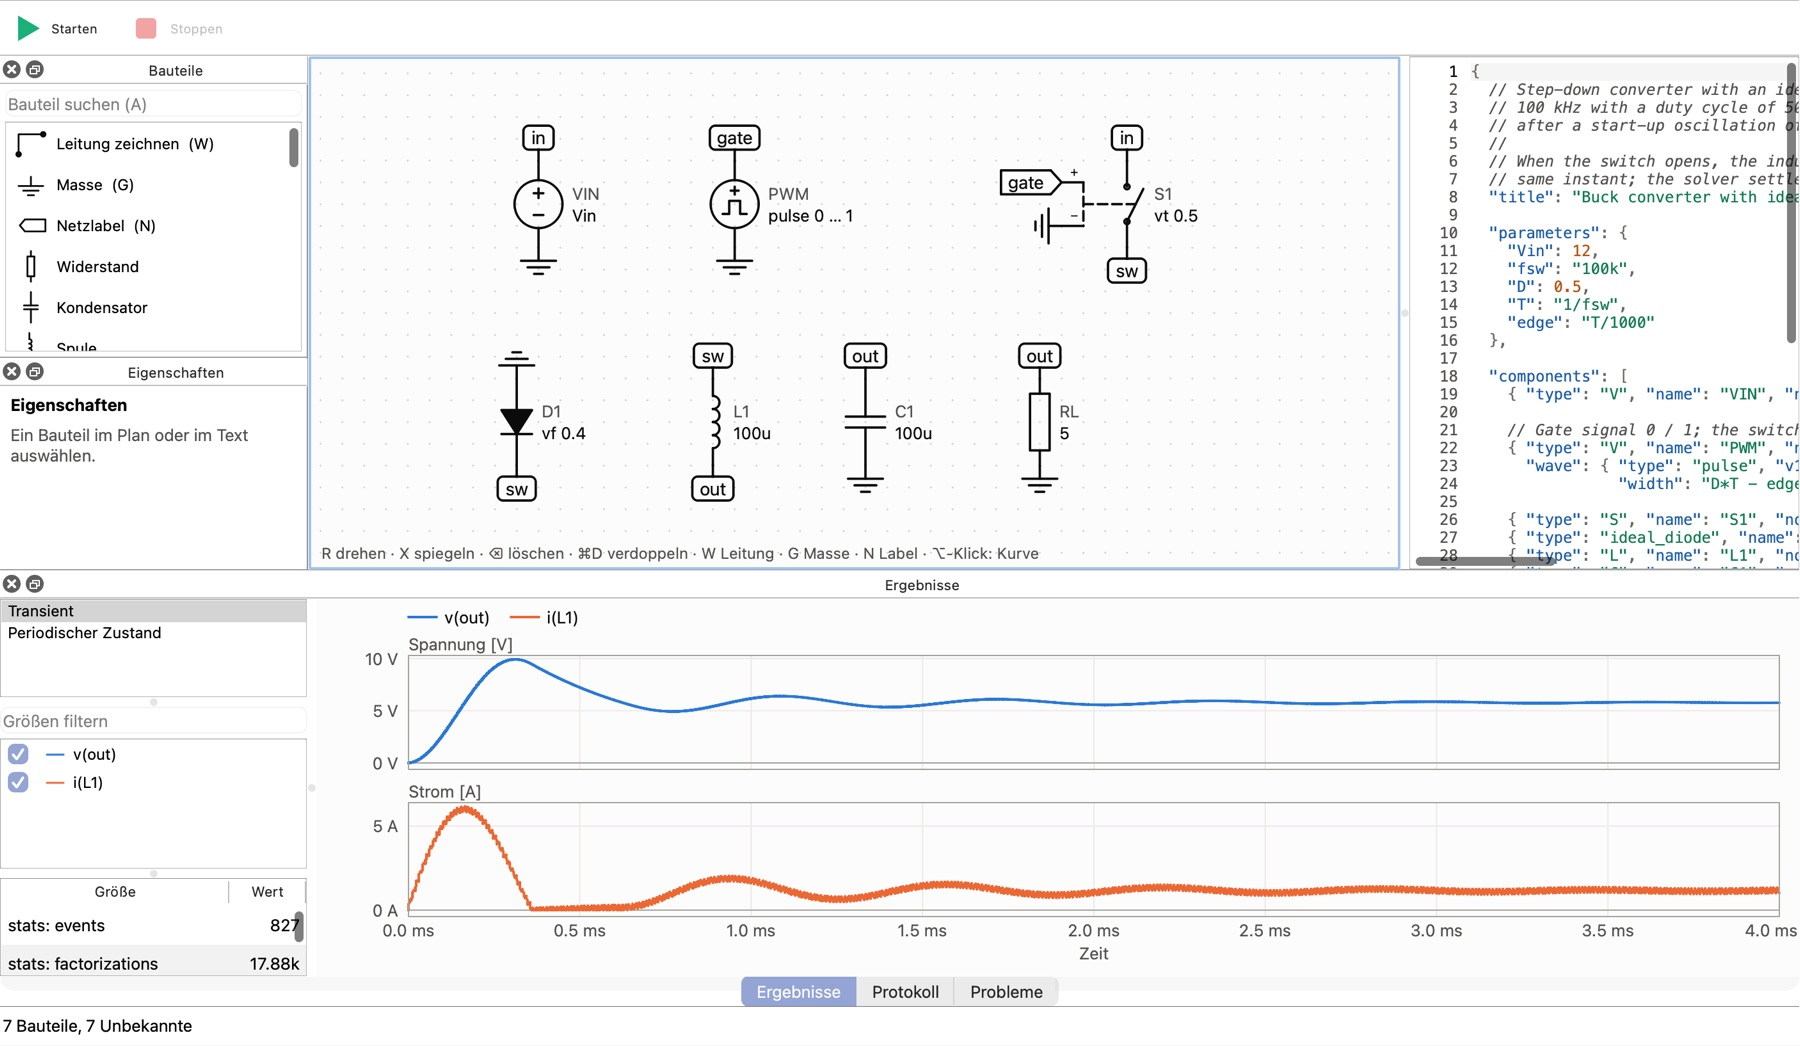
\includegraphics[width=\textwidth]{buck_converter.jpg}
  \caption{Tiefsetzsteller mit idealem Schalter und idealer Diode
    (\code{examples/buck_converter.json}): Einschwingen von
    Ausgangsspannung und Spulenstrom, 827 Schaltereignisse.}
  \label{abb:buck}
\end{figure}

\section{Leitungen T}
\label{sec:leitung}

\begin{json}
{ "type": "T", "name": "T1", "nodes": ["a", "0", "b", "0"], "z0": 50, "td": "5n" },
{ "type": "T", "name": "T2", "nodes": ["c", "0", "d", "0"],
  "l": "250n", "c": "100p", "r": 0.2, "g": 0, "len": 3 }
\end{json}

\begin{itemize}
  \item \textbf{Verlustlos}: Wellenwiderstand \code{z0} und Laufzeit
    \code{td}; alternativ wie in SPICE \code{f} und \code{nl} (Laufzeit
    $= \mathit{nl}/f$), oder Induktivitätsbelag \code{l} und
    Kapazitätsbelag \code{c} je Länge mit der Länge \code{len}.
  \item In der Zeitsimulation wird die Vorgeschichte der Wellen an beiden
    Toren gespeichert; kein Schritt ist länger als \code{td}, und Flanken
    setzen an ihrer Ankunftszeit einen Haltepunkt. Im Arbeitspunkt ist die
    Leitung eine Verbindung, in der AC-Analyse wirkt die Laufzeit exakt als
    Phasendrehung.
  \item \textbf{Verlustbehaftet}: Mit Längswiderstand \code{r} und
    Querleitwert \code{g} je Länge wird die Leitung in verlustlose
    Abschnitte geteilt, zwischen denen die Verluste sitzen. Die Laufzeit
    bleibt exakt; der Fehler fällt mit dem Quadrat der Abschnittszahl. Ohne
    \code{segments} wird sie so gewählt, dass auf jeden Abschnitt höchstens
    ein Zehntel von $Z_0$ entfällt. Der Skineffekt ist nicht modelliert.
  \item \code{i(T1)} ist der Strom in Tor~1.
\end{itemize}

\section{Halbleiter}

Dioden, Bipolartransistoren, JFETs und MOSFETs bekommen ihre Parameter
entweder direkt am Bauteil oder über \code{"model": "<Name>"} aus
\code{models}; Angaben am Bauteil überschreiben das Modell:

\begin{json}
{ "type": "M", "name": "M1", "nodes": ["d", "g", "0", "0"], "model": "n18",
  "w": "2u", "l": "0.18u" }
\end{json}

Die Polarität eines Transistors folgt aus dem \code{type} des Bauteils
(\code{npn}, \code{pmos}, \dots) oder des Modells. Ein MOSFET mit drei Knoten
hat seinen Bulk an der Source. Die Modelle beschreibt
Kapitel~\ref{kap:format-modelle}.

\chapter{Halbleitermodelle}
\label{kap:format-modelle}

\section{Modelle angeben}

Modellparameter stehen unter \code{models} und werden über \code{"model"}
am Bauteil benutzt. Ein Modell kann ein JSON-Objekt sein:

\begin{json}
"models": {
  "DGEN": { "type": "diode", "is": 2.5e-9, "n": 1.75, "cj0": "4p", "tt": "20n" },
  "nch":  { "type": "nmos", "vto": 0.7, "kp": "120u", "lambda": 0.05, "tox": "8n" }
}
\end{json}

oder eine SPICE-Zeile, wie sie Hersteller veröffentlichen; lange Karten als
Liste ihrer Zeilen:

\begin{json}
"models": {
  "QGEN": ".model QGEN NPN(Is=1e-14 Bf=200 Br=2 Vaf=100 Ikf=0.3 Rb=10 Rc=1 Cje=10p Cjc=5p Tf=0.5n Tr=50n)",
  "n18":  [".model n18 NMOS (LEVEL=49 TOX=4.1E-9 VTH0=0.369",
           "+ K1=0.579 U0=293 VSAT=1.68E5 ...)"]
}
\end{json}

In SPICE-Zeilen gelten die SPICE-Regeln: Groß- und Kleinschreibung egal,
\code{m} und \code{M} sind Milli, \code{meg} ist Mega. Unterstützt werden die
Typen \code{D}, \code{NPN}, \code{PNP}, \code{NMOS}, \code{PMOS},
\code{NJF}, \code{PJF}. Parameter, die esim kennt, aber nicht auswertet
(etwa Angaben für Gehäuse oder Rauschmodelle anderer Simulatoren), werden
einmal aufgelistet und übergangen. Ausdrücke in geschweiften Klammern
(\code{KF={PWR(FLW,0.5)/1E11}}) werden mit den Parametern ausgewertet.

Die Namen und Standardwerte der Parameter folgen SPICE. Die folgenden
Tabellen nennen alle Parameter mit ihren Standardwerten.

\section{Diode}

Shockley-Gleichung mit Bahnwiderstand, Sperrschicht- und
Diffusionskapazität und Durchbruch für Z-Dioden.

\begin{longtable}{@{}lP{8.2cm}ll@{}}
  \toprule
  Parameter & Bedeutung & Einheit & Standard \\
  \midrule
  \endhead
  \bottomrule
  \endfoot
  \code{is} & Sättigungsstrom & A & $10^{-14}$ \\
  \code{n} & Emissionskoeffizient & – & 1 \\
  \code{rs} & Bahnwiderstand & \ohm & 0 \\
  \code{cj0} & Sperrschichtkapazität bei 0\,V & F & 0 \\
  \code{vj} & Diffusionsspannung & V & 1 \\
  \code{m} & Gradationsexponent & – & 0,5 \\
  \code{fc} & Grenze der Sperrschichtformel in Flussrichtung & – & 0,5 \\
  \code{tt} & Transitzeit (Diffusionsladung) & s & 0 \\
  \code{bv} & Durchbruchspannung & V & $\infty$ \\
  \code{ibv} & Strom bei der Durchbruchspannung & A & $10^{-3}$ \\
  \code{eg} & Bandabstand (Temperaturgang von \code{is}) & eV & 1,11 \\
  \code{xti} & Temperaturexponent von \code{is} & – & 3 \\
  \code{kf}, \code{af} & 1/f-Rauschen: Koeffizient, Exponent & – & 0, 1 \\
\end{longtable}

\section{Bipolartransistor}

Gummel-Poon-Modell mit Early-Effekt, Hochstromabfall der Verstärkung,
Leckströmen, Bahnwiderständen sowie Sperrschicht- und Diffusionsladungen.
Nicht enthalten sind die Substratdiode, der stromabhängige Basiswiderstand
und die Arbeitspunktabhängigkeit der Transitzeit (\code{xtf}, \code{vtf},
\code{itf}).

\begin{longtable}{@{}lP{8.2cm}ll@{}}
  \toprule
  Parameter & Bedeutung & Einheit & Standard \\
  \midrule
  \endhead
  \bottomrule
  \endfoot
  \code{is} & Transportsättigungsstrom & A & $10^{-16}$ \\
  \code{bf}, \code{br} & Stromverstärkung vorwärts, rückwärts & – & 100, 1 \\
  \code{nf}, \code{nr} & Emissionskoeffizienten & – & 1, 1 \\
  \code{vaf}, \code{var} & Early-Spannung vorwärts, rückwärts & V & $\infty$ \\
  \code{ikf}, \code{ikr} & Kniestrom der Hochstrominjektion & A & $\infty$ \\
  \code{ise}, \code{ne} & Leckstrom Basis–Emitter: Sättigungsstrom, Emissionskoeffizient & A, – & 0, 1,5 \\
  \code{isc}, \code{nc} & Leckstrom Basis–Kollektor & A, – & 0, 2 \\
  \code{rb}, \code{rc}, \code{re} & Bahnwiderstände & \ohm & 0 \\
  \code{cje}, \code{vje}, \code{mje} & Sperrschicht Basis–Emitter: Kapazität, Potential, Exponent & F, V, – & 0, 0,75, 0,33 \\
  \code{cjc}, \code{vjc}, \code{mjc} & Sperrschicht Basis–Kollektor & F, V, – & 0, 0,75, 0,33 \\
  \code{tf}, \code{tr} & Transitzeit vorwärts, rückwärts & s & 0 \\
  \code{fc} & Grenze der Sperrschichtformel & – & 0,5 \\
  \code{eg}, \code{xti} & Bandabstand, Temperaturexponent von \code{is} & eV, – & 1,11, 3 \\
  \code{xtb} & Temperaturexponent der Stromverstärkung & – & 0 \\
  \code{kf}, \code{af} & 1/f-Rauschen des Basisstroms & – & 0, 1 \\
\end{longtable}

\section{Sperrschicht-FET}

Shichman-Hodges-Modell (quadratische Kennlinie, Kanallängenmodulation) mit
Sperrschichten am Gate und deren Kapazitäten. \code{vto} ist für beide
Polaritäten negativ angegeben.

\begin{longtable}{@{}lP{8.2cm}ll@{}}
  \toprule
  Parameter & Bedeutung & Einheit & Standard \\
  \midrule
  \endhead
  \bottomrule
  \endfoot
  \code{vto} & Abschnürspannung & V & $-2$ \\
  \code{beta} & Steilheitsparameter & A/V$^2$ & $10^{-4}$ \\
  \code{lambda} & Kanallängenmodulation & 1/V & 0 \\
  \code{is} & Sättigungsstrom der Gate-Dioden & A & $10^{-14}$ \\
  \code{cgs}, \code{cgd} & Gate-Kapazitäten bei 0\,V & F & 0 \\
  \code{pb} & Potential der Gate-Sperrschicht & V & 1 \\
  \code{fc} & Grenze der Sperrschichtformel & – & 0,5 \\
  \code{kf}, \code{af} & 1/f-Rauschen & – & 0, 1 \\
\end{longtable}

\section{MOSFET}

Für MOSFETs gibt es vier Modelle, gewählt mit \code{level}:

\begin{center}
\begin{tabularx}{\textwidth}{@{}lL@{}}
  \toprule
  \code{level} & Modell \\
  \midrule
  1 (Standard) & Shichman-Hodges: einfach, robust, für Übungen und digitale Grundschaltungen \\
  \code{"ekv"} & ladungsbasiert, glatt von schwacher bis starker Inversion \\
  3 & SPICE MOS3: halbempirisches Kurzkanalmodell, verbreitet bei Leistungs-MOSFETs \\
  \code{"bsim3"} (SPICE 8, 49, 53) & BSIM3v3.3: Kurzkanalmodell der Halbleiterprozesse \\
  \bottomrule
\end{tabularx}
\end{center}

\subsection{Level 1}

Shichman-Hodges mit Substrateffekt, Kanallängenmodulation, Bulk-Dioden,
Überlapp- und Sperrschichtkapazitäten. Mit \code{tox} kommt die Ladung des
Kanals hinzu: ladungserhaltend, in Sättigung 40\,:\,60 auf Drain und Source
verteilt, Gate-Kapazität $\frac23 C_\text{ox}$ in Sättigung und
$C_\text{ox}$ im Widerstandsbereich und unterhalb der Schwelle.

\begin{longtable}{@{}lP{8.2cm}ll@{}}
  \toprule
  Parameter & Bedeutung & Einheit & Standard \\
  \midrule
  \endhead
  \bottomrule
  \endfoot
  \code{vto} & Schwellspannung (negativ beim selbstsperrenden P-MOSFET) & V & 0 \\
  \code{kp} & Steilheitsparameter $\mu C_\text{ox}$ & A/V$^2$ & $2\cdot10^{-5}$ \\
  \code{gamma} & Substratsteuerfaktor & $\sqrt{\text{V}}$ & 0 \\
  \code{phi} & Oberflächenpotential & V & 0,6 \\
  \code{lambda} & Kanallängenmodulation & 1/V & 0 \\
  \code{w}, \code{l} & Kanalweite und -länge (meist am Bauteil) & m & $10^{-4}$ \\
  \code{tox} & Oxiddicke; 0: keine Kanalladung & m & 0 \\
  \code{cgso}, \code{cgdo} & Überlappkapazität Gate–Source, Gate–Drain je Weite & F/m & 0 \\
  \code{cgbo} & Überlappkapazität Gate–Bulk je Länge & F/m & 0 \\
  \code{cbd}, \code{cbs} & Sperrschichtkapazitäten Bulk–Drain, Bulk–Source & F & 0 \\
  \code{pb}, \code{mj}, \code{fc} & Potential, Exponent, Grenze der Bulk-Sperrschichten & V, –, – & 0,8, 0,5, 0,5 \\
  \code{is} & Sättigungsstrom der Bulk-Dioden & A & $10^{-14}$ \\
  \code{tcv} & Temperaturkoeffizient der Schwellspannung & V/K & 0 \\
  \code{kf}, \code{af} & 1/f-Rauschen & – & 0, 1 \\
\end{longtable}

\subsection{EKV (\texttt{"level": "ekv"})}

Ladungsbasiertes Modell nach Enz, Krummenacher und Vittoz. Ein einziger
glatter Ausdruck beschreibt den Strom von schwacher bis starker Inversion:
Unterhalb der Schwelle fällt er exponentiell ($n V_T \ln 10$ je Dekade, $n$
aus \code{gamma}), weit darüber gilt das Quadratgesetz von Level~1. Dazu
kommen Beweglichkeitsreduktion durch das Gate-Feld (\code{theta} in 1/V),
Geschwindigkeitssättigung (\code{ucrit} in V/m, wirkt mit der Kanallänge)
und Kanallängenmodulation (\code{lambda}). Das Modell ist symmetrisch in
Drain und Source, alle Ableitungen sind stetig, und die Ladungen (mit
\code{tox}) stammen aus demselben Ansatz.

Es ersetzt kein BSIM: Kurzkanaleffekte wie DIBL oder Gate-Ströme fehlen.
Wo Level~1 unterhalb der Schwelle exakt 0 liefert (Leckströme, Schaltungen
im Unterschwellbetrieb, Analogschalter nahe 0\,V), ist es die bessere Wahl;
\datei{examples/mosfet_subthreshold.json} vergleicht beide.

\subsection{Level 3}

Das halbempirische Kurzkanalmodell von SPICE (MOS3), das viele
Herstellermodelle von MOSFETs benutzen, etwa die von Transim erzeugten
Modelle von Leistungs-MOSFETs. Zusätzlich zu den Parametern von Level~1:

\begin{longtable}{@{}lP{8.2cm}ll@{}}
  \toprule
  Parameter & Bedeutung & Einheit & Standard \\
  \midrule
  \endhead
  \bottomrule
  \endfoot
  \code{theta} & Beweglichkeitsreduktion durch das Gate-Feld & 1/V & 0 \\
  \code{eta} & statische Rückwirkung (Absenkung der Schwelle durch den Drain) & – & 0 \\
  \code{vmax} & maximale Driftgeschwindigkeit; 0: keine Sättigung & m/s & 0 \\
  \code{nfs} & Dichte schneller Oberflächenzustände; $>0$: Strom unterhalb der Schwelle & 1/cm$^2$ & 0 \\
  \code{kappa} & Sättigungsfeldfaktor (Kanallängenmodulation, mit \code{nsub}) & – & 0,2 \\
  \code{xj} & Tiefe der Übergänge (Kurzkanaleffekt, mit \code{nsub}) & m & 0 \\
  \code{ld} & seitliche Diffusion: wirksame Länge $l - 2\,\mathit{ld}$ & m & 0 \\
  \code{delta} & Weiteneffekt auf die Schwelle & – & 0 \\
  \code{u0} & Oberflächenbeweglichkeit & cm$^2$/Vs & 600 \\
  \code{nsub} & Substratdotierung; 0: nicht angegeben & 1/cm$^3$ & 0 \\
  \code{nss} & Dichte der Oberflächenzustände (Schwelle aus \code{nsub}) & 1/cm$^2$ & 0 \\
  \code{tpg} & Art des Gate-Materials (Schwelle aus \code{nsub}) & – & 1 \\
\end{longtable}

Ohne \code{kp} folgt es aus \code{u0} und \code{tox}; ohne \code{tox} gilt
$10^{-7}$\,m; aus \code{nsub} folgen fehlende \code{gamma}, \code{phi} und
\code{vto}. Der Temperaturgang ist der von ngspice. Der Drainstrom stimmt
mit ngspice (MOS3) auf besser als $10^{-9}$ überein. Die Gate-Ladung ist
die ladungserhaltende von Level~1 mit der Schwellspannung von Level~3
(ngspice rechnet hier mit Kapazitäten nach Meyer), was Schaltflanken leicht
verändert.

\subsection{BSIM3 (\texttt{"level": "bsim3"})}

Der Drainstrom nach BSIM3v3.3, dem Kurzkanalmodell, für das
Halbleiterhersteller Parametersätze veröffentlichen; in SPICE-Karten als
\code{LEVEL=8}, \code{49} oder \code{53}. Umgesetzt sind:

\begin{itemize}
  \item Schwellspannung mit Kurz- und Schmalkanaleffekten und DIBL,
    Unterschwellstrom,
  \item die drei Beweglichkeitsmodelle, Geschwindigkeitssättigung,
    Bahnwiderstände,
  \item Kanallängenmodulation, DIBL und SCBE im Ausgangsleitwert,
    Poly-Verarmung, Substratstrom,
  \item Temperaturabhängigkeit und die Größenabhängigkeit aller Parameter
    über ihre L-, W- und P-Varianten,
  \item die Kapazitätsmodelle \code{capmod} 0 bis 3 (Standard 3): 0
    stückweise mit eigener Flachbandspannung \code{vfbcv}, 1 und 2 mit
    \code{vfbzb} aus der Schwellspannung (2 mit glatten Übergängen), 3 das
    Charge-Thickness-Modell (\code{acde}, \code{moin}),
  \item die Aufteilung der Kanalladung mit \code{xpart} (0: 40/60, 0,5:
    50/50, 1: 0/100, negativ: keine Kanalladung), dazu \code{noff},
    \code{voffcv}, \code{clc}, \code{cle}, \code{dlc}, \code{dwc} mit
    \code{llc} \dots{} \code{wwlc} und die spannungsabhängigen
    Überlappkapazitäten \code{cgsl}, \code{cgdl}, \code{ckappa},
  \item Sperrschichtkapazitäten (\code{cj}, \code{cjsw}, \code{cjswg}) mit
    den Instanzparametern \code{ad}, \code{as}, \code{pd}, \code{ps}, sowie
    \code{w}, \code{l} und der Zahl paralleler Transistoren \code{m}.
\end{itemize}

Es gelten die Gleichungen ab BSIM3v3.2: \code{capmod} 1 und 2 nehmen
\code{vfbzb}, auch wenn die Karte \code{VERSION=3.1} angibt. Es fehlen die
Rauschmodelle von BSIM3 (es gelten die Formeln von Level~1),
nicht-quasistatische Effekte (\code{nqsmod}, \code{elm}) und die Auswahl
zwischen mehreren Karten nach \code{lmin}/\code{lmax}. Parameter, die
deshalb ohne Wirkung bleiben, werden still akzeptiert; unbekannte werden
gemeldet.

Geprüft sind Drainstrom und Ladungen gegen eine getrennt geschriebene
Umsetzung derselben Gleichungen in Python (16 bzw. 25 Parametersätze mit je
über 600 Arbeitspunkten, Übereinstimmung auf $5\cdot10^{-9}$ bzw.
$10^{-8}$) und gegen BSIM3v3.3 in ngspice (Übereinstimmung auf
$10^{-9}$). Ein Beispiel ist \datei{examples/ring_oscillator_bsim3.json}.

\section{Temperatur}
\label{sec:temperatur}

\code{options.temp} ist die Temperatur der Schaltung, \code{options.tnom}
(Standard 27\,°C) die, für die die Modellparameter gelten. Skaliert werden
die Sättigungsströme aller pn-Übergänge (\code{eg}, \code{xti}), die
Stromverstärkung von Bipolartransistoren (\code{xtb}), die Beweglichkeit im
MOSFET ($k_p \sim T^{-1{,}5}$) und auf Wunsch die Schwellspannung
(\code{tcv} in V/K). Sperrschichtpotentiale und Kapazitäten bleiben bei
Level~1 unverändert; Level~3 und BSIM3 haben ihren eigenen, vollständigeren
Temperaturgang.

Eine Analyse bei mehreren Temperaturen ist ein Parameter-Sweep über einen
Parameter, der in \code{options.temp} steht:

\begin{json}
"parameters": { "T": 27 },
"options": { "temp": "T" },
"analyses": [ { "type": "dc", "source": "V1", "start": 0, "stop": 0.8, "step": 0.01,
                "param_sweep": { "param": "T", "values": [-40, 27, 125] } } ]
\end{json}

\chapter{Teilschaltungen}
\label{kap:format-teilschaltungen}

\section{Definition und Instanz}

Wiederverwendbare Teilschaltungen stehen unter \code{subcircuits} und
werden mit dem Bauteil \code{X} eingesetzt:

\begin{json}
"subcircuits": {
  "divider": {
    "ports": ["in", "out"],
    "parameters": { "ratio": 0.5, "rtotal": "10k" },
    "components": [
      { "type": "R", "name": "R1", "nodes": ["in", "out"], "value": "(1 - ratio)*rtotal" },
      { "type": "R", "name": "R2", "nodes": ["out", "0"],  "value": "ratio*rtotal" }
    ]
  }
},
"components": [
  { "type": "X", "name": "X1", "subcircuit": "divider", "nodes": ["a", "b"] },
  { "type": "X", "name": "X2", "subcircuit": "divider", "nodes": ["a", "c"],
    "parameters": { "ratio": 0.25 } }
]
\end{json}

\begin{description}[style=nextline,leftmargin=2em]
  \item[Knoten]
    Die Namen in \code{ports} stehen für die außen angeschlossenen Knoten,
    in der Reihenfolge der \code{nodes} der Instanz. Alle anderen Knoten
    sind lokal. Masse (\code{"0"}) ist überall dieselbe.
  \item[Parameter]
    \code{parameters} der Definition enthält Standardwerte; sie dürfen sich
    auf globale Parameter und aufeinander beziehen. Die Instanz
    überschreibt einzelne Werte mit \code{"parameters": {...}}.
  \item[Inhalt]
    Alle Bauteile, auch weitere Instanzen (Schachtelung bis 20 Ebenen),
    dazu eigene \code{models}, \code{variables}, \code{equations} und
    \code{events}. Ein Bauteil mit thermischem Zustand oder eigener
    Kennlinie lässt sich so als Modell kapseln und mehrfach verwenden.
  \item[Plan]
    Der Editor legt den Plan der Teilschaltung unter \code{"schematic"} in
    ihrer Definition ab.
\end{description}

\section{Namen von außen}

Was in der Instanz \code{X1} liegt, heißt außen \code{X1.<Name>}, bei
Schachtelung \code{X1.U.<Name>}:

\begin{itemize}
  \item Knotenspannungen: \code{v(X1.mid)},
  \item Ströme: \code{i(X1.V1)},
  \item Variablen: \code{X1.T},
  \item Quellen eines DC-Sweeps: \code{"source": "X1.V1"}.
\end{itemize}

Innerhalb einer Teilschaltung beziehen sich \code{i(...)} und
\code{control} auf Bauteile derselben Teilschaltung. In der Standardausgabe
(ohne \code{outputs}) erscheint das Innere von Instanzen nicht; innere
Größen müssen ausdrücklich unter \code{outputs} stehen.

\section{Teilschaltungen in SPICE}
\label{sec:spice-subckt}

Modelle der Hersteller lassen sich unverändert einsetzen: Statt eines
Objekts steht der SPICE-Text, als eine Zeichenkette oder als Liste von
Zeilen.

\begin{json}
"subcircuits": {
  "OPX": [
    ".SUBCKT OPX inp inn out vp vn",
    "Rin inp inn 1meg",
    "Egain mid 0 POLY(1) inp inn 0 1e5",
    "Rout mid out 10",
    "Dhi out vp DCLAMP",
    "Dlo vn out DCLAMP",
    ".MODEL DCLAMP D(IS=1e-14)",
    ".ENDS"
  ]
},
"components": [
  { "type": "X", "name": "U1", "subcircuit": "OPX", "nodes": ["in", "fb", "out", "vp", "vn"] }
]
\end{json}

Die Modellbibliothek des Editors erzeugt genau diese Form
(Kapitel~\ref{kap:editor-bibliothek}).

\subsection*{Was gelesen wird}

\begin{itemize}
  \item Bauteile \code{R}, \code{C}, \code{L}, \code{K}, \code{V} und
    \code{I} (DC, AC, SIN, PULSE, PWL), \code{E} und \code{G} (linear,
    \code{POLY(n)}, \code{VALUE = {...}}, \code{TABLE {...} = (x, y) ...}),
    \code{F} und \code{H} (linear, \code{POLY(n)}), \code{B} (\code{V=}
    oder \code{I=}), \code{D}, \code{Q}, \code{M}, \code{J}, \code{S},
    \code{T} und \code{X}.
  \item \code{.param}, \code{PARAMS:} an \code{.subckt} und an Instanzen,
    \code{.model} – auch mit Ausdrücken, ausgewertet mit den Parametern der
    Teilschaltung.
  \item Formen von PSpice: Widerstände mit Modell (\code{R1 a b RMOD 1k};
    \code{R=} im Modell skaliert, \code{T_ABS=-273.15} macht den Widerstand
    rauschfrei); Schalter mit \code{VSWITCH(RON ROFF VON VOFF)} mit dem
    stetigen Übergang von PSpice zwischen \code{VOFF} und \code{VON}
    (intern eine Verhaltensquelle); Schalter mit \code{SW(VT VH)} werden
    esims Schalter mit Hysterese.
  \item Ausdrücke in \code{{...}}: Zahlen mit SPICE-Endungen (\code{M} ist
    Milli, \code{meg} Mega), \code{**}, \code{a ? b : c}, \code{limit},
    \code{pwr}, \code{pwrs}, \code{uramp}, \code{u}, \code{stp},
    \code{sgn}.
\end{itemize}

Modelle und weitere \code{.subckt} im Text gehören zu dieser
Teilschaltung und heißen intern \code{OPX/NAME}; sie stoßen nicht mit
Modellen der Datei zusammen. Was der Text nicht definiert, sucht esim in
der Datei.

\subsection*{Was nicht geht}

Nicht Unterstütztes (z.\,B. \code{LAPLACE}, \code{.include}, unbekannte
Bauteile) ist ein Fehler, der die Zeile im Text nennt. Ohne Wirkung
bleiben, mit Warnung, etwa die Fläche von Dioden und der Substratknoten
von Transistoren.

\subsection*{Erprobt}

\begin{itemize}
  \item Das Makromodell eines verbreiteten Doppel-Operationsverstärkers
    (PSpice, 18 Teilschaltungen, 227 Bauteile): DC-Kennlinie und
    Sprungantwort stimmen mit ngspice im PSpice-Modus überein (DC auf 7
    Stellen, Zeitverlauf auf 0,3\,mV).
  \item Ein kleiner P-Kanal-MOSFET als Level-3-Modell eines Herstellers:
    Kennlinien wie ngspice auf 6 Stellen, Schaltflanke auf 17\,mV bei 5\,V
    Hub.
  \item \datei{tests/spice_subckt_ngspice.py} vergleicht eine SPICE-
    Teilschaltung mit allen Formen dieses Abschnitts gegen ngspice.
\end{itemize}

\chapter{Analysen}
\label{kap:format-analysen}

\section{Übersicht}

Die Liste \code{analyses} nennt die Analysen; sie werden in dieser
Reihenfolge gerechnet.

\begin{center}
\begin{tabularx}{\textwidth}{@{}lP{5.6cm}L@{}}
  \toprule
  \code{type} & Parameter & Ergebnis \\
  \midrule
  \code{op} & – & Arbeitspunkt (Konsole) \\
  \code{dc} & \code{source}, \code{start}, \code{stop}, \code{step} & Sweep einer V- oder I-Quelle \\
  \code{ac} & \code{sweep}, \code{points}, \code{fstart}, \code{fstop} & Betrag und Phase je Ausgang \\
  \code{tran} & \code{tstop}, optional \code{tstep}, \code{method}, \code{uic}, \code{output_step}, \dots & Zeitverlauf \\
  \code{noise} & \code{output}, \code{input}, Frequenzen wie \code{ac} & Rauschdichten \\
  \code{pss} & \code{period}, optional \code{periods}, \code{tstab}, \code{tol} & eingeschwungene Periode \\
  \code{sens} & \code{analysis}, optional \code{parameters}, \code{delta} & Empfindlichkeiten \\
  \code{fit} & \code{analysis}, \code{output}, \code{data}, \code{parameters} & angepasste Parameter \\
  \bottomrule
\end{tabularx}
\end{center}

Für jede Analyse gilt außerdem:

\begin{itemize}
  \item \code{"name"} gibt ihr einen eigenen Namen (für die Ergebnisdatei
    und für Python); ohne Namen heißt sie wie ihr Typ.
  \item \code{"outputs"} ersetzt für diese Analyse die globale Liste der
    Ausgänge.
  \item \code{"measure"} berechnet Kennwerte aus den Kurven
    (Abschnitt~\ref{sec:messgroessen}).
  \item \code{"param_sweep"} und \code{"monte_carlo"} wiederholen sie
    (Kapitel~\ref{kap:format-studien}).
  \item \code{"save": false} unterdrückt die Datei mit den Kurven, wenn nur
    Messgrößen interessieren.
\end{itemize}

\section{Arbeitspunkt (op)}

\begin{json}
{ "type": "op" }
\end{json}

Der Arbeitspunkt ist die stationäre Lösung: Kondensatoren sind offen,
Spulen kurzgeschlossen, Quellen stehen auf ihrem \code{dc}-Wert,
Zeitableitungen eigener Gleichungen sind null. Die Werte der Ausgänge
erscheinen auf der Konsole. Konvergiert das Newton-Verfahren nicht direkt,
versucht esim nacheinander eine Pseudo-Transiente, gmin-Stepping und
Quellen-Stepping (Kapitel~\ref{kap:numerik}); die Konsole nennt, welches
Verfahren zum Ziel geführt hat. Bei bistabilen Schaltungen wählt
\code{"nodeset"} den gewünschten Zustand (Abschnitt~\ref{sec:optionen}).

\section{DC-Sweep (dc)}

\begin{json}
{ "type": "dc", "source": "Vin", "start": 0, "stop": 5, "step": 0.01 }
\end{json}

Der Wert der Quelle \code{source} (Spannungs- oder Stromquelle, auch in
einer Teilschaltung: \code{"X1.V1"}) läuft von \code{start} bis \code{stop}
in Schritten von \code{step}; für jeden Wert wird der Arbeitspunkt
bestimmt, ausgehend vom vorigen. Die erste Spalte der Ergebnisdatei ist der
Wert der Quelle. Übertragungskennlinien, Ausgangskennlinienfelder (mit einem
Parameter-Sweep außen herum) und Kennlinien von Bauteilen entstehen so.

\section{Frequenzgang (ac)}

\begin{json}
{ "type": "ac", "sweep": "dec", "points": 20, "fstart": 10, "fstop": "10meg" }
\end{json}

Die Kleinsignalanalyse linearisiert die Schaltung im Arbeitspunkt und
rechnet für jede Frequenz das komplexe lineare Gleichungssystem. Angeregt
wird sie von den Quellen mit \code{ac} (und \code{acphase}).

\begin{itemize}
  \item \code{sweep}: \code{"dec"} (Standard; \code{points} je Dekade),
    \code{"oct"} (je Oktave) oder \code{"lin"} (\code{points} insgesamt).
    \code{points} ist ohne Angabe 10.
  \item Die Ergebnisdatei enthält je Ausgang \code{mag(...)} (Betrag) und
    \code{phase(...)} (Grad). Der Editor zeigt den Betrag in dB.
  \item Nur einfache Ausgänge sind erlaubt: \code{v(knoten)},
    \code{v(a,b)}, \code{i(bauteil)}, Variablen.
  \item Eigene Gleichungen und Verhaltensquellen sind in der
    Linearisierung enthalten. Die Laufzeit von Leitungen wirkt exakt als
    Phasendrehung; \code{delay(x, td)} in Ausdrücken ist in der
    AC-Analyse dagegen gleich \code{x}.
\end{itemize}

\section{Zeitverlauf (tran)}
\label{sec:tran}

\begin{json}
{ "type": "tran", "tstop": "5m", "tstep": "10u" }
\end{json}

\begin{longtable}{@{}lP{10.6cm}@{}}
  \toprule
  Schlüssel & Bedeutung \\
  \midrule
  \endhead
  \bottomrule
  \endfoot
  \code{tstop} & Endzeit. \\
  \code{tstep} & Gewünschte Auflösung: Kein Schritt wird länger (Standard \code{tstop/50}). \\
  \code{hmax} & Größte Schrittweite (wie \code{tstep}, nur ohne Bezug zur Ausgabe). \\
  \code{hinit}, \code{hmin} & Erste und kleinste Schrittweite. \\
  \code{method} & Integrationsverfahren: \code{"bdf"} (Standard), \code{"gear2"}, \code{"trap"}, \code{"be"}. \\
  \code{max_order} & Höchste Ordnung von \code{"bdf"} (1 bis 5, Standard 5). \\
  \code{uic} & \code{true}: ohne Arbeitspunkt von den Anfangsbedingungen starten. \\
  \code{output_step} & Ausgabe auf dem festen Raster 0, $\Delta t$, $2\Delta t$, \dots \\
  \code{max_events} & Höchstzahl von Ereignissen (Standard 100\,000). \\
  \code{fourier} & Fourier-Analyse am Ende (Abschnitt~\ref{sec:fourier}). \\
\end{longtable}

\paragraph{Start.}
Die Schaltung beginnt in ihrem Arbeitspunkt (mit den Werten der Quellen bei
$t=0$), Zustände eigener Gleichungen bei ihren Anfangswerten
(Abschnitt~\ref{sec:anfangswerte}). Mit \code{"uic": true} wird die
Anfangslösung übersprungen: Es gelten \code{ic} an Kondensatoren und
Spulen, \code{"ic": {"knoten": spannung}} auf oberster Ebene und die
Startwerte der Variablen. Knoten, die Spannungsquellen von Masse aus
festlegen (Versorgungen, auch über Strommesser hinweg), starten auf deren
Spannung; alles andere bei 0.

\paragraph{Schrittweite.}
Die Schrittweite wird automatisch aus dem geschätzten Fehler gewählt
(Abschnitt~\ref{sec:genauigkeit}). Ecken der Quellen (Pulsflanken,
PWL-Stützstellen), Ereignisse und Laufzeiten von Leitungen und Totzeiten
werden exakt getroffen. Sinusquellen begrenzen den Schritt auf ein
Zwanzigstel ihrer Periode.

\paragraph{Verfahren.}
\begin{description}[style=nextline,leftmargin=2em]
  \item[\code{bdf} (Standard)]
    BDF mit variabler Ordnung 1 bis 5. Nach jedem Schritt wird die
    Ordnung gewählt, die den größten nächsten Schritt erlaubt. Bei glatten
    Lösungen und engen Toleranzen braucht es ein Vielfaches weniger
    Schritte als ein Verfahren fester Ordnung.
  \item[{\code{gear2}}]
    BDF fester Ordnung 2. Robust, klingelt nicht, dämpft Schwingungen
    leicht.
  \item[{\code{trap}}]
    Trapezregel. Keine numerische Dämpfung – die beste Wahl für schwach
    gedämpfte Schwingkreise über viele Perioden. Dafür können Ströme von
    Spannungsquellen von Schritt zu Schritt leicht alternieren.
  \item[{\code{be}}]
    Rückwärts-Euler: erste Ordnung, sehr robust, stark dämpfend.
\end{description}

\paragraph{Ausgabe.}
Ohne \code{output_step} wird jeder Zeitpunkt des Lösers ausgegeben; die
Abstände sind dann ungleich. Mit \code{output_step} wird auf ein festes
Raster interpoliert, was für die Weiterverarbeitung (FFT, Vergleich mit
Messungen) praktisch ist; die Schrittweite des Lösers bleibt dabei frei.
Am Zeitpunkt eines Ereignisses steht der Zustand \emph{vor} der Zuweisung,
im Punkt unmittelbar danach der neue.

\section{Fourier-Analyse}
\label{sec:fourier}

\begin{json}
{ "type": "tran", "tstop": "5m", "tstep": "10u",
  "fourier": { "freq": "1k", "harmonics": 9, "outputs": ["v(out)"] } }
\end{json}

Der Block \code{fourier} einer Transientenanalyse berechnet das Spektrum
der letzten ganzen Periode(n) zur Grundfrequenz \code{freq}. Das Ergebnis
steht in \datei{<Name>.tran.fourier.csv} (Betrag und Phase je Harmonischer,
Zeile 0 ist der Mittelwert); Grundschwingung und Klirrfaktor erscheinen auf
der Konsole. \code{periods} (Standard 1) wählt die Zahl der ausgewerteten
Perioden, \code{from} den frühesten Zeitpunkt. Die Genauigkeit hängt von der
Auflösung des Zeitverlaufs ab: Für kleine Klirrfaktoren \code{tstep} und
\code{reltol} klein wählen.

\section{Rauschen (noise)}

\begin{json}
{ "type": "noise", "output": "v(out)", "input": "Vin",
  "sweep": "dec", "points": 20, "fstart": 10, "fstop": "100k" }
\end{json}

Berechnet im Arbeitspunkt die spektrale Rauschdichte am Ausgang
(\code{onoise}, bei einer Spannung in V/$\sqrt{\text{Hz}}$) und, wenn eine
Quelle als \code{input} genannt ist, die auf sie bezogene Dichte
(\code{inoise}) samt Verstärkung. Auf der Konsole stehen das über das Band
integrierte Rauschen und die größten Beiträge. \code{output} ist
\code{v(knoten)}, \code{v(a,b)} oder \code{i(bauteil)}.

Rauschquellen sind das thermische Rauschen aller Widerstände (auch der
Bahnwiderstände von Diode und Transistor), das Schrotrauschen von
Dioden-, Kollektor- und Basisstrom, das thermische Kanalrauschen des MOSFET
und 1/f-Rauschen über die Modellparameter \code{kf} und \code{af}.
Schalter, ideale Dioden und Verhaltensquellen rauschen nicht; Widerstände
mit \code{"noise": false} auch nicht.

\section{Periodischer stationärer Zustand (pss)}

Schaltnetzteile, Gleichrichter oder Verstärker mit großen
Koppelkondensatoren brauchen oft Tausende Perioden, bis sie eingeschwungen
sind. Die Analyse \code{pss} sucht den eingeschwungenen Zustand direkt:

\begin{json}
{ "type": "pss", "period": "10u",
  "measure": { "vout": { "avg": "v(out)" }, "ripple": { "pp": "v(out)" } } }
\end{json}

\begin{itemize}
  \item \code{period} ist die Periode der Anregung. Alle Quellen müssen sich
    mit ihr wiederholen; das wird geprüft.
  \item Gesucht wird ein Zustand, der nach einer Periode wieder erreicht
    ist. Jede Iteration rechnet eine Periode und schätzt aus den letzten
    Ergebnissen, wohin die langsamen Vorgänge laufen
    (Anderson-Beschleunigung). Der Tiefsetzsteller aus
    \datei{examples/buck_converter.json} braucht so 5 Perioden statt etwa
    2000.
  \item Ergebnis ist eine Periode im eingeschwungenen Zustand
    (\code{"periods": n} für mehrere); Messgrößen, \code{fourier} und
    \code{output_step} wirken wie bei \code{tran}.
  \item \code{tol} (Standard $10^{-4}$) ist die relative Abweichung, mit
    der sich der Zustand nach einer Periode wiederholen muss;
    \code{max_iterations} begrenzt die Zahl der Iterationen. \code{tstab}
    rechnet vor der Suche eine Zeit lang normal, was bei stark
    nichtlinearem Anlauf hilft.
\end{itemize}

Die Periode muss bekannt sein. Für selbstschwingende Schaltungen
(Oszillatoren) ist die Analyse nicht gedacht, ebenso wenig für Zustände, die
erst nach einem Schaltvorgang mit Gedächtnis erreicht werden (Hysterese,
diskrete Variablen). Totzeiten und Leitungen unterstützt sie nicht.

\section{Empfindlichkeiten (sens)}

Die Analyse \code{sens} beantwortet die Frage, welche Parameter ein
Ergebnis bestimmen:

\begin{json}
{ "type": "sens", "parameters": ["R1", "R2", "C"],
  "analysis": { "type": "ac", "sweep": "dec", "points": 100, "fstart": 1, "fstop": "100k",
                "measure": { "fc": { "f3db": "v(out)" } } } }
\end{json}

\begin{itemize}
  \item Jeder Parameter wird um $\pm$\code{delta} (relativ, Standard
    $10^{-3}$) geändert, die eingebettete Analyse wiederholt und der
    Differenzenquotient gebildet – zwei Rechnungen je Parameter.
  \item Betrachtet werden die Messgrößen der Analyse, bei \code{op} ihre
    Ausgänge.
  \item Ohne \code{parameters} werden alle Einträge von \code{parameters}
    variiert.
  \item Ausgegeben wird die normierte Empfindlichkeit: um wie viel Prozent
    sich das Ergebnis ändert, wenn der Parameter um ein Prozent wächst. Die
    Tabelle steht in \datei{<Name>.sens.csv}; die Zusammenfassung
    (\code{--summary}) enthält zusätzlich die absoluten Ableitungen.
  \item Messgrößen aus abgetasteten Kurven (Grenzfrequenzen,
    Durchgangszeiten) sind nur so genau wie das Raster; dann ein größeres
    \code{delta} (z.\,B. 0,02) oder ein feineres Raster wählen.
\end{itemize}

\section{Anpassung an Messdaten (fit)}

Die Analyse \code{fit} verändert Parameter so, dass eine simulierte Kurve
möglichst gut auf Datenpunkten liegt (kleinste Quadrate nach
Levenberg-Marquardt):

\begin{json}
{ "type": "fit",
  "analysis": { "type": "dc", "source": "V1", "start": 0.25, "stop": 0.75, "step": 0.005 },
  "output": "-i(V1)",
  "data": { "file": "data/diode_iv.csv", "xcol": 0, "ycol": 1 },
  "parameters": { "is0": { "min": 1e-14, "max": 1e-6, "log": true },
                  "n0":  { "min": 1, "max": 3 } },
  "residual": "log" }
\end{json}

\begin{itemize}
  \item \code{analysis} ist eine \code{dc}-, \code{ac}- oder
    \code{tran}-Analyse; \code{output} die Größe, die mit den Daten
    verglichen wird (bei \code{ac} ihr Betrag). Die Daten müssen innerhalb
    des simulierten Bereichs liegen; dazwischen wird linear interpoliert.
  \item \code{data}: \code{x} und \code{y}, \code{points} oder eine Datei
    wie bei den Tabellen (Abschnitt~\ref{sec:tabellen}).
  \item \code{parameters}: je Parameter optional \code{start} (sonst der
    Wert aus \code{parameters}), \code{min}, \code{max} und
    \code{"log": true}, wenn sich der Wert über Größenordnungen bewegen
    kann.
  \item \code{residual}: \code{"lin"} (Differenz, Standard), \code{"rel"}
    (relativ zu den Daten) oder \code{"log"} (Logarithmus des Verhältnisses,
    für Daten über mehrere Dekaden).
  \item Ergebnis: die angepassten Werte und der mittlere Restfehler auf der
    Konsole, Daten und Modellkurve in \datei{<Name>.fit.csv}.
\end{itemize}

Das Verfahren findet ein lokales Minimum; die Startwerte sollten in der
richtigen Größenordnung liegen. Parameter, die die Kurve im gemessenen
Bereich kaum beeinflussen, bleiben unbestimmt.
\datei{examples/fit_diode.json} passt so das Modell einer Diode an eine
gemessene Kennlinie an.

\section{Messgrößen}
\label{sec:messgroessen}

Mit \code{measure} berechnet eine Analyse Kennwerte aus ihren Kurven:

\begin{json}
{ "type": "tran", "tstop": "200m",
  "measure": {
    "vdc":    { "avg": "v(out)", "from": "160m" },
    "ripple": { "pp":  "v(out)", "from": "160m" },
    "t90":    { "cross": "v(out)", "level": 13.5 }
  } }
\end{json}

Jede Messung besteht aus einer Funktion mit dem auszuwertenden Ausdruck und
Optionen. $x$ ist dabei die Zeit, die Frequenz oder der Wert der gesweepten
Quelle; in der AC-Analyse wird der Betrag ausgewertet.

\begin{longtable}{@{}P{3.2cm}P{6.4cm}P{4.2cm}@{}}
  \toprule
  Funktion & Ergebnis & Optionen \\
  \midrule
  \endhead
  \bottomrule
  \endfoot
  \code{min}, \code{max}, \code{pp} & Extremwerte, Spitze-Spitze & \\
  \code{argmin}, \code{argmax} & $x$, bei dem der Extremwert liegt & \\
  \code{avg}, \code{rms}, \code{integ} & Mittelwert, Effektivwert, Integral über $x$ & \\
  \code{final} & letzter Wert & \\
  \code{at} & Wert an der Stelle \code{x} & \code{x} \\
  \code{cross} & $x$ des \code{n}-ten Durchgangs durch \code{level} & \code{level}, \code{n} (Standard 1), \code{edge}: \code{rise}, \code{fall}, \code{both} \\
  \code{period}, \code{freq}, \code{duty} & Periode, Frequenz, Tastgrad aus den steigenden Durchgängen & \code{level} (Standard: Mitte zwischen Minimum und Maximum) \\
  \code{rise}, \code{fall} & Anstiegs- bzw. Abfallzeit zwischen zwei Pegeln & \code{low}, \code{high} (Standard 10\,\% und 90\,\% des Hubs) \\
  \code{f3db}, \code{f3db_low} & obere bzw. untere Frequenz, bei der die Kurve auf Maximum$/\sqrt2$ gefallen ist & \\
  \code{thd}, \code{harmonic} & Klirrfaktor (bis zur 15. Harmonischen) bzw. Amplitude der \code{n}-ten Harmonischen & \code{fundamental}, \code{n} \\
\end{longtable}

\code{from} und \code{to} beschränken jede Messung auf einen Ausschnitt von
$x$. Eine Messung ohne Ergebnis (z.\,B. kein Durchgang gefunden) liefert
»not defined« bzw. \code{nan}. Ausgewertet werden die ausgegebenen Punkte,
mit \code{output_step} also das Raster.

Ohne Studie erscheinen die Messgrößen auf der Konsole und im Editor in der
Wertetabelle. In Parameter-Sweeps und Monte-Carlo-Läufen entsteht daraus
eine Tabelle mit einer Zeile je Lauf (Kapitel~\ref{kap:format-studien}).

\chapter{Parameterstudien}
\label{kap:format-studien}

Jede Analyse lässt sich für viele Werte von Parametern wiederholen: als
Sweep über vorgegebene Werte oder als Monte-Carlo-Analyse mit zufällig
gestreuten Werten. Die Läufe einer Studie rechnen gleichzeitig auf allen
Prozessorkernen; die Ergebnisse hängen nicht von der Zahl der Kerne ab.

\section{Parameter-Sweep}

\begin{json}
"parameters": { "C": "100n" },
"analyses": [
  { "type": "tran", "tstop": "8m",
    "param_sweep": { "param": "C", "values": ["47n", "100n", "220n"] } },
  { "type": "ac", "fstart": 10, "fstop": "1meg",
    "param_sweep": { "param": "C", "start": "1n", "stop": "1u", "points": 4, "scale": "log" } }
]
\end{json}

\begin{itemize}
  \item \code{param}: ein Eintrag aus \code{parameters}.
  \item Werte entweder als Liste \code{values} oder als Bereich
    \code{start}, \code{stop}, \code{points} mit \code{scale}
    \code{"lin"} (Standard) oder \code{"log"}.
  \item Abhängige Parameter (\code{"tau": "R*C"}) und alle Bauteilwerte,
    die den Parameter verwenden, werden für jeden Wert neu berechnet.
  \item Alle Läufe stehen in \emph{einer} CSV-Datei, deren erste Spalte der
    Parameterwert ist. Mit \code{op} entsteht eine Tabelle mit einer Zeile
    je Wert.
  \item Mit \code{measure} entsteht zusätzlich
    \datei{<Name>.<Analyse>.measure.csv} mit einer Zeile je Wert, etwa
    »Periode über $C$«. Der Editor zeigt sie als Kennlinie
    (Kapitel~\ref{kap:editor-ergebnisse}).
\end{itemize}

\subsection*{Verschachtelte Sweeps}

Eine Liste von Sweeps wird verschachtelt (der erste ist der äußere); die
Tabellen bekommen dann eine Spalte je Parameter:

\begin{json}
"param_sweep": [ { "param": "R", "values": ["9.9k", "10k", "10.1k"] },
                 { "param": "C", "start": "9n", "stop": "11n", "points": 3 } ]
\end{json}

So entsteht etwa ein Ausgangskennlinienfeld: ein DC-Sweep der
Drain-Spannung, darum ein Parameter-Sweep der Gate-Spannung.

\section{Monte Carlo}

Mit \code{monte_carlo} wird eine Analyse mit zufällig gestreuten
Parametern wiederholt. Ausgewertet werden ihre Messgrößen:

\begin{json}
{ "type": "ac", "fstart": 1, "fstop": "100k", "points": 100,
  "monte_carlo": { "runs": 500, "seed": 1,
                   "vary": { "R":    { "tol": 0.01 },
                             "C":    { "tol": 0.10, "dist": "gauss" },
                             "Voff": { "sigma": "2m" } } },
  "measure": { "fc": { "f3db": "v(out)" } } }
\end{json}

\begin{itemize}
  \item \code{runs}: Zahl der Läufe; \code{seed}: Startwert des
    Zufallsgenerators. Derselbe \code{seed} liefert dieselben Läufe.
  \item \code{tol} ist eine relative Toleranz: gleichverteilt in
    $\pm\mathit{tol}$, mit \code{"dist": "gauss"} normalverteilt mit der
    Standardabweichung $\mathit{tol}/3$.
  \item \code{sigma} ist eine absolute Standardabweichung (normalverteilt),
    passend für Größen um null wie Offsetspannungen.
  \item Auf der Konsole stehen Mittelwert, Standardabweichung, Minimum und
    Maximum jeder Messgröße; \datei{<Name>.<Analyse>.measure.csv} enthält je
    Lauf die gezogenen Parameter und die Messwerte.
  \item Die Kurven aller Läufe werden nur mit \code{"save": true}
    gespeichert.
\end{itemize}

\begin{hinweis}[Toleranzen von Bauteilen]
  Damit ein Bauteilwert streuen kann, muss er von einem Parameter
  abhängen: \code{"value": "R"} statt \code{"value": "10k"}. Sollen zwei
  Widerstände unabhängig streuen, braucht jeder seinen eigenen Parameter.
\end{hinweis}

\section{Studien kombinieren}

Eine Analyse hat entweder \code{param_sweep} oder \code{monte_carlo}, nicht
beides; steht beides da, rechnet esim zurzeit nur Monte Carlo. Wer die
Streuung für mehrere Werte eines Parameters braucht, schreibt je Wert eine
eigene Analyse mit \code{"name"} (aus Python bequem in einer Schleife).
Empfindlichkeiten (\code{sens}) und Anpassungen (\code{fit}) enthalten
selbst eine Analyse, die wiederum Messgrößen haben kann.
\datei{examples/monte_carlo_filter.json} zeigt Monte Carlo und einen
verschachtelten Sweep in einer Datei.

\section{Rechenzeit}

Die Läufe einer Studie sind unabhängig und werden auf alle Kerne verteilt.
\code{esim -j <n>} begrenzt die Zahl der Threads, etwa wenn mehrere
Simulationen gleichzeitig laufen sollen; aus Python geht das mit
\code{threads=n}.

\chapter{Gleichungen und Ereignisse}
\label{kap:format-gleichungen}

Neben Schaltungen rechnet esim Gleichungssysteme, die direkt in der Datei
stehen – allein oder mit einer Schaltung gekoppelt. Damit lassen sich
Mechanik, Thermik, Reaktionskinetik, Regler oder eigene Bauteilmodelle
beschreiben.

\section{Variablen und Gleichungen}

\begin{json}
"variables": {
  "y1": 1,                               // Anfangswert
  "y2": { "init": 0, "abstol": 1e-12 },  // Anfangswert mit eigener Toleranz
  "y3": { "guess": 0.5 }                 // nur Startwert für den Löser
},
"equations": [
  "der(y1) = -0.04*y1 + 1e4*y2*y3",
  "der(y2) =  0.04*y1 - 1e4*y2*y3 - 3e7*y2^2",
  "0 = y1 + y2 + y3 - 1"
]
\end{json}

Es braucht genauso viele Gleichungen wie Variablen. Eine Gleichung ohne
\code{der()} ist eine algebraische Bedingung. \code{der()} darf einen
beliebigen Ausdruck der Unbekannten einschließen, muss aber linear mit
konstantem Faktor in der Gleichung stehen:

\begin{shell}
m*der(v) = F - k*x              ok
der(C0*u + C1*u^2) = -u/R       ok (nichtlineare "Ladung")
der(x) + der(y) = -x            ok
x*der(y) = 1                    nicht erlaubt -> Hilfsvariable einführen:
                                der(y) = dy  und  x*dy = 1
\end{shell}

Gleichungen höherer Ordnung werden als System erster Ordnung geschrieben
(\code{der(x) = v}, \code{der(v) = ...}). Variablen dürfen in Ausgängen,
Messgrößen, Verhaltensquellen und Schaltern verwendet werden.

\section{Anfangswerte}
\label{sec:anfangswerte}

Eine Variable, die in einem \code{der()} vorkommt, ist ein \emph{Zustand}.

\begin{itemize}
  \item Zahl oder \code{"init"}: Der Zustand startet bei diesem Wert.
  \item \code{"guess"} oder \code{null}: Der Zustand startet im
    Gleichgewicht (seine Zeitableitung ist bei $t=0$ null); der Wert ist nur
    Startwert für das Newton-Verfahren.
  \item Für algebraische Variablen ist jeder Wert nur ein Startwert: Vor
    der Integration werden sie so bestimmt, dass alle algebraischen
    Gleichungen erfüllt sind (konsistente Anfangswerte).
  \item \code{"abstol"} setzt die absolute Toleranz dieser Variable
    (Standard: \code{options.vartol}).
\end{itemize}

Die Analysen \code{op}, \code{dc} und \code{ac} rechnen immer mit dem
Gleichgewicht aller Gleichungen; die vorgegebenen Anfangswerte gelten nur
für \code{tran} und \code{pss}.

\section{Vektoren}
\label{sec:vektoren}

Viele gleichartige Unbekannte, etwa die Stützstellen einer örtlich
diskretisierten partiellen Differentialgleichung, werden als Vektor
vereinbart; eine Schleife schreibt ihre Gleichungen:

\begin{json}
"parameters": { "n": 41, "a": 1.1e-4, "dx": "0.2/(n-1)" },
"variables":  { "T[n]": 20 },
"equations": [
  "T[1] = 100",
  { "for": "i", "from": 2, "to": "n-1",
    "equation": "der(T[i]) = a * (T[i-1] - 2*T[i] + T[i+1]) / dx^2" },
  "T[n] = T[n-1]"
]
\end{json}

\begin{itemize}
  \item \code{"T[n]"} legt die Unbekannten \code{T[1]} bis \code{T[n]} an.
    Der Startwert ist eine Zahl für alle Elemente oder eine Liste mit einem
    Wert je Element (\code{"init": [...]}, \code{"guess": [...]}).
  \item Eine Schleife \code{{"for": "i", "from": .., "to": .., "equation": ".."}}
    steht für eine Gleichung je Indexwert. Mit \code{"equations": [...]}
    enthält sie mehrere Einträge, die wieder Schleifen sein dürfen.
  \item Der Index ist ein konstanter ganzzahliger Ausdruck aus Zahlen,
    Parametern und Schleifenindizes. Ein Index, der von einer Unbekannten
    abhängt, ist nicht möglich.
  \item \code{sum(i, von, bis, ausdruck)} summiert über einen Index.
  \item In den Ausgängen steht \code{T[*]} für alle Elemente.
\end{itemize}

Die Schleifen werden beim Einlesen ausgerollt; für den Löser sind es
einzelne Gleichungen. Matrix- und Vektoroperationen gibt es nicht; sie
lassen sich mit \code{sum} schreiben. Beispiel:
\datei{examples/heat_rod.json}.

\section{Indexreduktion}

Zwangsbedingungen der Mechanik und vorgegebene Bahnen führen auf Systeme,
die ein Integrationsverfahren nicht direkt lösen kann. Das Pendel in
kartesischen Koordinaten ist das Standardbeispiel:

\begin{json}
"equations": [
  "der(x) = u", "der(y) = v",
  "der(u) = -2*x*lam", "der(v) = -g - 2*y*lam",
  "0 = x^2 + y^2 - L^2"          // Index 3
]
\end{json}

Beim Einlesen bestimmt eine Strukturanalyse (Algorithmus von Pantelides),
wie oft jede Gleichung abgeleitet werden müsste. Ist der Index größer als
2, wird das System selbsttätig umgeformt:

\begin{itemize}
  \item Jede algebraische Bedingung $g = 0$, die $k$-mal abzuleiten wäre,
    erhält ihre Zeitableitungen bis zur Ordnung $k-1$ als zusätzliche
    Gleichungen. Sie werden symbolisch gebildet, wobei für \code{der(x)}
    die rechten Seiten der Gleichungen \code{c*der(x) = ...} eingesetzt
    werden.
  \item Je zusätzlicher Gleichung kommt ein Multiplikator
    \code{index_mu1}, \code{index_mu2}, \dots{} als Unbekannte hinzu. Er
    wirkt als $\dot x = \dots - \partial g/\partial x \cdot \mu$
    (Stabilisierung nach Gear, Gupta und Leimkuhler) und ist für die exakte
    Lösung null.
  \item Das Ergebnis hat Index 2. Bedingung und Ableitungen gelten mit der
    Genauigkeit der Newton-Iteration; es gibt keine Drift.
\end{itemize}

Das Programm meldet, was es hinzugefügt hat:

\begin{shell}
note: index 3 reduced to 2 by adding time derivatives of constraints:
  "0 = x^2 + y^2 - L^2":
    added  0 = 2*x*u + 2*y*v   (multiplier index_mu1 in the equations of x, y)
\end{shell}

\code{"options": {"index_reduction": false}} schaltet die Umformung ab.
Nicht reduzierbar sind Bedingungen, deren Ableitung sich nicht als Ausdruck
bilden lässt: wenn sie Knotenspannungen oder Ströme der Schaltung, Tabellen
oder Totzeiten enthalten, oder wenn für eine ihrer Unbekannten keine
Gleichung der Form \code{c*der(x) = ...} existiert. Dann bleibt das System,
wie es ist, und eine Warnung nennt die Ursache. Beispiele:
\datei{examples/pendulum.json} (von Hand auf Index 2 gebracht) und
\datei{examples/pendulum_index3.json} (automatisch).

\section{Ereignisse}
\label{sec:ereignisse}

\subsection*{Automatisch}

Jeder Vergleich (\code{<}, \code{<=}, \code{>}, \code{>=}) und jedes
\code{abs}, \code{sign}, \code{min}, \code{max} in Gleichungen und
Verhaltensquellen wird überwacht. Kippt eines davon während eines
Zeitschritts, sucht der Löser den Zeitpunkt, endet dort, schaltet um und
startet die Integration neu. Bis dahin rechnet er mit dem alten Zweig
weiter, sodass z.\,B. \code{der(z) = if(t < 1, 1, -2)} exakt bei $t = 1$
knickt. Dafür ist nichts weiter anzugeben. Schalter und ideale Dioden
schalten ebenso.

\subsection*{Mit Aktion}

Ein Eintrag unter \code{events} weist Zuständen neue Werte zu. Er hat
genau einen Auslöser:

\begin{center}
\begin{tabularx}{\textwidth}{@{}lL@{}}
  \toprule
  Auslöser & feuert \\
  \midrule
  \code{"when": "h < 0"} & in dem Moment, in dem die Bedingung wahr \emph{wird} \\
  \code{"every": "1m"} & periodisch; erstmals nach einer Periode oder zur Zeit \code{"start"} (z.\,B. \code{"start": 0}) \\
  \code{"at": 2.5} oder \code{"at": [1, 2.5]} & zu den angegebenen Zeiten \\
  \bottomrule
\end{tabularx}
\end{center}

\begin{json}
"variables": { "h": 1, "v": 0 },
"equations": [ "der(h) = v", "der(v) = -g" ],
"events": [
  { "when": "h < 0", "set": { "v": "-0.8*v" } }      // springender Ball
]
\end{json}

\begin{itemize}
  \item Die rechten Seiten von \code{set} werden mit den Werten vor dem
    Ereignis berechnet, erst dann wird zugewiesen. Löst eine Zuweisung
    weitere Bedingungen aus, feuern diese im selben Zeitpunkt.
  \item Zuweisen lassen sich Zustände, diskrete Variablen sowie Größen der
    Schaltung: \code{"v(c)"} für die Spannung eines Knotens mit
    Kondensator, \code{"i(L1)"} für einen Spulenstrom. Algebraische Größen
    ergeben sich nach dem Ereignis neu aus den Gleichungen; eine Zuweisung
    an sie bleibt wirkungslos.
  \item Zeitereignisse werden exakt getroffen. Mit \code{every} entsteht
    ein abgetastetes System: Ein Regler liest zu festen Zeiten die
    Schaltung aus und ändert seine diskreten Zustände, dazwischen läuft die
    Strecke kontinuierlich (\datei{examples/digital_pi_control.json}).
  \item Eine Bedingung, die schon beim Start wahr ist, löst nicht aus.
\end{itemize}

\subsection*{Diskrete Variablen}

Diskrete Variablen ändern sich nur durch Zuweisungen und sind dazwischen
konstant: Schaltzustände, Betriebsarten, Zähler. Sie brauchen keine
Gleichung:

\begin{json}
"variables": { "T": 15, "heat": { "discrete": 1 } },
"equations": [ "Cth*der(T) = P*heat - (T - Tout)/Rth" ],
"events": [
  { "when": "T > 22", "set": { "heat": 0 } },         // Zweipunktregler
  { "when": "T < 20", "set": { "heat": 1 } }          // mit Hysterese
]
\end{json}

In \code{op}, \code{dc} und \code{ac} behalten diskrete Variablen ihren
Startwert.

\subsection*{Grenzen}

Ein Modell, das ohne Hysterese hin- und herschaltet
(\code{der(x) = if(x < 1, 1, -1)} pendelt um $x = 1$) oder dessen
Ereignisse sich häufen (der Ball springt unendlich oft in endlicher Zeit),
bricht nach \code{max_events} Ereignissen mit einer Fehlermeldung ab.
Solche Modelle brauchen eine Hysterese oder eine geglättete Kennlinie. Der
Löser sucht Vorzeichenwechsel am Ende und an drei Stellen im Inneren jedes
Zeitschritts; ein Hin- und Rückwechsel, der kürzer als ein Viertelschritt
ist, kann unbemerkt bleiben. \code{tstep} begrenzt die Schrittweite.

\section{Totzeiten}
\label{sec:totzeit}

\code{delay(x, td)} liefert den Wert, den der Ausdruck \code{x} vor der
konstanten Zeit \code{td} hatte:

\begin{json}
"equations": [ "T * der(y) = K * delay(u, Td) - y" ]
\end{json}

\begin{itemize}
  \item Vor dem Start gilt der Wert bei $t=0$ (das System war in Ruhe).
  \item Im Arbeitspunkt und in der AC-Analyse ist \code{delay(x, td)}
    gleich \code{x}.
  \item Kein Zeitschritt ist länger als die kleinste Totzeit. Zwischen den
    gespeicherten Zeitpunkten wird kubisch interpoliert, an Knicken linear;
    Knicke und Sprünge setzen eine Totzeit später einen Haltepunkt.
  \item \code{td} muss eine positive Konstante sein (Zahl oder Parameter).
\end{itemize}

\datei{examples/dead_time_control.json} zeigt einen Regelkreis mit
Totzeit.

\section{Kopplung mit der Schaltung}

Gleichungen lesen die Schaltung über \code{v(...)} und \code{i(...)}. In die
andere Richtung wirkt die Verhaltensquelle \code{B}, deren Strom, Spannung
oder Ladung ein Ausdruck ist, der auch Variablen enthalten darf:

\begin{json}
"variables": { "T": 298.15, "Rntc": { "guess": 10 } },
"equations": [
  "Cth*der(T) = v(in,mid)^2/Rntc - (T - Tamb)/Rth",     // Wärmebilanz
  "Rntc = R25*exp(B*(1/T - 1/T0))"                       // Kennlinie
],
"components": [
  { "type": "B", "name": "NTC", "nodes": ["in", "mid"], "i": "v(in,mid)/Rntc" }
]
\end{json}

Das vollständige Beispiel ist \datei{examples/ntc_inrush.json}: ein
Heißleiter, der sich durch seinen eigenen Strom erwärmt und den
Einschaltstrom begrenzt. In eine Teilschaltung verpackt, wird daraus ein
wiederverwendbares Bauteil mit thermischem Gedächtnis.

\chapter{Plugins}
\label{kap:format-plugins}

Ein Plugin ist eine Bibliothek (DLL, Shared Object oder Dylib) mit dem
Verhalten eines Bauteils, das \esim nicht selbst rechnet: ein Feldlöser für
Magnete und Motoren, ein Halbleitersimulator auf einem Gitter, ein
thermisches 3D-Modell, ein neuronales Netz. \esim modelliert, was um das
Bauteil herum geschieht (Ansteuerung, Verstärker, Regler, Mechanik); das
Plugin liefert die Gleichungen des Bauteils. Beide werden gemeinsam gelöst,
nicht nacheinander: Newton-Verfahren, Schrittweitenregelung,
Wechselstromanalyse und Rauschanalyse arbeiten über Schaltung und Plugin
hinweg.

\section{Aufbau eines Plugin-Bauteils}
\label{sec:plugin-aufbau}

Aus Sicht von \esim ist ein Plugin-Bauteil ein Bauteil mit fünf Arten von
Größen:

\begin{description}[style=nextline,leftmargin=2em]
  \item[Klemmen (\code{nodes})] Knoten der Schaltung. Das Plugin sieht ihre
    Spannungen und liefert den Strom (und die Ladung), der in das Bauteil
    fließt, wie ein SPICE-Bauteil. Ein Halbleiter hat hier seine Kontakte.
  \item[Eingänge (\code{inputs})] Ausdrücke der Eingabedatei, die das Plugin
    nur liest: eine Position, ein Winkel, eine Temperatur, eine
    Lichtleistung. Jeder Eingang des Plugins muss belegt werden.
  \item[Zweige] Ströme zwischen zwei Klemmen, etwa einer Wicklung. \esim
    legt dafür eine Unbekannte an und bucht den Strom in die Klemmenzeilen;
    die Zweiggleichung steht im Plugin.
  \item[Ausgänge (\code{outputs})] Größen, die das Plugin berechnet, zum
    Beispiel Kraft, Drehmoment oder Verlustleistung. Jeder Ausgang wird eine
    Variable der Eingabedatei und darf in Gleichungen, Verhaltensquellen,
    Ausgaben und Messgrößen stehen.
  \item[innere Unbekannte] Zustände des Plugins (Feldgrößen, Potentiale und
    Ladungsträgerdichten je Gitterpunkt). Sie sind Unbekannte des
    Gesamtsystems und werden mit der Schaltung gelöst.
\end{description}

Die Gleichungen des Plugins haben dieselbe Form wie die der Schaltung,
$\mathrm{d}q(x)/\mathrm{d}t + f(x,t) = 0$. Das Plugin liefert zu jeder
Auswertung $f$, $q$ und die Jacobi-Matrizen $\partial f/\partial x$ und
$\partial q/\partial x$.

\section{Einbinden}
\label{sec:plugin-einbinden}

Das Beispiel ist ein Hubmagnet. Das Plugin enthält Wicklung und Feld, die
Mechanik steht in der Eingabedatei. Die Position \code{z} geht als Eingang
ins Plugin, die Kraft kommt als Ausgang zurück:

\begin{json}
{
  "parameters": { "Rcoil": 2.0, "mass": 0.05, "k": 200, "c": 1.5, "zrest": "10m" },
  "plugins": {
    "magnet": { "library": "esim_mock_plugin",
                "config": { "kind": "solenoid", "L0": "10m", "z0": "5m" } }
  },
  "components": [
    { "type": "V", "name": "VS", "nodes": ["a", "0"],
      "wave": { "type": "pulse", "v1": 0, "v2": 5, "delay": "1m", "rise": "10u" } },
    { "type": "plugin", "name": "X1", "plugin": "magnet", "nodes": ["a", "0"],
      "config": { "R": "Rcoil" },
      "inputs":  { "z": "z" },
      "outputs": { "F": "Fm" } }
  ],
  "variables": { "z": { "init": "10m" }, "vz": { "init": 0 } },
  "equations": [
    "der(z) = vz",
    "mass*der(vz) = Fm - k*(z - zrest) - c*vz"
  ],
  "analyses": [ { "type": "tran", "tstop": "60m" } ],
  "outputs": ["z", "i(X1)", "Fm"]
}
\end{json}

\begin{itemize}
  \item \code{plugins} vereinbart Plugins mit Namen. \code{library} ist der
    Dateiname mit oder ohne Endung (\datei{.dll}, \datei{.so},
    \datei{.dylib}); relative Namen gelten zur Eingabedatei. \code{config}
    ist die Konfiguration, die das Plugin beim Anlegen bekommt (Modelldatei,
    Parameter, Gitter). Das Plugin legt fest, welche Schlüssel es kennt.
  \item Das bauteilweise \code{config} ergänzt die Konfiguration des Plugins
    und überschreibt gleichnamige Einträge. Zeichenketten, die eine Zahl
    oder ein konstanter Ausdruck der Parameter sind (\code{"4.7k"},
    \code{"Rcoil"}), werden zu Zahlen; alle anderen, etwa Dateinamen, bleiben
    Text. Damit laufen Parameterstudien und Monte-Carlo-Läufe auch durch
    Plugin-Parameter.
  \item Statt \code{"plugin": "magnet"} darf \code{"library"} direkt am Bauteil
    stehen; dann entfällt der Eintrag in \code{plugins}.
\end{itemize}

\section{Schlüssel des Bauteils}
\label{sec:plugin-schluessel}

\begin{longtable}{@{}P{2.8cm}P{3.6cm}P{7.4cm}@{}}
  \toprule
  Schlüssel & Wert & Bedeutung \\
  \midrule
  \endhead
  \bottomrule
  \endfoot
  \code{type} & \code{"plugin"} & Bauteiltyp \\
  \code{nodes} & Liste von Knotennamen & die Klemmen in der Reihenfolge des Plugins; die Anzahl muss stimmen \\
  \code{plugin} & Name aus \code{plugins} & oder \code{library} \\
  \code{library} & Dateiname & Bibliothek direkt am Bauteil \\
  \code{config} & Objekt & Konfiguration; ergänzt die des Plugins \\
  \code{inputs} & \code{{"eingang": "ausdruck"}} & Ausdruck je Eingang: Spannungen, Ströme, Variablen, Zeit, Parameter \\
  \code{outputs} & \code{{"ausgang": "variable"}} & Name der Variable je Ausgang; ohne Eintrag \code{<bauteil>.<ausgang>} \\
  \code{snapshots} & \code{true} | \code{{"times": [...]}} & Feldausgabe, Abschnitt~\ref{sec:plugin-schnappschuesse} \\
\end{longtable}

\esim bildet die Ableitungen der Eingangsausdrücke selbst
(Kettenregel). Das Plugin muss also nur die Ableitung nach seinen Eingängen
liefern, nicht nach den Größen der Schaltung.

\subsection*{Namen von außen}

\begin{longtable}{@{}P{4.2cm}P{9.6cm}@{}}
  \toprule
  Ausdruck & Bedeutung \\
  \midrule
  \endhead
  \bottomrule
  \endfoot
  \code{i(X1)} & Strom des ersten Zweigs von \code{X1} \\
  \code{i(X1.coil)} & Strom des Zweigs \code{coil}; der Name kommt vom Plugin \\
  \code{Fm} & Ausgang, wie unter \code{outputs} benannt \\
  \code{X1.F} & Ausgang ohne eigenen Namen in \code{outputs} \\
  \code{X1.y} & innere Unbekannte \code{y}; sie steht nicht in der Standardausgabe, wohl aber in \code{outputs} der Datei \\
\end{longtable}

\section{Verhalten in den Analysen}
\label{sec:plugin-analysen}

\begin{description}[style=nextline,leftmargin=2em]
  \item[\code{op}, \code{dc}] Das Plugin rechnet im Gleichgewicht. Startwerte
    der inneren Unbekannten kommen vom Plugin (zum Beispiel eine
    Gleichgewichtslösung). Die Hilfsverfahren zur Arbeitspunktsuche
    (gmin-Stepping, Quellenhomotopie, Pseudo-Transiente) wirken auf
    Unbekannte, die das Plugin als Spannung meldet.
  \item[\code{tran}] Die Zeitableitung bildet \esim aus der Ladung $q$ des
    Plugins. Das Plugin darf Zeitpunkte vorgeben, auf denen \esim landet,
    und die Schrittweite begrenzen, etwa auf einen Bruchteil einer
    Wirbelstrom-Zeitkonstante. Der Fehlerschätzer des Verfahrens arbeitet mit
    den Toleranzen der Unbekannten; Unbekannte in Volt (Potentiale) skalieren
    besser als Dichten.
  \item[\code{ac}] Die Kleinsignalantwort folgt aus $G+\mathrm{j}\omega C$ des
    Plugins am Arbeitspunkt. Ein Eingang, der von einer Spannung der Schaltung
    abhängt, wirkt über die Kettenregel mit. Licht als Eingang ist so mit einer
    Quelle mit \code{"ac": 1} an einem Knoten messbar. Ein
    frequenzabhängiges Verhalten im Plugin selbst ist (noch) nicht möglich.
  \item[\code{noise}] Meldet das Plugin Rauschquellen (Stromquellen zwischen
    zwei seiner Zeilen mit weißem und Funkelrauschen), rechnet \esim sie
    zusammen mit denen der Schaltung. Der Aufwand je Frequenz ist ein
    Gleichungssystem plus ein Skalarprodukt je Quelle.
  \item[\code{sens}, \code{param\_sweep}, \code{monte\_carlo}] Die Eingabedatei
    wird je Lauf neu gelesen, das Plugin also neu angelegt. Ein Plugin mit
    großem Gitter hält dieses in der Bibliothek, damit das nicht jedes Mal
    Zeit kostet. Ableitungen (\code{sens}) sind Differenzenquotienten.
  \item[Newton-Verfahren] Das Plugin darf wie SPICE bei Übergängen mit
    Exponentialkennlinie den Spannungssprung begrenzen und meldet das; \esim
    erklärt dann keine Konvergenz. Plugins, die das nicht tun, lösen
    unbegrenzt.
\end{description}

Ereignisse (\code{events}) und Sprünge bleiben Sache der Eingabedatei; das
Plugin sollte glatte Kennlinien liefern. Nichtglatte Größen, etwa die Kraft
beim Wechsel einer Netzkante, stören das Newton-Verfahren und die
Schrittweitenregelung; Kennfelder sollten geglättet sein.

\section{Schnappschüsse}
\label{sec:plugin-schnappschuesse}

Ein Plugin mit Orts- oder Gitterdaten (Feldverteilung, Bänder,
Ladungsträgerdichten) kann sie auf Anforderung in Dateien schreiben.

\begin{json}
{ "type": "plugin", "name": "X1", "plugin": "pn", "nodes": ["a", "0"],
  "snapshots": { "times": [1e-6, 5e-6] } }
\end{json}

\begin{itemize}
  \item \code{"snapshots": true}: am Ende jedes Arbeitspunkts und jedes
    Transienten.
  \item \code{{"times": [...]}}: zusätzlich zu diesen Zeiten; \esim legt dort
    einen Zeitpunkt, sodass der Schnappschuss genau dort entsteht.
  \item Die Dateien liegen im Ausgabeordner. Name und Format wählt das Plugin.
    Der Anhang des Namens (\code{<name>.<op | tran.end | tran.t<Zeit>>.<bauteil>})
    kommt von \esim.
  \item In Parameterstudien entstehen keine Schnappschüsse.
\end{itemize}

\section{Sicherheit}
\label{sec:plugin-sicherheit}

Eine Plugin-Bibliothek ist ausführbarer Code mit allen Rechten des Benutzers.
Beim Öffnen einer Eingabedatei mit \code{plugins} oder \code{library} wird die
Bibliothek geladen und ihr Code läuft. Eingabedateien aus unbekannter Quelle
öffnet man deshalb nicht, wenn sie Plugins nennen. \esim schreibt beim Laden in
den Lauf eine Zeile der Form
\code{note: plugin component X1: <Pfad>}; der Editor zeigt sie als Warnung.

\begin{achtung}
  Plugin-Pfade sind Teil der Eingabedatei. Wer eine Datei weitergibt, gibt
  auch den Pfad der Bibliothek weiter; relative Namen vereinfachen das
  Weitergeben. Schalter, die das Laden verhindern (Suchpfad, Betrieb ohne
  Plugins), gibt es noch nicht.
\end{achtung}

\section{Fehlermeldungen}
\label{sec:plugin-fehler}

\begin{longtable}{@{}P{6.2cm}P{7.6cm}@{}}
  \toprule
  Meldung (Auszug) & Ursache \\
  \midrule
  \endhead
  \bottomrule
  \endfoot
  \code{plugin library not found (tried ...)} & Datei fehlt; die Meldung nennt alle versuchten Namen \\
  \code{cannot load plugin '...'} & Das Betriebssystem lädt die Datei nicht: falsche Architektur, fehlende Abhängigkeit \\
  \code{is not an esim plugin} & Die Bibliothek exportiert \code{esim_plugin_entry} nicht \\
  \code{has interface version} & Das Plugin wurde für eine andere Version der Schnittstelle gebaut \\
  \code{plugin "..." is not defined in "plugins"} & Name im Bauteil fehlt in \code{plugins} \\
  \code{input "..."} & Eingang fehlt, ist unbekannt oder sein Ausdruck ist falsch \\
  \code{plugin component 'X1': ...} & Meldung des Plugins, etwa weil die Konfiguration unzulässig ist \\
\end{longtable}

\section{Ein Plugin schreiben}
\label{sec:plugin-schreiben}

Die Schnittstelle ist reines C und steht in einer einzigen Datei,
\datei{plugin/esim_plugin.h}. Weil sie C ist, dürfen Plugin und \esim mit
verschiedenen Compilern gebaut sein, und das Plugin darf in einer anderen
Sprache geschrieben sein. Die Strukturen beginnen mit ihrer Größe, neue
Felder werden nur angehängt; ältere Plugins laufen mit neuerem \esim und
umgekehrt, solange die Versionsnummer \code{api\_version} übereinstimmt.

Ein Plugin exportiert die Funktion \code{esim_plugin_entry()} und liefert
damit eine Tabelle mit

\begin{itemize}
  \item \code{create}, \code{destroy}: Instanz mit der Konfiguration (als
    JSON-Text) anlegen und freigeben,
  \item \code{describe}: Anzahl und Namen der Klemmen, Eingänge, Zweige,
    Ausgänge und inneren Unbekannten, Startwerte, Toleranzen und das feste
    Besetzungsmuster von $\partial f/\partial x$ und $\partial q/\partial x$,
  \item \code{evaluate}: $f$, $q$ und beide Matrizen aus Zeit, Vektor und Modus
    (Gleichstrom, Startwert, Zeitschritt); eine reine Funktion der Eingabe,
  \item optional \code{accept\_step}, \code{next\_breakpoint}, \code{max\_step},
    \code{reset}, \code{last\_error}, \code{noise} und \code{snapshot}.
\end{itemize}

Ein lauffähiges Beispiel mit zwei Modellen (Hubmagnet, Diode mit innerem
Knoten, Begrenzung, Rauschen, Schnappschuss) ist
\datei{plugins/mock/mock_plugin.cpp}; es dient auch als Vorlage. Die
ausführliche Beschreibung der Schnittstelle, ihrer Anforderungen an Feldlöser
und Halbleitersimulatoren und der noch offenen Punkte steht in
\datei{docs/fem-plugin-plan.md} und \datei{docs/halbleiter-plugin.md}.

\begin{hinweis}
  Das Beispielplugin gehört zu den Tests; \esim wird ohne Plugin ausgeliefert.
  Echte Plugins (FEM, Halbleiter) sind eigene Projekte, die nur
  \datei{plugin/esim_plugin.h} brauchen.
\end{hinweis}

\chapter{Kennfelder aus Feldberechnungen}
\label{kap:format-kennfelder}

Ein Magnet, ein Motor oder eine Drossel mit Eisen lässt sich nicht mit einer
Formel beschreiben. Ein Feldprogramm (FEM) rechnet ihn, \esim\ rechnet die
Schaltung und die Mechanik drumherum. Der einfachste Weg, beide zu koppeln, ist
ein \emph{Kennfeld}: Das Feldprogramm rechnet vorab für ein Gitter aus Strom
und Position die Flussverkettung und die Kraft, \esim\ liest die Werte als
Tabelle über zwei Größen (Abschnitt~\ref{sec:tabellen}) und rechnet damit
Schaltung und Bewegung. Das Feldprogramm läuft dabei nicht mit; es braucht
keine Schnittstelle zu \esim.

Das Kapitel beschreibt den Ablauf an einem Topfmagneten mit Flachanker:
Beispiele \datei{examples/hubmagnet_blocked.json} und
\datei{examples/hubmagnet_motion.json}, Daten
\datei{examples/data/hubmagnet_map.csv}. Das Kennfeld stammt aus dem
FEM-Programm ITEFEM (3D, Kantenelemente, nichtlineares Eisen, 400 Windungen,
Hub 2 bis 8\,mm).

\section{Wann ein Kennfeld, wann ein Plugin}
\label{sec:kennfeld-oder-plugin}

Ein Kennfeld ersetzt das Feldprogramm durch seine statische Antwort. Es passt,
wenn

\begin{itemize}
  \item das Feld der Bewegung und dem Strom ohne Verzögerung folgt
    (quasistatisch, keine Wirbelströme, keine Hysterese),
  \item das Feldprogramm nicht als Bibliothek aufrufbar ist oder je Punkt
    Minuten braucht,
  \item der Zustand des Bauteils durch wenige Größen (Strom, Position)
    bestimmt ist.
\end{itemize}

Wirbelströme, Hysterese und Zustände mit eigener Zeitkonstante verlangen ein
Plugin (Kapitel~\ref{kap:format-plugins}); dort rechnet die Bibliothek bei
jeder Auswertung mit. Die Aufteilung in Schaltung, Mechanik und Feld bleibt
dieselbe, nur die Quelle von $\psi$ und $F$ wechselt.

\section{Ablauf}
\label{sec:kennfeld-ablauf}

\begin{enumerate}
  \item \textbf{Größen und Gitter festlegen} (Abschnitte~\ref{sec:kennfeld-groessen}
    und~\ref{sec:kennfeld-gitter}).
  \item \textbf{Rechnen:} das Feldprogramm für jeden Gitterpunkt, eine Datei mit
    einem Punkt je Zeile (Abschnitt~\ref{sec:kennfeld-datei}).
  \item \textbf{Prüfen} mit \datei{tools/check_map.py}
    (Abschnitt~\ref{sec:kennfeld-pruefen}).
  \item \textbf{Einbinden:} Tabelle, Flusselement, Mechanik
    (Abschnitt~\ref{sec:kennfeld-einbinden}).
  \item \textbf{Prüfen gegen eine Rechnung des Feldprogramms} mit gleicher
    Ansteuerung (Abschnitt~\ref{sec:kennfeld-pruefen-lauf}).
\end{enumerate}

\section{Größen und Vorzeichen}
\label{sec:kennfeld-groessen}

\begin{longtable}{@{}P{2.6cm}P{11.2cm}@{}}
  \toprule
  Größe & Bedeutung \\
  \midrule
  \endhead
  \bottomrule
  \endfoot
  \code{i} & Strom der Wicklung in A. Bei mehreren Wicklungen in Reihe der gemeinsame Strom \\
  \code{g} & Position in m. Im Beispiel der Luftspalt zwischen Kern und Anker, nicht die Lage des Ankers im Raum \\
  \code{psi} & Flussverkettung der \emph{ganzen} Spule in Vs, also mit der Windungszahl \\
  \code{F} & Betrag der Anziehungskraft in N, positiv \\
\end{longtable}

\begin{itemize}
  \item Alles in SI-Einheiten. Das Feldprogramm rechnet oft in mm; die Umrechnung
    gehört in die Datei, nicht in die Netzliste.
  \item Das Vorzeichen der Kraft legt die Mechanik fest, nicht das Kennfeld:
    $F$ ist ein Betrag, die Richtung steht in der Bewegungsgleichung
    (Abschnitt~\ref{sec:kennfeld-einbinden}).
  \item $\psi$ ist ungerade und $F$ gerade im Strom. Man rechnet daher nur
    $i\ge0$ und spiegelt: $\psi(-i,g)=-\psi(i,g)$, $F(-i,g)=F(i,g)$. Die Datei
    muss trotzdem das volle Gitter mit beiden Vorzeichen enthalten.
  \item Bei $i=0$ ist $\psi=0$ und $F=0$ (kein Dauermagnet, keine Remanenz). Der
    Punkt braucht nicht gerechnet zu werden.
\end{itemize}

\section{Dateiformat}
\label{sec:kennfeld-datei}

Eine Textdatei mit Kopfzeile, ein Punkt je Zeile, Komma als Trenner und Punkt
als Dezimalzeichen:

\begin{shell}
i,g,psi,F,F_W
-8,0.002,-0.138774124,111.477,112.907482
-8,0.003,...
...
 8,0.008,...
\end{shell}

\begin{itemize}
  \item Die Reihenfolge der Zeilen ist beliebig. Jede Kombination der Stützwerte
    von \code{i} und \code{g} kommt \emph{genau einmal} vor (Gitter 17 mal 6
    im Beispiel: 102 Zeilen).
  \item Die Achsen müssen nicht gleichmäßig geteilt sein, aber streng steigen.
  \item Zeilen, die nicht mit einer Zahl beginnen, überspringt \esim; die
    Kopfzeile darf also stehen.
  \item Mehrere Größen in einer Datei sind üblich: \esim\ legt für jede Spalte
    eine eigene Tabelle an (\code{zcol}), siehe unten. Spalten, die nicht
    gebraucht werden, schaden nicht. Im Beispiel steht neben $F$ (Maxwell-Tensor)
    die Kraft \code{F_W}, die aus der Koenergie von $\psi$ folgt.
\end{itemize}

\section{Gitter wählen}
\label{sec:kennfeld-gitter}

Die Interpolation ist kubisch (Hermite, stetige Steigung); zwischen den
Stützstellen sieht das Newton-Verfahren glatte Kurven, aber nur so genau, wie
die Stützstellen den Verlauf tragen. Daraus folgt:

\begin{itemize}
  \item \textbf{Betriebsbereich abdecken.} Außerhalb des Gitters hält \esim\ den
    Randwert (\code{"extrap": "hold"}). Fährt die Bewegung über den Rand hinaus,
    rechnet es dort mit falscher Kraft, ohne Meldung. Anschläge in der Mechanik
    (Abschnitt~\ref{sec:kennfeld-einbinden}) halten die Position im Gitter.
  \item \textbf{Dichter, wo es knickt.} Bei Sättigung ändert sich $\psi(i)$ über
    wenige Stützstellen stark. Im Beispiel ist $\psi(8\,\mathrm{A})$ bei 2\,mm
    nur 18\,\% größer als $\psi(6\,\mathrm{A})$; die Stützstellen 6 und 8\,A
    erfassen den Knick nur grob. Ströme mit geeigneter Staffelung (1, 2, 3, 4, 6, 8\,A)
    sind besser als gleiche Abstände.
  \item \textbf{Kleine Ströme.} Die Induktivität steigt bei sehr kleinen Strömen
    (Anfangspermeabilität des Eisens). Fehlen Stützstellen zwischen 0 und dem
    ersten Strom, liegt die Anfangssteigung falsch: im Beispiel 15,3\,mH statt
    14,4\,mH, mit Stützstellen bei 0,25 und 0,5\,A behoben. Das wirkt auf schnelle
    Schaltvorgänge am Anfang.
  \item \textbf{Aufwand.} Jeder Punkt ist eine Feldrechnung (im Beispiel 4 bis
    10 Minuten). Man rechnet die Stützstellen in der Reihenfolge ihrer
    Wichtigkeit und prüft das Gitter, bevor man es verfeinert.
\end{itemize}

\section{Prüfen}
\label{sec:kennfeld-pruefen}

\datei{tools/check_map.py} prüft eine Kennfelddatei, bevor sie in eine
Rechnung geht (Python mit numpy und scipy):

\begin{shell}
python3 tools/check_map.py examples/data/hubmagnet_map.csv
python3 tools/check_map.py map.csv --x i --y g --psi psi --force F --tol 5
\end{shell}

\begin{longtable}{@{}P{2.6cm}P{11.2cm}@{}}
  \toprule
  Prüfung & Inhalt \\
  \midrule
  \endhead
  \bottomrule
  \endfoot
  Gitter & jede Kombination genau einmal, kein doppelter Punkt, beide Achsen steigend \\
  Null & $\psi=0$ und $F=0$ bei $i=0$ \\
  Symmetrie & $\psi$ ungerade, $F$ gerade, wenn die Datei negative Ströme enthält \\
  Monotonie & $\psi$ steigt mit dem Strom \\
  Energie & die Kraft folgt aus der Flussverkettung (siehe unten) \\
\end{longtable}

\paragraph{Energieverträglichkeit.}
Strom und Position sind die Zustandsgrößen; die Koenergie
$W'(i,g)=\int_0^i\psi\,\mathrm{d}i'$ ergibt die Kraft
$F=-\partial W'/\partial g$. Wird $F$ unabhängig berechnet (Maxwell-Tensor),
stimmt sie nie genau mit dieser Ableitung überein. Das Werkzeug vergleicht beide
je Position. Für das Beispiel:

\begin{longtable}{@{}rl@{}}
  \toprule
  Luftspalt & $F_W$ gegen $F$ (für $i\ge0{,}8$\,A) \\
  \midrule
  \endhead
  \bottomrule
  \endfoot
  2\,mm & $+1{,}2$ bis $+1{,}8$\,\% \\
  3\,mm & $+0{,}2$ bis $+1{,}2$\,\% \\
  4\,mm & $+4{,}3$ bis $+4{,}7$\,\% \\
  5\,mm & $+6{,}6$ bis $+6{,}9$\,\% \\
  6\,mm & $+6{,}3$ bis $+7{,}9$\,\% \\
  8\,mm & $+9{,}4$ bis $+13{,}8$\,\% \\
\end{longtable}

Die Abweichung wächst mit dem Luftspalt; im Beispiel ist die Schicht des
Maxwell-Tensors bei großem Spalt dünner als ein Element des Netzes. Die Wahl:

\begin{itemize}
  \item Für die Rechnung die Kraft aus der Koenergie nehmen (\code{F_W}). Sie
    ist zu $\psi$ energiekonsistent: Die elektrische Energie, die über
    $\mathrm{d}\psi/\mathrm{d}t$ in den Magneten fließt, und die mechanische
    Arbeit gehen auf.
  \item Die unabhängig berechnete Kraft $F$ als Kontrolle behalten. Im Beispiel
    verschiebt sie den Zeitpunkt des Anzugs um 3\,\% (17,3 gegen 17,9\,ms); der
    Maximalstrom ist gleich.
  \item Weicht die Kraft um mehr als wenige Prozent ab, die Stützstellen mit
    Abweichung nachrechnen (feinere Schicht oder Netz) oder die Ursache im
    Feldprogramm suchen.
\end{itemize}

Bei Fehlern im Gitter meldet \esim\ schon beim Einlesen, etwa

\begin{shell}
error: table "Fmag": the grid has no point at (-8.000000, 0.002000); 17 x 6 values are required
error: table "Fmag": the point (-8.000000, 0.005000) appears twice
error: table "Fmag": cannot open 'nofile.csv'
\end{shell}

\section{Einbinden}
\label{sec:kennfeld-einbinden}

Das Beispiel \datei{examples/hubmagnet_blocked.json} hält den Anker bei
$g=4$\,mm fest und legt 12\,V an:

\begin{json}
"parameters": { "R": 1.5, "U": 12, "g": "4m" },
"tables": {
  "psi":  { "file": "data/hubmagnet_map.csv", "xcol": 0, "ycol": 1, "zcol": 2, "interp": "cubic" },
  "Fmag": { "file": "data/hubmagnet_map.csv", "xcol": 0, "ycol": 1, "zcol": 4, "interp": "cubic" }
},
"components": [
  { "type": "V", "name": "V1", "nodes": ["a", "0"],
    "wave": { "type": "pulse", "v1": 0, "v2": "U", "delay": 0, "rise": "1n" } },
  { "type": "R", "name": "R1", "nodes": ["a", "m"], "value": "R" },
  { "type": "B", "name": "B1", "nodes": ["m", "0"], "phi": "psi(i(B1), g)" }
],
"variables": { "F": { "guess": 0 } },
"equations": [ "F = Fmag(i(B1), g)" ]
\end{json}

\begin{itemize}
  \item Jede Spalte der Datei wird eine eigene Tabelle: \code{xcol} und \code{ycol}
    sind Strom und Position, \code{zcol} die Spalte des Wertes (gezählt ab 0).
  \item Die Spule ist ein Flusselement \code{B} mit
    \code{"phi": "psi(i(B1), g)"} (Abschnitt~\ref{sec:bquelle}); die Spannung ist
    $\mathrm{d}\psi/\mathrm{d}t$. Der Widerstand der Wicklung ist ein eigenes
    Bauteil \code{R}, er steht nicht im Kennfeld.
  \item \esim\ bildet die Ableitungen $\partial\psi/\partial i$ und
    $\partial\psi/\partial g$ aus der Tabelle (exakt zur Interpolation). Im
    Strom gibt es die inkrementelle Induktivität, in der Position die
    Bewegungsspannung: Ist \code{g} eine Variable der Bewegungsgleichung, enthält
    $\mathrm{d}\psi/\mathrm{d}t$ den Term $\partial\psi/\partial g\cdot\dot g$.
    Die Wechselstromanalyse linearisiert um den Arbeitspunkt.
  \item Die Kraft liefert die zweite Tabelle. Sie geht als Variable in die
    Mechanik.
\end{itemize}

\subsection*{Freier Anker}

\datei{examples/hubmagnet_motion.json} lässt den Anker beweglich. Die Position ist
eine Variable, die Mechanik besteht aus Masse, Feder, Dämpfer und Anschlägen:

\begin{json}
"parameters": { "m": 0.05, "k": 500, "c": 5, "g0": "8m",
                "gmin": "2m", "gmax": "8m", "kc": 1e6, "cc": 200 },
"variables": { "g": { "init": "gmax" }, "v": { "init": 0 } },
"equations": [
  "der(g) = v",
  "m*der(v) = -Fw(i(B1), g) + k*(g0 - g) - c*v + kc*max(0, gmin - g) - kc*max(0, g - gmax) - cc*v*(g < gmin)"
]
\end{json}

\begin{itemize}
  \item \code{g} ist die Position, die das Kennfeld als Eingang bekommt. Die Kraft
    des Magneten zieht den Luftspalt zu: $-F_W$ in der Gleichung.
  \item Die Anschläge sind steife Federn (\code{kc}) mit Dämpfung (\code{cc}),
    die nur im Anschlag wirken. Sie halten den Anker im Bereich des Kennfeldes,
    hier 2 bis 8\,mm. Ohne sie würde \esim\ außerhalb den Randwert halten.
  \item Der Verlauf: Nach etwa 17\,ms ist der Anker angezogen. Der Strom bricht
    während der Bewegung ein (Bewegungsspannung), steigt danach auf 8\,A; nach dem
    Abschalten bei 61\,ms öffnet die Feder den Magneten wieder.
\end{itemize}

\begin{hinweis}
  Das Kennfeld ersetzt keine Ereignisse: Schlägt der Anker an, ist das ein
  steifer Kontakt in den Gleichungen, kein Sprung in der Geschwindigkeit. Mit
  einer Anschlagsteifigkeit $10^6$\,N/m und der kleinen Dämpfung bleibt die
  Schrittweite des Integrators dabei im Rahmen; sehr steife Anschläge machen
  die Rechnung langsam.
\end{hinweis}

\section{Prüfen gegen das Feldprogramm}
\label{sec:kennfeld-pruefen-lauf}

Ein Kennfeld ist erst geprüft, wenn eine Rechnung damit ein Ergebnis liefert, das
das Feldprogramm selbst gegen die Zeit erzeugt. Der Ablauf für das Beispiel:

\begin{enumerate}
  \item Das Feldprogramm rechnet den Fall \emph{gekoppelt} mit der Schaltung:
    Spule mit Widerstand 1,5\,\ohm\ an einer Spannungsquelle (Sprung auf
    12\,V), Anker festgehalten bei 4\,mm, Zeitschritte aus einer vorgegebenen
    Liste. Ergebnis: $t$, $i$, $\psi$.
  \item \esim\ rechnet denselben Fall aus dem Kennfeld
    (\datei{examples/hubmagnet_blocked.json}).
  \item Man vergleicht $i(t)$ und $\psi(t)$.
\end{enumerate}

Beim Vergleich muss man zwei Fehlerquellen trennen: das Kennfeld (Gitter,
Interpolation) und die Zeitdiskretisierung der beiden Programme. Dafür löst man
die Gleichung $\mathrm{d}\psi/\mathrm{d}t = U-Ri$ mit $\psi(i)$ aus dem
Kennfeld \emph{genau} (zum Beispiel mit einem Python-Löser) und vergleicht beide
Rechnungen damit. Im Beispiel:

\begin{longtable}{@{}P{7.6cm}P{6.2cm}@{}}
  \toprule
  Rechnung & größte Abweichung im Strom \\
  \midrule
  \endhead
  \bottomrule
  \endfoot
  \esim\ (BDF mit Fehlerkontrolle, Kennfeld als Tabelle) & 0,09\,mA \\
  Feldprogramm (Rückwärts-Euler, 60 Schritte) & 160\,mA (2\,\%) \\
\end{longtable}

\esim\ liegt auf der Lösung des Kennfeldes; die Abweichung des Feldprogramms ist
die Zeitdiskretisierung bei 60 Schritten (am größten bei 12 bis 25\,ms, wo der
Strom steil steigt), nicht das Kennfeld. Fehlt ein feineres Zeitraster, rechnet
man \esim\ auch mit dem Rückwärts-Euler-Verfahren auf derselben Zeitliste
(\code{"method": "be"}, Kapitel~\ref{kap:format-analysen}) und vergleicht
das; dann bleibt nur die Wirkung des Kennfeldes übrig.

\section{Grenzen}
\label{sec:kennfeld-grenzen}

\begin{itemize}
  \item \textbf{Statisch.} Das Kennfeld kennt keine Wirbelströme, keine Hysterese,
    keine Verzögerung des Feldes. Für Wechselströme hoher Frequenz oder massives
    Eisen taugt es nicht.
  \item \textbf{Zwei Achsen.} Strom und Position. Mehrere Wicklungen, Winkel und
    Position zugleich oder zusätzlich die Temperatur brauchen mehrere
    Tabellen oder ein Plugin.
  \item \textbf{Rand.} Außerhalb des Gitters hält \esim\ den Randwert. Der
    Betriebsbereich muss im Gitter liegen (Anschläge).
  \item \textbf{Nicht monoton.} Die kubische Interpolation über zwei Größen kann
    zwischen groben Stützstellen überschwingen. Ein feineres Gitter und die
    Prüfung der Monotonie (\datei{tools/check_map.py}) fangen das ab.
  \item \textbf{Glatte Daten.} Rauschen in den Feldrechnungen (Netzwechsel, Kantenwechsel
    der Kraft) stört das Newton-Verfahren. Eine Kennfelddatei sollte aus
    glatten, konvergierten Rechnungen stammen.
\end{itemize}

\chapter{Ausgänge, Optionen und Genauigkeit}
\label{kap:format-ausgaben}

\section{Ausgänge}
\label{sec:ausgaenge}

\code{"outputs"} nennt die Größen, die gespeichert werden:

\begin{json}
"outputs": ["v(in)", "v(out)", "v(c,e)", "i(V1)", "T - 273.15", "v(out)*i(V1)", "T[*]"]
\end{json}

\begin{itemize}
  \item \code{v(knoten)}, \code{v(a,b)}, \code{i(bauteil)}, Variablen und
    beliebige Ausdrücke daraus. Die AC-Analyse akzeptiert nur die
    einfachen Formen.
  \item Zweigströme gibt es für Spannungsquellen, Spulen und die
    Spannungsquellen \code{E}, \code{H} und \code{B} (mit \code{v}). Für
    andere Ströme eine 0-V-Quelle in Reihe schalten – oder bei einem
    Widerstand \code{v(a,b)/R} ausgeben.
  \item Ohne \code{outputs} werden alle Knotenspannungen, Zweigströme und
    Variablen der Hauptschaltung ausgegeben; das Innere von Instanzen nur,
    wenn es genannt ist (\code{v(X1.mid)}).
  \item Jede Analyse kann mit eigenem \code{"outputs"} die globale Liste
    ersetzen.
\end{itemize}

\section{Ergebnisdateien}

Für die Eingabedatei \datei{name.json} und den Ausgabeordner \datei{out}
entstehen:

\begin{center}
\begin{tabularx}{\textwidth}{@{}lL@{}}
  \toprule
  Datei & Inhalt \\
  \midrule
  \datei{out/name.dc.csv} & DC-Sweep: Wert der Quelle, dann die Ausgänge \\
  \datei{out/name.ac.csv} & \code{freq}, dann je Ausgang \code{mag(...)} und \code{phase(...)} \\
  \datei{out/name.tran.csv} & \code{time}, dann die Ausgänge \\
  \datei{out/name.noise.csv} & Frequenz, Rauschdichten, Verstärkung \\
  \datei{out/name.pss.csv} & die eingeschwungene(n) Periode(n) \\
  \datei{out/name.tran.fourier.csv} & Fourier-Analyse: Harmonische mit Betrag und Phase \\
  \datei{out/name.<a>.measure.csv} & Messgrößen je Lauf einer Studie \\
  \datei{out/name.sens.csv} & Tabelle der Empfindlichkeiten \\
  \datei{out/name.fit.csv} & Messdaten und angepasste Modellkurve \\
  \datei{out/name.op.csv} & Arbeitspunkt einer Studie, eine Zeile je Lauf \\
  \bottomrule
\end{tabularx}
\end{center}

Statt des Analysetyps steht der \code{"name"} der Analyse im Dateinamen,
wenn sie einen hat. Alle Dateien sind CSV mit Komma als Trenner, Punkt als
Dezimalzeichen und einer Kopfzeile:

\begin{shell}
time,v(in),v(out)
0,0,0
4e-06,0,0
...
\end{shell}

Der einfache Arbeitspunkt steht nur auf der Konsole (und in der
Zusammenfassung, Abschnitt~\ref{sec:summary}).

\section{Optionen}
\label{sec:optionen}

\begin{json}
"options": {
  "reltol": 1e-4,       // relative Toleranz: Newton und Fehler je Zeitschritt
  "vntol": 1e-6,        // absolute Toleranz für Spannungen [V]
  "abstol": 1e-12,      // absolute Toleranz für Ströme [A]
  "vartol": 1e-9,       // absolute Toleranz für Variablen
  "lte_floor": 0.1,     // Bezugsgröße des Zeitschrittfehlers
  "trtol": 1,           // Faktor auf den zulässigen Zeitschrittfehler
  "gmin": 1e-12,        // Leitwert parallel zu jedem pn-Übergang [S]
  "temp": 27,           // Temperatur der Schaltung [°C]
  "tnom": 27,           // Temperatur der Modellparameter [°C]
  "maxiter_dc": 100,    // Newton-Iterationen im Arbeitspunkt
  "maxiter_tran": 20,   // Newton-Iterationen je Zeitschritt
  "reuse_jacobian": true,   // zerlegte Matrix im Zeitschritt weiterverwenden
  "index_reduction": true   // Systeme mit Index über 2 umformen
},
"nodeset": { "out": 2.5 },   // Startwerte für den Arbeitspunkt
"ic": { "c1": 5 }            // Knotenspannungen bei t = 0 für "uic"
\end{json}

Die angegebenen Werte sind die Standardwerte.

\begin{description}[style=nextline,leftmargin=2em]
  \item[{\code{nodeset}}]
    Startwerte von Knotenspannungen für die Suche des Arbeitspunkts. Sie
    helfen bei schwer konvergierenden Schaltungen und wählen bei bistabilen
    Schaltungen (Flipflops, Schmitt-Trigger) den Zustand. Der Arbeitspunkt
    selbst ist dann eine echte Lösung; die Werte sind nur der Anfang.
  \item[{\code{ic}}]
    Knotenspannungen bei $t=0$, nur mit \code{"uic": true} in der
    Transientenanalyse.
  \item[{\code{gmin}}]
    Ein kleiner Leitwert parallel zu jedem pn-Übergang, der die Matrix auch
    bei gesperrten Übergängen gut lösbar hält.
  \item[{\code{reuse_jacobian}}]
    Innerhalb eines Zeitschritts wird die zerlegte Matrix der ersten
    Newton-Iteration weiterverwendet, solange jede Iteration die Korrektur
    mindestens halbiert. Das spart rund 20\,\% Rechenzeit; \code{false}
    schaltet es ab.
\end{description}

\section{Genauigkeit der Zeitintegration}
\label{sec:genauigkeit}

Pro Schritt darf der geschätzte Fehler einer Unbekannten
\[
  \mathit{reltol}\cdot\max\bigl(|x|,\ \mathit{lte\_floor}\cdot\text{Spitzenwert von }|x|\bigr)
  + \text{absolute Toleranz}
\]
betragen (multipliziert mit \code{trtol}).

\begin{itemize}
  \item \code{lte_floor: 0} misst den Fehler relativ zum momentanen Wert.
    Das ist die übliche Definition und richtig für Lösungen, die über
    Größenordnungen abklingen; bei schwingenden Signalen kostet jeder
    Nulldurchgang kleine Schritte.
  \item \code{lte_floor: 1} misst relativ zum bisherigen Spitzenwert: am
    schnellsten, für Signale mit gleichbleibender Amplitude ausreichend.
  \item Der Standard 0,1 liegt dazwischen.
\end{itemize}

Das ist eine Schranke für den Fehler \emph{pro Schritt}. Über viele Schritte
summiert er sich; für genauere Ergebnisse \code{reltol} verkleinern. Mit dem
Standardverfahren \code{bdf} kostet das wenig, weil es dann höhere Ordnungen
nutzt. Ein Beispiel: Der Kippschwinger in
\datei{examples/relaxation_oscillator.json} trifft seine Periode mit den
Standardwerten auf 0,004\,\%, mit \code{reltol} $=10^{-9}$ und \code{vntol}
$=10^{-10}$ auf 1\,ns.

\begin{hinweis}[Faustregeln]
  \begin{itemize}[leftmargin=1.2em]
    \item Kurven sehen eckig aus: \code{tstep} kleiner wählen (begrenzt die
      Schrittweite) oder \code{output_step} für ein feines Ausgaberaster.
    \item Ergebnis soll genauer werden: \code{reltol} um eine oder zwei
      Größenordnungen verkleinern.
    \item Schwingkreis hoher Güte verliert Amplitude: \code{"method":
      "trap"}.
    \item Rechnung zu langsam bei vielen Nulldurchgängen:
      \code{lte_floor} auf 1.
  \end{itemize}
\end{hinweis}


\part{Werkzeuge und Praxis}
\chapter{Die Kommandozeile}
\label{kap:kommandozeile}

\section{Aufruf}

\begin{shell}
esim <datei.json> [-o <ordner>] [--summary <datei.json>] [-j <n>] [--progress]
\end{shell}

\begin{center}
\begin{tabularx}{\textwidth}{@{}P{3.6cm}L@{}}
  \toprule
  Option & Wirkung \\
  \midrule
  \code{-o <ordner>} & Ordner für die Ergebnisdateien (Standard: das aktuelle Verzeichnis); wird bei Bedarf angelegt. \\
  \code{--summary <datei>} & Schreibt eine maschinenlesbare Übersicht aller Ergebnisse als JSON (Abschnitt~\ref{sec:summary}). \\
  \code{-j <n>}, \code{--threads <n>} & Höchstens $n$ Läufe einer Studie gleichzeitig (Standard: alle Kerne). \\
  \code{--progress} & Meldet während Transienten und Studien Zeilen \code{progress <Analyse> <Anteil>} auf stderr, höchstens eine je Prozent. \\
  \code{-h}, \code{--help} & Kurze Hilfe. \\
  \bottomrule
\end{tabularx}
\end{center}

Wo das Programm liegt:
\begin{itemize}
  \item nach dem Bauen: \datei{build/esim} (Windows:
    \texttt{build\textbackslash Release\textbackslash esim.exe}),
  \item im Programmpaket des Editors: unter Windows neben
    \datei{esim-editor.exe}, unter macOS in
    \datei{esim-editor.app/Contents/MacOS/esim}.
\end{itemize}

Wer es oft braucht, nimmt den Ordner in den Suchpfad (\code{PATH}) auf.

\section{Konsolenausgabe}

\begin{shell}
Common-emitter amplifier: bias point, frequency response, 1 kHz sine
11 components, 8 unknowns (6 node voltages, 2 branch currents, 0 equation variables)
[op] converged after 10 iterations (newton)
  v(b)   = 2.04845
  v(c)   = 5.52274
  v(e)   = 1.38503
  v(c,e) = 4.13771
  i(VCC) = -0.00158988
[ac] 1 .. 1e+08 Hz: 161 points -> results/bjt_amplifier.ac.csv
[noise] 10 .. 100000 Hz: 81 points -> results/bjt_amplifier.noise.csv
  output noise in the band: 2.13685e-05 rms
  referred to the input:    1.25945e-07 rms
    Q1.ic        98.71 %
    RC           0.7894 %
    ...
[tran] 0 .. 0.005 s, bdf (order up to 2): 506 steps (0 rejected, 0 Newton failures), ...
  thd = 0.0952244
  fourier, fundamental 1000 Hz -> results/bjt_amplifier.tran.fourier.csv
    v(out)  fundamental 1.66273, thd 9.52228 %
\end{shell}

Die erste Zeile ist der Titel, die zweite die Größe des Systems. Danach
folgt je Analyse eine Zeile mit ihren Kennzahlen und der Ergebnisdatei,
darunter Arbeitspunkt, Messgrößen, Rauschbeiträge oder Statistik.
Warnungen beginnen mit \code{warning:}, Hinweise mit \code{note:}. Ein Fehler
(\code{error: ...}) bricht ab; das Programm endet dann mit dem Rückgabewert
1, sonst mit 0. Skripte können das prüfen.

\section{Die Zusammenfassung}
\label{sec:summary}

\code{--summary ergebnis.json} schreibt alles, was ein anderes Programm über
den Lauf wissen muss:

\begin{json}
{
  "title": "RC-Tiefpass",
  "analyses": [
    { "type": "op", "name": "op", "strategy": "newton", "iterations": 1,
      "values": { "v(in)": 0.0, "v(out)": 0.0 } },
    { "type": "tran", "name": "tran", "file": ".../tiefpass.tran.csv",
      "measures": { "t_rise": 0.002145621433071054 },
      "stats": { "steps": 160, "rejected": 4, "newton_iterations": 240,
                 "newton_failures": 0, "factorizations": 155,
                 "max_order": 5, "events": 0 } },
    { "type": "ac", "name": "ac", "file": ".../tiefpass.ac.csv",
      "measures": { "fc": 159.18247552426536 } }
  ]
}
\end{json}

Je nach Analyse kommen hinzu: \code{sweep} (Parameter und Werte einer
Studie), \code{statistics} (Monte Carlo), \code{parameters} (Anpassung),
\code{normalized} und die absoluten Ableitungen (Empfindlichkeiten),
\code{fourier}. Der Editor und die Python-Schnittstelle lesen genau diese
Datei.

\section{Ergebnisse zeichnen: plot.py}

\datei{tools/plot.py} zeichnet die CSV-Dateien mit matplotlib
(\code{pip install matplotlib}):

\begin{shell}
python3 tools/plot.py results/buck_converter.tran.csv
python3 tools/plot.py results/bjt_amplifier.ac.csv -o bode.png
python3 tools/plot.py results/relaxation_oscillator.sweep.csv --cols "v\(c\)"
\end{shell}

Die Darstellung richtet sich nach der Kopfzeile der Datei: Zeitverläufe mit
getrennten Feldern für Spannungen, Ströme und übrige Größen, Frequenzgänge
als Betrag in dB und Phase über logarithmischer Frequenz, DC-Sweeps über der
ersten Spalte, Parameter-Sweeps mit einer Kurve je Parameterwert. Mehrere
Dateien werden übereinandergelegt.

\begin{center}
\begin{tabularx}{\textwidth}{@{}lL@{}}
  \toprule
  Option & Wirkung \\
  \midrule
  \code{-o bild.png} & Bild schreiben (PNG, PDF, SVG) statt ein Fenster zu öffnen \\
  \code{--cols <regex>} & nur Spalten, deren Name auf den regulären Ausdruck passt \\
  \code{--separate} & ein eigenes Feld je Größe \\
  \code{--group} & erste Spalte als Parameter eines Sweeps behandeln \\
  \code{--logx}, \code{--logy} & logarithmische Achsen \\
  \bottomrule
\end{tabularx}
\end{center}

\section{Skripte}

Weil Eingabe und Ausgabe Textdateien sind, lässt sich esim gut in Skripte
einbinden. Ein Beispiel für die Shell, das alle Beispiele rechnet:

\begin{shell}
for f in examples/*.json; do
  esim "$f" -o results || echo "FEHLER in $f"
done
\end{shell}

Für alles, was über einfache Schleifen hinausgeht – Netzlisten erzeugen,
Ergebnisse auswerten, Optimierungen –, ist die Python-Schnittstelle des
nächsten Kapitels bequemer.

\chapter{Python}
\label{kap:python}

\datei{python/esim.py} startet den Simulator aus Python und liefert die
Ergebnisse als Datenstrukturen: numpy-Arrays, wenn numpy installiert ist,
sonst Listen. Das Modul braucht nur die Standardbibliothek. Damit lassen
sich Netzlisten erzeugen, Studien programmieren, Ergebnisse auswerten und
mit Messdaten vergleichen.

\section{Erste Schritte}

\begin{python}
import sys; sys.path.insert(0, "python")    # Ordner des Moduls
import esim

res = esim.run("docs/handbuch/tiefpass.json")
print(res)                  # <Result 'RC-Tiefpass': 3 analyses>
print(res.op.values)        # {'v(in)': 0.0, 'v(out)': 0.0}
print(res.ac.measures["fc"])   # 159.18...

t, v = res.tran["time"], res.tran["v(out)"]
\end{python}

\code{esim.run()} schreibt die Netzliste in einen temporären Ordner, startet
\esim, liest Ergebnisdateien und Zusammenfassung und räumt wieder auf.

\section{esim.run()}

\begin{python}
esim.run(netlist, parameters=None, analyses=None, outputs=None,
         esim=None, keep=None, threads=None)
\end{python}

\begin{description}[style=nextline,leftmargin=2em]
  \item[\code{netlist}] Pfad einer Eingabedatei oder die Netzliste als
    \code{dict}.
  \item[\code{parameters}] \texttt{\{name: wert\}}, überschreibt Einträge von
    \code{"parameters"}.
  \item[\code{analyses}] ersetzt die Analysen der Netzliste (Liste von
    \code{dict}).
  \item[\code{outputs}] ersetzt die Ausgänge.
  \item[\code{esim}] Pfad des Programms. Sonst wird es gesucht: die
    Umgebungsvariable \code{ESIM_BIN}, \datei{build/esim} neben dem Modul
    (auch \texttt{build\textbackslash Release\textbackslash esim.exe}), der
    Suchpfad.
  \item[\code{keep}] Ordner, in dem die Ergebnisdateien bleiben sollen;
    ohne Angabe ein temporärer, der wieder gelöscht wird.
  \item[\code{threads}] gleichzeitige Läufe einer Studie (Standard: alle
    Kerne). \code{1}, wenn man aus Python selbst viele Simulationen parallel
    startet.
\end{description}

Tabellendateien (\code{"file"} in \code{tables} und \code{fit}) werden
relativ zur Eingabedatei aufgelöst, auch wenn die Netzliste woanders
gerechnet wird. \code{esim.load_netlist(pfad)} liest eine Eingabedatei
(mit Kommentaren) in ein \code{dict}.

\section{Ergebnisse}

\code{run()} liefert ein \code{Result}:

\begin{center}
\begin{tabularx}{\textwidth}{@{}lL@{}}
  \toprule
  Zugriff & Inhalt \\
  \midrule
  \code{res.op}, \code{res.dc}, \code{res.ac}, \code{res.tran}, \code{res.pss}, \code{res.noise}, \code{res.sens} & die erste Analyse dieses Typs \\
  \code{res["name"]} & die Analyse mit diesem \code{"name"} \\
  \code{res.analyses} & alle Analysen in der Reihenfolge der Datei \\
  \code{res.log} & alles, was der Simulator ausgegeben hat, mit Warnungen \\
  \code{res.title} & Titel \\
  \bottomrule
\end{tabularx}
\end{center}

Jede Analyse (\code{Analysis}) hat:

\begin{center}
\begin{tabularx}{\textwidth}{@{}lL@{}}
  \toprule
  Attribut & Inhalt \\
  \midrule
  \code{a["spalte"]}, \code{a.data} & Spalten der Ergebnisdatei \\
  \code{a.columns} & Namen der Spalten \\
  \code{a.values} & Arbeitspunkt: \texttt{\{ausgang: wert\}} \\
  \code{a.measures} & Messgrößen; bei Studien je Messgröße eine Liste mit einem Wert je Lauf; \code{None} ohne Ergebnis \\
  \code{a.stats} & Schritte, verworfene Schritte, Newton-Iterationen, Ereignisse \dots \\
  \code{a.sweep} & Studie: \texttt{\{"param", "values"\}} bzw. \texttt{\{"params", "grid"\}} \\
  \code{a.statistics} & Monte Carlo: je Messgröße \code{mean}, \code{std}, \code{min}, \code{max}, \code{count} \\
  \code{a.parameters} & Anpassung: die angepassten Werte \\
  \code{a.sensitivities} & Empfindlichkeiten: \texttt{\{parameter: \{größe: \%/\%\}\}} \\
  \code{a.fourier} & Fourier-Analyse \\
  \code{a.runs()} & Parameter-Sweep: Paare (Wert, \texttt{\{spalte: werte\}}) je Lauf \\
  \code{a.info} & der vollständige Eintrag der Zusammenfassung \\
  \bottomrule
\end{tabularx}
\end{center}

Fehler des Simulators kommen als \code{esim.EsimError} mit dessen Meldung:

\begin{python}
try:
    esim.run({"components": [{"type": "R", "nodes": ["a"], "value": 1}],
              "analyses": [{"type": "op"}]})
except esim.EsimError as e:
    print(e)        # components[0]: expected nodes [a, b]
\end{python}

\section{Beispiele}

\subsection*{Eine eigene Studie}

\begin{python}
for C in ["470n", "1u", "2.2u"]:
    r = esim.run("docs/handbuch/tiefpass.json", parameters={"C": C},
                 analyses=[{"type": "ac", "fstart": 1, "fstop": "100k",
                            "measure": {"fc": {"f3db": "v(out)"}}}])
    print(C, round(r.ac.measures["fc"], 2))
# 470n 339.68
# 1u 159.21
# 2.2u 72.58
\end{python}

\subsection*{Kurvenschar eines Sweeps}

\begin{python}
import matplotlib.pyplot as plt

r = esim.run("docs/handbuch/tiefpass.json",
             analyses=[{"type": "tran", "tstop": "20m",
                        "param_sweep": {"param": "R", "values": [1000, 2200, 4700]}}])
for R, cols in r.tran.runs():
    plt.plot(cols["time"] * 1e3, cols["v(out)"], label=f"R = {R:g} Ohm")
plt.xlabel("t / ms"); plt.ylabel("v(out) / V"); plt.legend(); plt.show()
\end{python}

\subsection*{Netzliste im Programm erzeugen}

\begin{python}
n = 20                                   # RC-Kette mit n Gliedern
comps = [{"type": "V", "name": "V1", "nodes": ["n0", "0"], "ac": 1}]
for k in range(n):
    comps += [{"type": "R", "nodes": [f"n{k}", f"n{k+1}"], "value": "1k"},
              {"type": "C", "nodes": [f"n{k+1}", "0"], "value": "1n"}]
res = esim.run({"components": comps,
                "analyses": [{"type": "ac", "fstart": 1e3, "fstop": 1e8, "points": 20}],
                "outputs": [f"v(n{n})"]})
print(res.ac.columns)       # ['freq', 'mag(v(n20))', 'phase(v(n20))']
\end{python}

\subsection*{Mit Messdaten vergleichen}

\begin{python}
import numpy as np
meas_t, meas_v = np.loadtxt("messung.csv", delimiter=",", unpack=True)
sim = esim.run("schaltung.json").tran
v_sim = np.interp(meas_t, sim["time"], sim["v(out)"])
print("größte Abweichung:", np.max(np.abs(v_sim - meas_v)))
\end{python}

Wer Parameter an Messungen anpassen will, nimmt dafür besser die Analyse
\code{fit} (Kapitel~\ref{kap:format-analysen}): Sie rechnet im Simulator
selbst und braucht viel weniger Läufe.

\chapter{SPICE-Netzlisten}
\label{kap:spice}

esim liest SPICE auf zwei Wegen:

\begin{itemize}
  \item \textbf{Modellkarten und Teilschaltungen} direkt in der
    Eingabedatei (Kapitel~\ref{kap:format-modelle} und
    Abschnitt~\ref{sec:spice-subckt}). So werden Modelle von Herstellern
    unverändert benutzt.
  \item \textbf{Ganze Netzlisten} übersetzt das Werkzeug
    \datei{tools/spice2json.py} einmalig in das JSON-Format. Danach lassen
    sie sich im Editor öffnen, zeichnen und weiterbearbeiten.
\end{itemize}

\section{spice2json}

\begin{shell}
python3 tools/spice2json.py examples/spice/amplifier.cir -o amplifier.json
esim amplifier.json
\end{shell}

Ohne \code{-o} schreibt das Werkzeug auf die Standardausgabe. Ein Beispiel
für eine Netzliste:

\begin{spicecode}
Common-emitter amplifier with an RC filter subcircuit (SPICE netlist)
.param rload=10k cfilt=1n

VCC vcc 0 DC 12
Vin in 0 DC 0 AC 1 SIN(0 10m 1k)
Cin in b 10u
R1 vcc b 47k
R2 b 0 10k
Q1 c b e QGEN
RC vcc c 4.7k
RE e 0 1k
CE e 0 100u
Cout c out 10u
RL out 0 {rload}

X1 out filt rcfilter c={cfilt}
D1 filt clamp DGEN
Vclamp clamp 0 DC 3

.subckt rcfilter a b r=1k c=10n
Rf a b {r}
Cf b 0 {c}
.ends

.model QGEN NPN(Is=1e-14 Bf=200 Br=2 Vaf=100
+ Ikf=0.3 Rb=10 Rc=1 Cje=10p Cjc=5p
+ Tf=0.5n Tr=50n)
.model DGEN D(Is=2n Rs=0.5 N=1.75 Cjo=4p M=0.4 Tt=20n)

.op
.ac dec 20 10 10meg
.noise v(out) Vin dec 10 10 100k
.tran 10u 5m
.four 1k v(out)
.print tran v(in) v(out) v(filt)
.end
\end{spicecode}

\section{Was übersetzt wird}

\begin{center}
\begin{tabularx}{\textwidth}{@{}lL@{}}
  \toprule
  Art & Unterstützt \\
  \midrule
  Bauteile & \code{R C L K V I E G F H D Q M J X S T}, \code{O} (verlustbehaftete Leitung mit LTRA-Modell) \\
  Quellenformen & \code{DC}, \code{AC}, \code{SIN}, \code{PULSE}, \code{PWL} \\
  Anweisungen & \code{.model}, \code{.subckt}/\code{.ends}, \code{.param}, \code{.op}, \code{.dc}, \code{.ac}, \code{.tran}, \code{.noise}, \code{.four}, \code{.ic}, \code{.nodeset}, \code{.temp}, \code{.options}, \code{.print} \\
  Werte & SPICE-Zahlen (\code{10k}, \code{4.7meg}, \code{1m} = Milli), Ausdrücke in \code{{...}} als Parameter \\
  \bottomrule
\end{tabularx}
\end{center}

\begin{itemize}
  \item Namen und Knoten werden kleingeschrieben, weil SPICE nicht zwischen
    Groß- und Kleinschreibung unterscheidet. Ausgaben heißen danach etwa
    \code{v(out)} und \code{i(vin)}.
  \item Modelle bleiben als SPICE-Zeilen erhalten; esim liest sie selbst.
  \item \code{.print} wird zu \code{"outputs"}, \code{.four} zum Block
    \code{fourier} der Transientenanalyse, ein Druckschritt von
    \code{.tran} zu \code{output_step}.
  \item Was nicht übersetzt werden kann (etwa \code{.tf} oder unbekannte
    Bauteile), wird gemeldet und ausgelassen. Eingebundene Dateien
    (\code{.include}, \code{.lib}) werden nicht gelesen; ihren Inhalt
    einfügen oder die Modelle über die Bibliothek des Editors einbinden.
\end{itemize}

\section{Unterschiede zu SPICE}

\begin{center}
\begin{tabularx}{\textwidth}{@{}P{4.2cm}L@{}}
  \toprule
  Thema & in esim \\
  \midrule
  Präfixe im JSON & Groß/klein zählt: \code{M} Mega, \code{m} Milli (in SPICE-Text wie SPICE). \\
  Zweigströme & \code{i(V1)} wie SPICE: vom Plus-Knoten durch die Quelle. \\
  Integration & Standard ist BDF variabler Ordnung, nicht Trapez; \code{"method": "trap"} wählt die Trapezregel. \\
  Schrittweite & \code{tstep} begrenzt die Schrittweite; der Druckschritt von \code{.tran} wird zu \code{output_step}. \\
  Schalter & Ideal, mit exakt bestimmtem Umschaltzeitpunkt; PSpice-\code{VSWITCH} als stetiger Übergang. \\
  Ableitungen & Exakt durch automatisches Differenzieren, auch in Verhaltensquellen. \\
  Modelle & Diode, Gummel-Poon, JFET, MOS 1/3, BSIM3v3; dazu EKV. BSIM4 und neuere fehlen. \\
  \bottomrule
\end{tabularx}
\end{center}

\section{Prüfen}

\datei{tools/test_spice2json.py} übersetzt
\datei{examples/spice/amplifier.cir} und vergleicht das Ergebnis mit einer
von Hand geschriebenen Netzliste derselben Schaltung. Der Test läuft mit
\code{ctest} (Gruppe \code{spice_import}).

\chapter{Fehlersuche}
\label{kap:fehlersuche}

Dieses Kapitel sammelt die häufigsten Meldungen und Probleme mit ihren
Ursachen. Meldungen des Simulators sind englisch; im Editor stehen sie im
\menue{Protokoll} bzw. in \menue{Probleme}.

\section{Fehler in der Datei}

\begin{description}[style=nextline,leftmargin=2em]
  \item[{\code{error: JSON syntax error: ... parse error at line 12, column 5}}]
    Ein Komma fehlt oder ist zu viel (nach dem letzten Element einer Liste
    ist keines erlaubt), eine Klammer oder ein Anführungszeichen ist offen.
    Der Editor markiert die Zeile; oft liegt der Fehler in der Zeile
    davor.
  \item[{\code{warning: components[0]: unknown parameter "valu" ignored}}]
    Ein Tippfehler in einem Schlüssel. Der Wert wird übergangen, die
    Rechnung läuft weiter – mit dem Standardwert. Warnungen deshalb ernst
    nehmen.
  \item[{\code{error: component 'D1': model "XYZ" is not defined}}]
    Das Modell fehlt unter \code{models}. Im Editor das Modell über die
    Bibliothek übernehmen oder den Namen korrigieren.
  \item[{\code{error: components[0]: expected nodes [a, b]}}]
    Falsche Zahl von Knoten für diesen Bauteiltyp (Tabelle in
    Kapitel~\ref{kap:format-bauteile}).
  \item[{\code{error: output "v(x)": unknown node 'x'}}]
    Ein Ausgang nennt einen Knoten, den es nicht gibt – oft nach dem
    Umbenennen eines Labels im Plan, oder ein Knoten in einer
    Teilschaltung ohne \code{Instanz.}-Präfix.
  \item[{\code{error: circuit has no ground node}}]
    Kein Knoten heißt \code{"0"} oder \code{"gnd"}. Im Plan ein
    Massesymbol setzen (\taste{G}).
\end{description}

\section{Der Arbeitspunkt konvergiert nicht}
\label{sec:schwebend}

\begin{shell}
error: DC operating point did not converge (check for floating nodes,
       loops of voltage sources/inductors, or try a nodeset)
\end{shell}

Die häufigsten Ursachen:

\begin{description}[style=nextline,leftmargin=2em]
  \item[Schwebende Knoten]
    Ein Knoten ohne Gleichstrompfad nach Masse – etwa zwischen zwei
    Kondensatoren, an einer Stromquelle mit Kondensator oder auf der
    Sekundärseite eines Übertragers. Seine Spannung ist im Arbeitspunkt
    unbestimmt. Abhilfe: ein großer Widerstand (z.\,B. 100\,M\ohm) nach
    Masse. Manchmal findet esim trotzdem eine Lösung; die Spannung des
    Knotens ist dann willkürlich (oft 0\,V), Differenzen wie
    \code{v(plus,minus)} sind davon nicht betroffen.
  \item[Maschen aus Spannungsquellen oder Spulen]
    Zwei parallele Spannungsquellen verschiedener Spannung, eine Spule
    direkt parallel zu einer Spannungsquelle: Im Arbeitspunkt (Spule =
    Kurzschluss) widersprechen sich die Gleichungen. Abhilfe: ein kleiner
    Serienwiderstand.
  \item[Stromquelle in Reihe mit einem Kondensator oder offenen Zweig]
    Der Strom kann nicht fließen. Abhilfe: Parallelwiderstand.
  \item[Schaltungen mit Mitkopplung]
    Flipflops, Schmitt-Trigger, Oszillatoren haben mehrere oder keine
    stabilen Arbeitspunkte. \code{"nodeset"} gibt einen Startwert vor; bei
    Oszillatoren hilft oft \code{"uic": true} in der Transientenanalyse.
  \item[Extreme Werte]
    Widerstände von Femtoohm oder Teraohm, Verstärkungen über $10^{9}$
    verschlechtern die Kondition. Werte prüfen (\code{M} statt \code{m}?).
\end{description}

Bevor esim aufgibt, versucht es nacheinander Newton, eine
Pseudo-Transiente, gmin-Stepping und Quellen-Stepping. Wenn keines zum Ziel
führt, liegt fast immer einer der obigen Gründe vor.

\section{Probleme in der Transientenanalyse}

\begin{description}[style=nextline,leftmargin=2em]
  \item[Rechnung sehr langsam]
    Die Statistik (\code{steps}, \code{rejected}) zeigt, ob viele Schritte
    verworfen werden. Ursachen sind meist sehr schnelle Vorgänge (steile
    Flanken, kleine Kapazitäten an großen Widerständen), Schalter ohne
    Hysterese oder ein zu kleines \code{tstep}. \code{lte_floor: 1} hilft bei
    schwingenden Signalen; für Schaltnetzteile, die lange einschwingen, ist
    \code{pss} oft viel schneller.
  \item[{\code{more than 100000 events ... (chattering)}}]
    Ein Vergleich, Schalter oder eine ideale Diode schaltet ohne Ende hin
    und her, z.\,B. \code{der(x) = if(x < 1, 1, -1)}. Abhilfe: Hysterese
    (\code{vh} am Schalter, zwei Ereignisse mit verschiedenen Schwellen)
    oder eine geglättete Kennlinie (\code{tanh} statt \code{if}).
  \item[Kurven eckig oder Spitzen fehlen]
    Die Kurve hat zu wenige Punkte: \code{tstep} kleiner oder
    \code{output_step} setzen.
  \item[Schwingung klingt künstlich ab]
    Numerische Dämpfung von BDF: \code{"method": "trap"}.
  \item[Strom einer Spannungsquelle zappelt]
    Typisch für \code{"method": "trap"} nach Sprüngen; \code{bdf} oder
    \code{gear2} verwenden.
  \item[Anfangszustand nicht wie erwartet]
    Ohne \code{"uic": true} startet die Rechnung im Arbeitspunkt; \code{ic}
    an Kondensatoren gilt nur mit \code{uic}.
\end{description}

\section{Probleme im Editor}

\begin{description}[style=nextline,leftmargin=2em]
  \item[Der Plan lässt sich nicht ändern]
    Der Text ist kein gültiges JSON. Der Plan zeigt den letzten gültigen
    Stand, bis der Fehler (siehe \menue{Probleme}) behoben ist.
  \item[Roter Ring an einem Anschluss]
    Plan und Text verbinden den Anschluss verschieden
    (Kapitel~\ref{kap:editor-schaltplan}). Gerechnet wird der Text; die
    nächste Änderung im Plan übernimmt die Knoten des Plans.
  \item[\tasten{Alt}{Klick} zeigt keine Kurve]
    Die Größe ist nicht gespeichert: unter \code{"outputs"} eintragen (die
    Statuszeile nennt den Namen) und neu simulieren.
  \item[»Der Simulator ist abgestürzt« oder esim nicht gefunden]
    \esim\ muss neben dem Editor liegen (im Paket mitgeliefert). Beim
    selbst gebauten Editor kopiert der Build es dorthin.
  \item[Englische Dialoge unter Windows]
    Im Programmordner fehlen die Übersetzungen
    (\datei{translations/qt_de.qm}); das Paket aus \code{cmake --install}
    bringt sie mit.
\end{description}

\section{Wenn nichts hilft}

\begin{itemize}
  \item Die Schaltung verkleinern, bis der Fehler verschwindet: Teile
    auskommentieren (\tasten{Strg}{/}), Analysen einzeln rechnen.
  \item Mit \code{op} beginnen; erst wenn der Arbeitspunkt plausibel ist,
    die anderen Analysen.
  \item Das Protokoll ganz lesen: Warnungen weiter oben erklären oft den
    Fehler am Ende.
\end{itemize}

\chapter{Wie esim rechnet – und wo die Grenzen liegen}
\label{kap:numerik}

Für die Benutzung muss man die Numerik nicht kennen. Wer aber verstehen
will, warum eine Rechnung schnell oder langsam ist, oder Ergebnisse
einschätzen muss, findet hier das Wichtigste.

\section{Das Gleichungssystem}

Alles – Schaltung, eigene Gleichungen, Teilschaltungen – wird zu einem
einzigen System $\frac{d}{dt}q(x) + f(x,t) = 0$ zusammengesetzt. Jedes
Bauteil trägt seine Ströme zu $f$ und seine Ladungen und Flüsse zu $q$ bei,
dazu die Ableitungen $G = \partial f/\partial x$ und
$C = \partial q/\partial x$. Für eigene Gleichungen gehen
\code{der(...)}-Terme nach $q$, der Rest nach $f$; die Ableitungen kommen
aus automatischem Differenzieren.

\section{Arbeitspunkt}

Newton-Verfahren mit der Spannungsbegrenzung von SPICE an pn-Übergängen.
Scheitert es, folgen nacheinander:

\begin{enumerate}
  \item eine \textbf{Pseudo-Transiente}: Jeder Knoten ist gedämpft an seine
    vorherige Lösung gebunden, die Dämpfung wird schrittweise gelöst. Das
    folgt dem Einschaltvorgang und bewältigt auch lange Ketten von Stufen
    hoher Verstärkung;
  \item \textbf{gmin-Stepping}: zusätzliche Leitwerte nach Masse, die
    schrittweise verschwinden;
  \item \textbf{Quellen-Stepping}: alle Quellen werden von null aus
    hochgefahren.
\end{enumerate}

\section{Lineare Algebra}

Die Matrizen werden dünnbesetzt in LU-Faktoren zerlegt. Ihre Struktur wird
einmal analysiert; die Bauteile schreiben ihre Einträge danach über eine
gespeicherte Zuordnung direkt an ihren Platz. Ist die Matrix gegenüber dem
letzten Schritt unverändert (lineare Schaltung bei gleicher Schrittweite),
entfällt die Zerlegung ganz. Bei nichtlinearen Schaltungen wird die
zerlegte Matrix der ersten Newton-Iteration eines Zeitschritts
weiterverwendet, solange die Iteration gut konvergiert.

\section{Zeitintegration}

\begin{itemize}
  \item Implizite Integration; je Schritt ein Newton-Problem
    $f(x) + a\,q(x) + b = 0$.
  \item Die Schrittweite folgt aus dem Abbruchfehler der Ladungen $q$
    (Differenz zur Extrapolation ihres Verlaufs), nicht der Unbekannten
    selbst. So bleiben algebraische Größen außen vor, und schwach
    bestimmte, potentialfreie Schaltungsteile stören die
    Schrittweitensteuerung nicht.
  \item Mit \code{bdf} wird nach jedem Schritt geschätzt, welchen Fehler
    die nächstniedrigere und die nächsthöhere Ordnung gehabt hätten;
    gewählt wird die mit dem größten zulässigen Schritt. Die Schrittweite
    bleibt konstant, bis sie verdoppelt werden kann oder verkleinert werden
    muss (wie in DASSL).
  \item Knicke der Quellen, Ereignisse, Laufzeiten und Totzeiten sind
    Haltepunkte. Danach startet die Integration neu mit Ordnung~1; auch
    dieser erste Schritt ist fehlerkontrolliert.
\end{itemize}

\section{Ereignisse}

Jeder Vergleich in einem Ausdruck liefert eine Ereignisfunktion. Wechselt
eine davon in einem Schritt das Vorzeichen, wird der Schritt so lange
verkürzt (Sekantenverfahren mit Bisektion als Absicherung), bis er knapp
hinter dem Wechsel endet. Zwischen zwei Ereignissen sind die Ausgänge der
Vergleiche und die Stellungen der Schalter eingefroren – die Gleichungen
sind also glatt, auch für Newton. Danach folgen Zuweisungen und
Umschalten. Ein sehr kurzer Schritt, in dem alle Stellungen frei dem
Newton-Verfahren folgen, bringt voneinander abhängige Schaltelemente und die
algebraischen Unbekannten in Einklang; dann startet die Integration neu.

\section{AC und Rauschen}

Die AC-Analyse löst $(G + j\omega C)\,X = B$ mit den Ableitungen im
Arbeitspunkt. Für das Rauschen ist jede Rauschquelle ein Strom zwischen zwei
Knoten; ihre Übertragung zum Ausgang liefert eine adjungierte Lösung je
Frequenz, $(G + j\omega C)^T y = e_\text{aus}$. Die Beiträge werden
quadratisch summiert.

\section{Parallelität}

Studien verteilen ihre Läufe auf alle Kerne. Große Schaltungen (ab 1000
Bauteilen) werten zusätzlich ihre Bauteile parallel aus: Die Bauteile
werden in 16 Blöcke geteilt, die sich die Threads der Reihe nach holen;
jeder Block schreibt in einen eigenen Puffer, die Puffer werden in fester
Reihenfolge addiert. Deshalb sind die Ergebnisse für jede Zahl von Threads
bitgleich. Die Matrixzerlegung bleibt seriell und bestimmt dann die
Rechenzeit; gemessen sind rund 26\,\% Gewinn bei 20\,000 Dioden.

\section{Grenzen}

\begin{description}[style=nextline,leftmargin=2em]
  \item[Index]
    Die Verfahren lösen Systeme vom Index 1 und 2; höhere Indizes werden
    automatisch reduziert, soweit sich die Ableitungen als Ausdruck bilden
    lassen (Kapitel~\ref{kap:format-gleichungen}). Systeme vom Index 2 mit
    \code{"uic": true} brauchen Startwerte, die die Bedingungen erfüllen.
  \item[Ereignisse]
    Gleiten entlang einer Schaltfläche (Reibung als \code{if}, ein Schalter
    ohne Hysterese in einer Rückkopplung) führt zu endlosem Umschalten und
    wird abgebrochen.
  \item[Schalter und ideale Dioden]
    haben endliche Widerstände (\code{ron}, \code{roff}). Sehr große
    Verhältnisse \code{roff/ron} verschlechtern die Kondition.
  \item[Genauigkeit]
    \code{reltol} begrenzt den Fehler je Schritt, nicht den Gesamtfehler.
  \item[Schwach gedämpfte Schwingungen]
    BDF-Formeln der Ordnung 3 bis 5 sind dafür nicht stabil genug; die
    Ordnungssteuerung weicht dann auf niedrige, dämpfende Ordnungen aus.
    Für Schwingkreise hoher Güte \code{trap} verwenden.
  \item[Modelle]
    Klassische SPICE-Modelle, EKV und BSIM3v3 (ohne dessen Rauschmodelle
    und nicht-quasistatische Effekte). BSIM4 und neuere Modelle fehlen,
    ebenso der Skineffekt von Leitungen.
  \item[Große Schaltungen]
    Getestet bis 40\,000 Knoten. Ruhende Schaltungsteile werden nicht
    übersprungen; die Rechenzeit wächst mit der Zahl der Bauteile mal der
    Zahl der Zeitschritte.
  \item[Potentialfreie Schaltungsteile]
    brauchen einen Gleichstrompfad nach Masse. Ihre Spannungen gegen Masse
    sind dann nur auf Millivolt genau; Differenzen sind davon nicht
    betroffen.
\end{description}

\section{Erweitern}

Wer esim um ein Bauteil erweitern will, leitet in C++ von \code{Device} ab
und implementiert \code{stamp()}: Ströme, die einen Knoten verlassen, nach
$f$, Ladungen nach $q$, ihre Ableitungen nach $G$ und $C$. Zusätzliche
Unbekannte (innere Knoten, Zweigströme) werden in \code{setup()} angelegt;
eingetragen wird das Bauteil in \datei{src/io/Netlist.cpp}.
\datei{src/circuit/devices/Passive.cpp} und \datei{Diode.cpp} sind gute
Vorlagen. Für viele Fälle genügt allerdings eine Verhaltensquelle mit
Gleichungen in einer Teilschaltung.

Der numerische Kern ist auch ohne Eingabedatei nutzbar: von
\code{DaeSystem} ableiten, \code{size()} und \code{evaluate()}
implementieren und mit \code{runTransient()} lösen;
\datei{examples/dae/Robertson.hpp} zeigt das.


\appendix
\part*{Anhang}
\addcontentsline{toc}{part}{Anhang}
\chapter{Befehlsreferenz}
\label{kap:referenz}

Dieser Anhang listet vollständig, was esim versteht: die Programme mit
allen Optionen, jeden Schlüssel der Eingabedatei mit erlaubten Werten und
Standardwerten, alle Ausdrücke und alle Befehle des Editors. Die
Erklärungen stehen in den Kapiteln, auf die verwiesen wird; hier geht es
ums Nachschlagen.

\paragraph{Lesart der Tabellen.}
»Pflicht« heißt, dass der Schlüssel angegeben werden muss. Ein Standardwert
gilt, wenn der Schlüssel fehlt. Wo zwei Namen durch »|« getrennt sind, sind
beide gleichwertig (Synonyme). »Zahl« bedeutet: JSON-Zahl, Zeichenkette mit
SI-Präfix oder Ausdruck aus Parametern (Abschnitt~\ref{sec:zahlen});
»Ausdruck« bedeutet: Zeichenkette mit einem Ausdruck nach
Abschnitt~\ref{sec:ausdruecke}.

% ---------------------------------------------------------------------------
\section{Programme}

\subsection{esim}

\begin{shell}
esim <datei.json> [-o <ordner>] [--summary <datei.json>] [-j <n>] [--progress]
esim -h | --help
\end{shell}

\begin{longtable}{@{}P{4.2cm}P{2.6cm}P{7.0cm}@{}}
  \toprule
  Option & Standard & Wirkung \\
  \midrule
  \endhead
  \bottomrule
  \endfoot
  \code{<datei.json>} & Pflicht & Eingabedatei \\
  \code{-o <ordner>} & aktuelles Verzeichnis & Ordner der Ergebnisdateien \\
  \code{--summary <datei>} & keine & Zusammenfassung aller Ergebnisse als JSON (Abschnitt~\ref{sec:summary}) \\
  \code{-j <n>} | \code{--threads <n>} & alle Kerne & gleichzeitige Läufe einer Studie \\
  \code{--progress} & aus & Zeilen \code{progress <analyse> <anteil>} auf stderr \\
  \code{-h} | \code{--help} & & kurze Hilfe \\
\end{longtable}

Rückgabewert 0 bei Erfolg, 1 bei einem Fehler. Ergebnisdateien:
\datei{<ordner>/<dateiname>.<analyse>.csv} (Tabelle in
Abschnitt~\ref{sec:ausgaenge}ff.).

\subsection{esim-editor}

\begin{shell}
esim-editor [datei.json] [--subcircuit <name>] [--run] [--snapshot <bild.png>]
\end{shell}

\begin{longtable}{@{}P{4.2cm}P{9.6cm}@{}}
  \toprule
  Option & Wirkung \\
  \midrule
  \endhead
  \bottomrule
  \endfoot
  \code{datei.json} & Datei öffnen \\
  \code{--subcircuit <name>} & den Plan dieser Teilschaltung zeigen \\
  \code{--run} & gleich simulieren \\
  \code{--snapshot <bild.png>} & Fenster (nach der Simulation) als Bild sichern und beenden \\
\end{longtable}

\subsection{tools/spice2json.py}

\begin{shell}
python3 tools/spice2json.py <netzliste.cir> [-o <datei.json>]
\end{shell}

\begin{longtable}{@{}P{4.2cm}P{9.6cm}@{}}
  \toprule
  Argument & Wirkung \\
  \midrule
  \endhead
  \bottomrule
  \endfoot
  \code{<netzliste>} & SPICE-Netzliste (\datei{.cir}, \datei{.sp}, \datei{.net}) \\
  \code{-o} | \code{--output <datei>} & JSON-Datei; ohne Angabe die Standardausgabe \\
\end{longtable}

\subsection{tools/plot.py}

\begin{shell}
python3 tools/plot.py <datei.csv> [<datei.csv> ...] [-o <bild>] [--cols <regex>]
                      [--separate] [--group] [--logx] [--logy]
\end{shell}

\begin{longtable}{@{}P{4.2cm}P{9.6cm}@{}}
  \toprule
  Argument & Wirkung \\
  \midrule
  \endhead
  \bottomrule
  \endfoot
  \code{<datei.csv> ...} & eine oder mehrere Ergebnisdateien (übereinandergelegt) \\
  \code{-o} | \code{--output <bild>} & Bild schreiben (PNG, PDF, SVG) statt ein Fenster zu öffnen \\
  \code{--cols <regex>} & nur Spalten, deren Name auf den regulären Ausdruck passt \\
  \code{--separate} & ein Feld je Größe \\
  \code{--group} & erste Spalte als Parameter eines Sweeps behandeln \\
  \code{--logx}, \code{--logy} & logarithmische Achsen \\
\end{longtable}

\subsection{Python-Modul esim}

\begin{longtable}{@{}P{5.2cm}P{8.6cm}@{}}
  \toprule
  Name & Bedeutung \\
  \midrule
  \endhead
  \bottomrule
  \endfoot
  \code{run(netlist, ...)} & simuliert, liefert \code{Result}; weitere Argumente \code{parameters}, \code{analyses}, \code{outputs}, \code{esim}, \code{keep}, \code{threads} (Kapitel~\ref{kap:python}) \\
  \code{load_netlist(pfad)} & Eingabedatei mit Kommentaren als \code{dict} \\
  \code{EsimError} & Ausnahme mit der Fehlermeldung des Simulators \\
  \code{Result.analyses}, \code{.op}, \code{.dc}, \code{.ac}, \code{.tran}, \code{.pss}, \code{.noise}, \code{.sens}, \code{[name]}, \code{.log}, \code{.title} & Analysen und Protokoll \\
  \code{Analysis.type}, \code{.name}, \code{.data}, \code{[spalte]}, \code{.columns}, \code{.values}, \code{.measures}, \code{.stats}, \code{.sweep}, \code{.statistics}, \code{.parameters}, \code{.sensitivities}, \code{.fourier}, \code{.info}, \code{.runs()} & Ergebnisse einer Analyse \\
  Umgebungsvariable \code{ESIM_BIN} & Pfad des Programms \code{esim} \\
\end{longtable}

% ---------------------------------------------------------------------------
\section{Oberste Ebene der Eingabedatei}

\begin{longtable}{@{}P{3.0cm}P{4.3cm}P{6.5cm}@{}}
  \toprule
  Schlüssel & Wert & Bedeutung \\
  \midrule
  \endhead
  \bottomrule
  \endfoot
  \code{title} & Text & Titel \\
  \code{parameters} & \code{{"name": Zahl, ...}} & Parameter (Abschnitt~\ref{sec:parameter}) \\
  \code{functions} & \code{{"f(a, b)": "Ausdruck", ...}} & eigene Funktionen \\
  \code{tables} & \code{{"name": {...}, ...}} & Kennlinien (Abschnitt~\ref{sec:ref-tabellen}) \\
  \code{models} & \code{{"name": Objekt | SPICE-Zeile | Liste von Zeilen}} & Modelle (Abschnitt~\ref{sec:ref-modelle}) \\
  \code{subcircuits} & \code{{"name": Objekt | SPICE-Text | Liste von Zeilen}} & Teilschaltungen (Abschnitt~\ref{sec:ref-teil}) \\
  \code{components} & Liste von Bauteilen & Abschnitt~\ref{sec:ref-bauteile} \\
  \code{variables} & \code{{"name": ...}} & Unbekannte (Abschnitt~\ref{sec:ref-gleichungen}) \\
  \code{equations} & Liste von Gleichungen und Schleifen & eigene Gleichungen \\
  \code{events} & Liste von Ereignissen & Zuweisungen bei Ereignissen \\
  \code{analyses} & Liste von Analysen & Abschnitt~\ref{sec:ref-analysen} \\
  \code{outputs} & Liste von Ausdrücken & Ausgänge; ohne Angabe alle Knoten, Zweigströme, Variablen \\
  \code{options} & Objekt & Abschnitt~\ref{sec:ref-optionen} \\
  \code{nodeset} & \code{{"knoten": Zahl, ...}} & Startwerte für den Arbeitspunkt \\
  \code{ic} & \code{{"knoten": Zahl, ...}} & Spannungen bei $t=0$ für \code{"uic": true} \\
  \code{schematic} & Objekt & Schaltplan des Editors; vom Simulator überlesen \\
\end{longtable}

% ---------------------------------------------------------------------------
\section{Bauteile}
\label{sec:ref-bauteile}

Gemeinsame Schlüssel aller Bauteile:

\begin{longtable}{@{}P{3.0cm}P{4.3cm}P{6.5cm}@{}}
  \toprule
  Schlüssel & Wert & Bedeutung \\
  \midrule
  \endhead
  \bottomrule
  \endfoot
  \code{type} & Text, Pflicht & Bauteiltyp (unten), Groß/klein egal \\
  \code{name} & Text & Name; ohne Angabe Typbuchstabe und laufende Nummer \\
  \code{nodes} & Liste von Knotennamen, Pflicht (außer \code{K}) & Anschlüsse in der Reihenfolge der Tabellen \\
  \code{model} & Text & Modell aus \code{models} (D, Q, J, M) \\
\end{longtable}

\subsection*{Passive Bauteile und Quellen}

\begin{longtable}{@{}P{2.7cm}P{3.0cm}P{3.6cm}P{4.5cm}@{}}
  \toprule
  \code{type} & \code{nodes} & Schlüssel & Standard / Bemerkung \\
  \midrule
  \endhead
  \bottomrule
  \endfoot
  \code{R} | \code{resistor} & a, b & \code{value} | \code{r} & Pflicht \\
   & & \code{noise} & \code{true}; \code{false}: rauschfrei \\
  \code{C} | \code{capacitor} & a, b & \code{value} | \code{c} & Pflicht \\
   & & \code{ic} & Anfangsspannung (nur \code{uic}) \\
  \code{L} | \code{inductor} & a, b & \code{value} | \code{l} & Pflicht \\
   & & \code{ic} & Anfangsstrom (nur \code{uic}) \\
  \code{V} | \code{vsource} & $+$, $-$ & \code{dc} | \code{value} & Wert von \code{wave} bei $t=0$, sonst 0 \\
  \code{I} | \code{isource} & von, nach & \code{wave} & Kurvenform (Abschnitt~\ref{sec:ref-wave}) \\
   & & \code{ac} & 0 \\
   & & \code{acphase} & 0 (Grad) \\
  \code{E} | \code{vcvs} & $+$, $-$, St$+$, St$-$ & \code{gain} & Pflicht \\
  \code{G} | \code{vccs} & von, nach, St$+$, St$-$ & \code{gm} | \code{gain} & Pflicht \\
  \code{F} | \code{cccs} & von, nach & \code{control} & Pflicht: Name einer V-Quelle oder Spule \\
   & & \code{gain} & Pflicht \\
  \code{H} | \code{ccvs} & $+$, $-$ & \code{control} & Pflicht \\
   & & \code{r} | \code{gain} & Pflicht (\ohm) \\
  \code{B} | \code{behavioral} & $+$, $-$ & genau eines von \code{i}, \code{v}, \code{q}, \code{phi} & Ausdruck: Strom, Spannung, Ladung, Fluss \\
  \code{K} | \code{coupling} & – & \code{inductors} & Pflicht: Liste von zwei Spulennamen \\
   & & \code{k} & Pflicht, $-1 < k < 1$ \\
\end{longtable}

\subsection*{Leitung, Schalter, ideale Diode, Teilschaltung}

\begin{longtable}{@{}P{2.7cm}P{3.0cm}P{3.6cm}P{4.5cm}@{}}
  \toprule
  \code{type} & \code{nodes} & Schlüssel & Standard / Bemerkung \\
  \midrule
  \endhead
  \bottomrule
  \endfoot
  \code{T} | \code{tline} & a$+$, a$-$, b$+$, b$-$ & \code{z0} & Pflicht (ohne \code{l}/\code{c}) \\
   & & \code{td} & Laufzeit; oder \code{f} mit \code{nl} \\
   & & \code{f}, \code{nl} & Frequenz; \code{nl} Standard 0,25 \\
   & & \code{l}, \code{c} & Beläge je Länge (statt \code{z0}, \code{td}) \\
   & & \code{len} & 1 \\
   & & \code{r}, \code{g} & 0, 0 (je Länge) \\
   & & \code{segments} & automatisch (höchstens 200) \\
  \code{S} | \code{switch} & a, b oder a, b, St$+$, St$-$ & \code{control} & Ausdruck; Pflicht bei zwei Knoten, verboten bei vier \\
   & & \code{vt} | \code{threshold} & 0 \\
   & & \code{vh} | \code{hysteresis} & 0 \\
   & & \code{ron}, \code{roff} & $10^{-3}$\,\ohm, $10^{9}$\,\ohm \\
   & & \code{initial} & \code{"off"}; oder \code{"on"} \\
  \code{ideal_diode} & Anode, Kathode & \code{vf} & 0 \\
   & & \code{ron}, \code{roff} & $10^{-3}$\,\ohm, $10^{9}$\,\ohm \\
  \code{X} | \code{subcircuit} & wie \code{ports} & \code{subcircuit} & Pflicht: Name \\
   & & \code{parameters} & \code{{"name": Zahl}}, überschreibt Standardwerte \\
\end{longtable}

\subsection*{Halbleiter}

\begin{longtable}{@{}P{3.2cm}P{3.4cm}P{7.2cm}@{}}
  \toprule
  \code{type} & \code{nodes} & Schlüssel \\
  \midrule
  \endhead
  \bottomrule
  \endfoot
  \code{D} | \code{diode} & Anode, Kathode & \code{model} und/oder Diodenparameter \\
  \code{Q} | \code{bjt} | \code{npn} | \code{pnp} & C, B, E & \code{model} und/oder BJT-Parameter; Polarität aus \code{type} oder Modell \\
  \code{J} | \code{jfet} | \code{njf} | \code{pjf} & D, G, S & \code{model} und/oder JFET-Parameter \\
  \code{M} | \code{mosfet} | \code{nmos} | \code{pmos} & D, G, S [, B] & \code{model}, \code{level}, \code{w}, \code{l}, MOS-Parameter; bei BSIM3 auch \code{ad}, \code{as}, \code{pd}, \code{ps}, \code{m} \\
\end{longtable}

Parameter am Bauteil überschreiben die des Modells. Ohne Bulk-Knoten liegt
der Bulk eines MOSFET an der Source.

% ---------------------------------------------------------------------------
\section{Kurvenformen (wave)}
\label{sec:ref-wave}

\begin{longtable}{@{}P{2.6cm}P{3.6cm}P{7.6cm}@{}}
  \toprule
  \code{type} & Schlüssel & Standard \\
  \midrule
  \endhead
  \bottomrule
  \endfoot
  \code{dc} & \code{value} & Pflicht \\
  \code{sin} | \code{sine} & \code{amplitude}, \code{freq} & Pflicht \\
   & \code{offset}, \code{delay}, \code{damping}, \code{phase} & 0 (\code{phase} in Grad, \code{damping} in 1/s) \\
  \code{pulse} & \code{v1}, \code{v2} & Pflicht \\
   & \code{delay} & 0 \\
   & \code{width}, \code{period} & unendlich (ohne \code{period}: Einzelpuls) \\
   & \code{rise}, \code{fall} & 0,1\,\% der Periode (sonst der Breite, sonst 1\,ns) \\
  \code{pwl} & \code{points} & Pflicht: \code{[[t, wert], ...]} \\
\end{longtable}

% ---------------------------------------------------------------------------
\section{Modelle}
\label{sec:ref-modelle}

Ein Modell ist ein Objekt mit \code{type} und Parametern, eine SPICE-Zeile
\code{.model NAME TYP(...)} oder eine Liste solcher Zeilen.

\begin{longtable}{@{}P{3.6cm}P{10.2cm}@{}}
  \toprule
  \code{type} & Parameter (Bedeutung und Standardwerte in Kapitel~\ref{kap:format-modelle}) \\
  \midrule
  \endhead
  \bottomrule
  \endfoot
  \code{diode} | \code{D} & \code{is n rs cj0 vj m fc tt bv ibv eg xti kf af} \\
  \code{npn}, \code{pnp} & \code{is bf br nf nr vaf var ikf ikr ise ne isc nc rb rc re cje vje mje cjc vjc mjc tf tr fc eg xti xtb kf af} \\
  \code{njf}, \code{pjf} & \code{vto beta lambda is cgs cgd pb fc kf af} \\
  \code{nmos}, \code{pmos}, Level 1 & \code{vto kp gamma phi lambda w l tox cgso cgdo cgbo cbd cbs pb mj fc is tcv kf af} \\
  \quad \code{"level": "ekv"} & zusätzlich \code{theta ucrit} \\
  \quad \code{"level": 3} & zusätzlich \code{theta eta vmax nfs kappa xj ld delta u0 nsub nss tpg} \\
  \quad \code{"level": "bsim3"} (SPICE \code{LEVEL=8}, \code{49}, \code{53}) & siehe unten \\
\end{longtable}

\paragraph{BSIM3.}
Ausgewertet werden:
\code{a0 a1 a2 acde ags alpha0 alpha1 at b0 b1 beta0 binunit capmod cdsc
cdscb cdscd cf cgbo cgdl cgdo cgsl cgso cit cj cjsw cjswg ckappa clc cle
delta dlc drout dsub dvt0 dvt0w dvt1 dvt1w dvt2 dvt2w dwb dwc dwg eta0 etab
gamma1 gamma2 js jsw k1 k2 k3 k3b keta kf af kt1 kt1l kt2 lint ll llc lln
lw lwc lwl lwlc lwn mj mjsw mjswg mobmod moin nfactor ngate nj nlx noff
npeak nsub pb pbsw pbswg pclm pdibl1 pdibl2 pdiblb prt prwb prwg pscbe1
pscbe2 pvag rdsw tnom tox toxm u0 ua ua1 ub ub1 uc uc1 ute vbm vbx vfb vfbcv
voff voffcv vsat vth0 w0 wint wl wlc wln wr ww wwc wwl wwlc wwn xj xl xpart
xt xti xw}; am Bauteil \code{w l ad as pd ps m}. Die größenabhängigen
Parameter gibt es zusätzlich mit den Vorsilben \code{l}, \code{w} und
\code{p} (z.\,B. \code{lvth0}). Synonyme: \code{vtho} = \code{vth0},
\code{nch} = \code{npeak}, \code{pdiblc1}/\code{pdiblc2}/\code{pdiblcb} =
\code{pdibl1}/\code{pdibl2}/\code{pdiblb}, \code{cjo} = \code{cj}.
Ohne Wirkung, aber ohne Warnung angenommen: \code{noimod version paramchk
lmin lmax wmin wmax tcj tcjsw tcjswg tpb tpbsw tpbswg elm rsh hdif nqsmod
acnqsmod noia noib noic em ef lref wref acm ijth wmlt lmlt nrd nrs geo level
lelm welm pelm tox1 dtoxcv}.

% ---------------------------------------------------------------------------
\section{Teilschaltungen}
\label{sec:ref-teil}

\begin{longtable}{@{}P{3.0cm}P{4.3cm}P{6.5cm}@{}}
  \toprule
  Schlüssel & Wert & Bedeutung \\
  \midrule
  \endhead
  \bottomrule
  \endfoot
  \code{ports} & Liste von Knotennamen, Pflicht & Anschlüsse nach außen \\
  \code{parameters} & \code{{"name": Zahl}} & Standardwerte der Parameter \\
  \code{components} & Liste & Bauteile, auch Instanzen (bis 20 Ebenen) \\
  \code{variables}, \code{equations}, \code{events} & wie oben & eigene Gleichungen und Ereignisse \\
  \code{schematic} & Objekt & Plan des Editors \\
\end{longtable}

Statt eines Objekts darf der SPICE-Text einer \code{.subckt} stehen
(Zeichenkette oder Liste von Zeilen, Abschnitt~\ref{sec:spice-subckt}).
Namen von außen: \code{<instanz>.<name>}, geschachtelt
\code{<instanz>.<instanz>.<name>}.

% ---------------------------------------------------------------------------
\section{Gleichungen, Ereignisse, Tabellen}
\label{sec:ref-gleichungen}

\subsection*{variables}

\begin{longtable}{@{}P{4.6cm}P{9.2cm}@{}}
  \toprule
  Form & Bedeutung \\
  \midrule
  \endhead
  \bottomrule
  \endfoot
  \code{"x": Zahl} & Anfangswert (Zustand) bzw. Startwert \\
  \code{"x": null} & Zustand startet im Gleichgewicht \\
  \code{"x": {"init": Zahl}} & Anfangswert \\
  \code{"x": {"guess": Zahl}} & nur Startwert für Newton \\
  \code{"x": {"discrete": Zahl}} & diskrete Variable mit Startwert \\
  \code{"abstol": Zahl} & zusätzlich in einem Objekt: eigene absolute Toleranz \\
  \code{"T[n]": ...} & Vektor \code{T[1]} … \code{T[n]}; Werte als Zahl oder Liste je Element \\
\end{longtable}

Von \code{init}, \code{guess} und \code{discrete} darf höchstens eines
stehen.

\subsection*{equations}

\begin{longtable}{@{}P{6.0cm}P{7.8cm}@{}}
  \toprule
  Form & Bedeutung \\
  \midrule
  \endhead
  \bottomrule
  \endfoot
  \code{"links = rechts"} & eine Gleichung; \code{der(...)} für Zeitableitungen \\
  \code{{"for": "i", "from": a, "to": b, "equation": "..."}} & eine Gleichung je Indexwert \\
  \code{{"for": "i", "from": a, "to": b, "equations": [...]}} & mehrere Einträge je Indexwert, auch Schleifen \\
\end{longtable}

\subsection*{events}

\begin{longtable}{@{}P{3.0cm}P{4.3cm}P{6.5cm}@{}}
  \toprule
  Schlüssel & Wert & Bedeutung \\
  \midrule
  \endhead
  \bottomrule
  \endfoot
  \code{when} & Ausdruck mit Vergleich & feuert, wenn die Bedingung wahr wird \\
  \code{every} & Zahl $>0$ & feuert periodisch \\
  \code{start} & Zahl, Standard: eine Periode & erster Zeitpunkt von \code{every} \\
  \code{at} & Zahl oder Liste & feuert zu diesen Zeiten \\
  \code{set} & \code{{"ziel": "Ausdruck"}} & Zuweisungen an Zustände, diskrete Variablen, \code{v(knoten)}, \code{i(spule)} \\
\end{longtable}

Genau einer der Auslöser \code{when}, \code{every}, \code{at}.

\subsection*{tables}
\label{sec:ref-tabellen}

\begin{longtable}{@{}P{3.0cm}P{4.3cm}P{6.5cm}@{}}
  \toprule
  Schlüssel & Standard & Bedeutung \\
  \midrule
  \endhead
  \bottomrule
  \endfoot
  \code{x}, \code{y} & – & Stützstellen als zwei Listen \\
  \code{points} & – & Stützstellen als Liste von \code{[x, y]} \\
  \code{file} & – & Textdatei mit Spalten, relativ zur Eingabedatei \\
  \code{xcol}, \code{ycol} & 0, 1 & Spalten der Datei (ab 0) \\
  \code{interp} & \code{"linear"} & oder \code{"cubic"} (monoton, PCHIP) \\
  \code{extrap} & \code{"hold"} & oder \code{"linear"} \\
\end{longtable}

\subsection*{functions}

\code{"name(a, b, ...)": "Ausdruck"} – Aufruf in Ausdrücken als
\code{name(...)}; keine Rekursion, keine eingebauten Namen.

% ---------------------------------------------------------------------------
\section{Analysen}
\label{sec:ref-analysen}

Alle Analysen haben \code{type} (Pflicht) und \code{name}. Dazu kommen
\code{outputs} bei \code{op}, \code{dc}, \code{ac}, \code{tran} und
\code{pss}; \code{measure} bei \code{dc}, \code{ac}, \code{tran} und
\code{pss}; \code{save} (Standard \code{true}) bei \code{dc}, \code{ac},
\code{tran}, \code{pss} und \code{noise}; \code{param_sweep} oder
\code{monte_carlo} bei allen außer \code{sens} und \code{fit}.

\begin{longtable}{@{}P{1.8cm}P{3.6cm}P{3.4cm}P{5.0cm}@{}}
  \toprule
  \code{type} & Schlüssel & Standard & Bedeutung \\
  \midrule
  \endhead
  \bottomrule
  \endfoot
  \code{op} & – & & Arbeitspunkt \\
  \addlinespace[0.8ex]
  \code{dc} & \code{source} & Pflicht & V- oder I-Quelle \\
   & \code{start}, \code{stop}, \code{step} & Pflicht & Bereich \\
  \addlinespace[0.8ex]
  \code{ac} & \code{fstart}, \code{fstop} & Pflicht & Frequenzbereich \\
   & \code{sweep} & \code{"dec"} & \code{"dec"}, \code{"oct"}, \code{"lin"} \\
   & \code{points} & 10 & je Dekade/Oktave bzw. insgesamt \\
  \addlinespace[0.8ex]
  \code{tran} & \code{tstop} & Pflicht & Endzeit \\
   & \code{tstep} & \code{tstop/50} & größter Schritt (Auflösung) \\
   & \code{hmax}, \code{hmin}, \code{hinit} & aus \code{tstep}, 0, 0 & Schrittweiten \\
   & \code{method} & \code{"bdf"} & \code{"bdf"}, \code{"gear2"}, \code{"trap"}, \code{"be"} \\
   & \code{max_order} & 5 & höchste BDF-Ordnung \\
   & \code{uic} & \code{false} & ohne Arbeitspunkt starten \\
   & \code{output_step} & – & festes Ausgaberaster \\
   & \code{max_events} & 100000 & Höchstzahl der Ereignisse \\
   & \code{fourier} & – & Abschnitt~\ref{sec:ref-fourier} \\
  \addlinespace[0.8ex]
  \code{noise} & \code{output} & Pflicht & \code{v(k)}, \code{v(a,b)}, \code{i(b)} \\
   & \code{input} & – & Quelle für das eingangsbezogene Rauschen \\
   & \code{fstart}, \code{fstop}, \code{sweep}, \code{points} & wie \code{ac} & \\
  \addlinespace[0.8ex]
  \code{pss} & \code{period} & Pflicht & Periode der Anregung \\
   & \code{periods} & 1 & ausgegebene Perioden \\
   & \code{tol} & $10^{-4}$ & relative Abweichung \\
   & \code{max_iterations} & 60 & \\
   & \code{tstab} & 0 & Vorlauf vor der Suche \\
   & alle Schlüssel von \code{tran} außer \code{tstop} & & \\
  \addlinespace[0.8ex]
  \code{sens} & \code{analysis} & Pflicht & eingebettete Analyse \\
   & \code{parameters} & alle & Liste von Parameternamen \\
   & \code{delta} & $10^{-3}$ & relative Änderung \\
  \addlinespace[0.8ex]
  \code{fit} & \code{analysis} & Pflicht & \code{dc}, \code{ac} oder \code{tran} \\
   & \code{output} & Pflicht & verglichene Größe \\
   & \code{data} & Pflicht & \code{x}/\code{y}, \code{points} oder \code{file}/\code{xcol}/\code{ycol} \\
   & \code{parameters} & Pflicht & \code{{"p": {"start", "min", "max", "log"}}} \\
   & \code{residual} & \code{"lin"} & \code{"lin"}, \code{"rel"}, \code{"log"} \\
   & \code{max_iterations} & 50 & \\
   & \code{tol} & $10^{-8}$ & Abbruch der Iteration \\
\end{longtable}

\subsection*{param\_sweep}

Ein Objekt oder eine Liste von Objekten (verschachtelt, das erste außen):

\begin{longtable}{@{}P{3.0cm}P{3.4cm}P{7.4cm}@{}}
  \toprule
  Schlüssel & Standard & Bedeutung \\
  \midrule
  \endhead
  \bottomrule
  \endfoot
  \code{param} & Pflicht & Name aus \code{parameters} \\
  \code{values} & – & Liste der Werte, oder: \\
  \code{start}, \code{stop}, \code{points} & – & Bereich mit mindestens 2 Punkten \\
  \code{scale} & \code{"lin"} & oder \code{"log"} \\
\end{longtable}

\subsection*{monte\_carlo}

\begin{longtable}{@{}P{3.0cm}P{3.4cm}P{7.4cm}@{}}
  \toprule
  Schlüssel & Standard & Bedeutung \\
  \midrule
  \endhead
  \bottomrule
  \endfoot
  \code{runs} & 100 & Zahl der Läufe \\
  \code{seed} & 1 & Startwert des Zufallsgenerators \\
  \code{vary} & Pflicht & \code{{"param": {...}}} je gestreutem Parameter: \\
  \quad\code{tol} & – & relative Toleranz, oder: \\
  \quad\code{sigma} & – & absolute Standardabweichung \\
  \quad\code{dist} & \code{"uniform"} (mit \code{sigma}: \code{"gauss"}) & \code{"uniform"} oder \code{"gauss"} \\
\end{longtable}

Monte Carlo braucht \code{measure}; die Kurven der Läufe werden nur mit
\code{"save": true} gespeichert.

\subsection*{measure}
\label{sec:ref-measure}

\code{{"name": {"funktion": "Ausdruck", option: wert, ...}, ...}} mit genau
einer Funktion:

\begin{longtable}{@{}P{3.6cm}P{10.2cm}@{}}
  \toprule
  Funktion & Optionen \\
  \midrule
  \endhead
  \bottomrule
  \endfoot
  \code{min max pp argmin argmax avg rms integ final} & \code{from}, \code{to} \\
  \code{at} & \code{x} (Pflicht), \code{from}, \code{to} \\
  \code{cross} & \code{level} (Pflicht), \code{n} (1), \code{edge} (\code{"rise"}, \code{"fall"}, \code{"both"}), \code{from}, \code{to} \\
  \code{period freq duty} & \code{level} (Mitte), \code{from}, \code{to} \\
  \code{rise fall} & \code{low}, \code{high} (10\,\%, 90\,\% des Hubs), \code{from}, \code{to} \\
  \code{f3db f3db_low} & \code{from}, \code{to} \\
  \code{thd harmonic} & \code{fundamental}, \code{n}, \code{from}, \code{to} \\
\end{longtable}

\subsection*{fourier}
\label{sec:ref-fourier}

\begin{longtable}{@{}P{3.0cm}P{3.4cm}P{7.4cm}@{}}
  \toprule
  Schlüssel & Standard & Bedeutung \\
  \midrule
  \endhead
  \bottomrule
  \endfoot
  \code{freq} & Pflicht & Grundfrequenz \\
  \code{harmonics} & 9 & Zahl der Harmonischen \\
  \code{periods} & 1 & ausgewertete Perioden am Ende \\
  \code{outputs} & die Ausgänge & ausgewertete Größen \\
  \code{from} & 0 & frühester Zeitpunkt \\
\end{longtable}

% ---------------------------------------------------------------------------
\section{Optionen}
\label{sec:ref-optionen}

\begin{longtable}{@{}P{3.4cm}P{2.6cm}P{7.8cm}@{}}
  \toprule
  Schlüssel & Standard & Bedeutung \\
  \midrule
  \endhead
  \bottomrule
  \endfoot
  \code{reltol} & $10^{-4}$ & relative Toleranz \\
  \code{vntol} & $10^{-6}$ & absolute Toleranz für Spannungen (V) \\
  \code{abstol} & $10^{-12}$ & absolute Toleranz für Ströme (A) \\
  \code{vartol} & $10^{-9}$ & absolute Toleranz für Variablen \\
  \code{lte_floor} & 0,1 & Bezugsgröße des Zeitschrittfehlers \\
  \code{trtol} & 1 & Faktor auf den zulässigen Zeitschrittfehler \\
  \code{gmin} & $10^{-12}$ & Leitwert parallel zu pn-Übergängen (S) \\
  \code{temp} & 27 & Temperatur der Schaltung (°C) \\
  \code{tnom} & 27 & Temperatur der Modellparameter (°C) \\
  \code{maxiter_dc} & 100 & Newton-Iterationen im Arbeitspunkt \\
  \code{maxiter_tran} & 20 & Newton-Iterationen je Zeitschritt \\
  \code{reuse_jacobian} & \code{true} & zerlegte Matrix im Schritt weiterverwenden \\
  \code{index_reduction} & \code{true} & Index über 2 automatisch reduzieren \\
\end{longtable}

% ---------------------------------------------------------------------------
\section{Ausdrücke}

\begin{longtable}{@{}P{3.6cm}P{10.2cm}@{}}
  \toprule
  Element & Schreibweise \\
  \midrule
  \endhead
  \bottomrule
  \endfoot
  Operatoren & \code{+ - * /}, \code{^} | \code{**}, \code{< <= > >= == !=}, \code{&& || !}, Klammern \\
  Funktionen (1 Arg.) & \code{sin cos tan asin acos atan sinh cosh tanh exp log ln log10 sqrt abs sign} \\
  Funktionen (2 Arg.) & \code{atan2(y, x) min(a, b) max(a, b) pow(a, b)} \\
  Fallunterscheidung & \code{if(bedingung, dann, sonst)} \\
  Besondere & \code{der(x)} (nur Gleichungen), \code{delay(x, td)}, \code{sum(i, von, bis, ausdruck)} \\
  Namen & \code{t} | \code{time}, \code{pi}, Parameter, Variablen, \code{T[i]}, Tabellen, eigene Funktionen \\
  Schaltung & \code{v(knoten)}, \code{v(a, b)}, \code{i(bauteil)}, mit \code{instanz.} für Teilschaltungen \\
  Ausgänge & zusätzlich \code{T[*]} für alle Elemente eines Vektors \\
  SI-Präfixe & \code{f p n u}, \texttt{µ}, \code{m k K M meg G T} (Abschnitt~\ref{sec:zahlen}) \\
\end{longtable}

% ---------------------------------------------------------------------------
\section{Befehle des Editors}

\subsection*{Menüs}

\begin{longtable}{@{}P{2.6cm}P{6.6cm}P{4.6cm}@{}}
  \toprule
  Menü & Befehl & Kürzel \\
  \midrule
  \endhead
  \bottomrule
  \endfoot
  Datei & Neu & \tasten{Strg}{N} \\
   & Öffnen \dots & \tasten{Strg}{O} \\
   & Zuletzt geöffnet \pfad\ \textit{Datei}, Liste leeren & \\
   & Beispiele \pfad\ \textit{Beispiel} & \\
   & Sichern & \tasten{Strg}{S} \\
   & Sichern unter \dots & \tasten{Umschalt+Strg}{S} \\
   & Beenden & \tasten{Strg}{Q} \\
  Bearbeiten & Widerrufen & \tasten{Strg}{Z} \\
   & Wiederholen & \tasten{Strg}{Y} \\
   & Ausschneiden, Kopieren, Einfügen & \tasten{Strg}{X}, \tasten{Strg}{C}, \tasten{Strg}{V} \\
   & Alles auswählen & \tasten{Strg}{A} \\
   & Kommentar ein/aus & \tasten{Strg}{/} \\
   & Auswahl in Teilschaltung umwandeln \dots & \tasten{Strg}{G} \\
   & Modellbibliothek \dots & \tasten{Strg}{L} \\
  Simulation & Starten & \tasten{Strg}{R} \\
   & Stoppen & \tasten{Strg}{.} \\
  Ansicht & Schaltplan, Text & \\
   & Schaltplan einpassen & (\taste{F} im Plan) \\
   & Bauteile, Eigenschaften, Ergebnisse, Protokoll, Probleme & \\
   & Kurven: alles zeigen & \tasten{Strg}{0} \\
  Hilfe & Über ESIM Editor & \\
\end{longtable}

\subsection*{Kontextmenü im Plan}

\begin{longtable}{@{}P{6.6cm}P{2.6cm}P{4.6cm}@{}}
  \toprule
  Befehl & Kürzel & erscheint \\
  \midrule
  \endhead
  \bottomrule
  \endfoot
  Teilschaltung „…“ öffnen / SPICE-Text zeigen & Doppelklick & auf einer Instanz \\
  Eigenschaften von \textit{Bauteil} & Doppelklick & auf einem Bauteil \\
  Strom i(\textit{Bauteil}) zeigen & \tasten{Alt}{Klick} & auf einem Bauteil \\
  Spannung v(\textit{Netz}) zeigen & \tasten{Alt}{Klick} & auf einem Netz \\
  Umbenennen \dots & Doppelklick & auf einem Label \\
  Drehen & \taste{R} & immer \\
  Spiegeln & \taste{X} & immer \\
  Verdoppeln & \tasten{Strg}{D} & immer \\
  Löschen & \taste{Entf} & immer \\
  In Teilschaltung umwandeln \dots & \tasten{Strg}{G} & immer \\
  Leitung zeichnen & \taste{W} & immer \\
  Masse & \taste{G} & immer \\
  Netzlabel \dots & \taste{N} & immer \\
  Port \dots & \taste{P} & in Teilschaltungen \\
  Bauteil \dots & \taste{A} & immer \\
  Alles zeigen & \taste{F} & immer \\
  Zur Hauptschaltung & \tasten{Strg}{$\uparrow$} & in Teilschaltungen \\
\end{longtable}

\subsection*{Einträge der Bauteilliste}

Leitung zeichnen, Masse, Netzlabel, Port der Teilschaltung (nur in
Teilschaltungen), Widerstand, Kondensator, Spule, Spannungsquelle,
Sinusquelle, Pulsquelle, Stromquelle, Diode, Ideale Diode, NPN-Transistor,
PNP-Transistor, N-MOSFET, P-MOSFET, N-JFET, P-JFET, Spannungsgesteuerte
Spannungsquelle, Spannungsgesteuerte Stromquelle, Stromgesteuerte
Stromquelle, Stromgesteuerte Spannungsquelle, Verhaltensquelle (Spannung),
Verhaltensquelle (Strom), Schalter (spannungsgesteuert), Leitung, Kopplung
zweier Spulen, je eine Teilschaltung der Datei, Modellbibliothek \dots, Neue
Teilschaltung \dots; beim Suchen zusätzlich alle Modelle der Bibliothek.

\subsection*{Kurven und Histogramme}

Rechtsklick: \menue{Alles zeigen}, \menue{Als Bild speichern \dots};
Auswahl \menue{Darstellung}: \menue{Histogramm}, \menue{Streuung über
\textit{p}} (Monte Carlo), \menue{über \textit{p}} (Sweeps).

\subsection*{Dialog Modellbibliothek}

Suchfeld, Art (Alle Arten, Dioden, Bipolartransistoren, MOSFETs, JFETs,
Teilschaltungen (SPICE)), \menue{Bibliotheken \dots} (\menue{Datei \dots},
\menue{Ordner \dots}, \menue{Entfernen}), \menue{Im Plan platzieren},
\menue{In die Datei übernehmen}, \menue{Verwenden}.

\chapter{Tastenkürzel}
\label{kap:tasten}

Auf dem Mac gilt \taste{cmd} statt \taste{Strg}, \taste{alt} (Wahltaste)
statt \taste{Alt} und die Rückschritttaste statt \taste{Entf}.

\section*{Überall}

\begin{tabularx}{\textwidth}{@{}P{4.5cm}L@{}}
  \toprule
  \tasten{Strg}{N} & Neue Datei \\
  \tasten{Strg}{O} & Öffnen \\
  \tasten{Strg}{S} / \tasten{Umschalt+Strg}{S} & Sichern / Sichern unter \\
  \tasten{Strg}{Z} / \tasten{Strg}{Y} & Widerrufen / Wiederholen (Plan und Text) \\
  \tasten{Strg}{R} & Simulation starten \\
  \tasten{Strg}{.} & Simulation stoppen \\
  \tasten{Strg}{L} & Modellbibliothek \\
  \tasten{Strg}{G} & Auswahl in Teilschaltung umwandeln \\
  \tasten{Strg}{0} & Kurven: alles zeigen \\
  \tasten{Strg}{Q} & Beenden \\
  \bottomrule
\end{tabularx}

\section*{Im Schaltplan}

\begin{tabularx}{\textwidth}{@{}P{4.5cm}L@{}}
  \toprule
  \taste{A} & Bauteil suchen und platzieren \\
  \taste{W} & Leitung zeichnen \\
  \taste{G} & Masse \\
  \taste{N} & Netzlabel \\
  \taste{P} & Port (nur in Teilschaltungen) \\
  \taste{R} / \taste{X} & Drehen / Spiegeln (auch beim Platzieren) \\
  \tasten{Strg}{D} & Verdoppeln \\
  \taste{Entf} & Löschen; beim Zeichnen einer Leitung: letzte Ecke zurück \\
  Pfeiltasten & Verschieben (mit \taste{Umschalt} um fünf Raster) \\
  \taste{F} & Alles zeigen \\
  \taste{/} & Leitung: zuerst waagrecht oder zuerst senkrecht \\
  \taste{Esc} & Werkzeug beenden, Auswahl aufheben \\
  Eingabetaste, Doppelklick & Leitung beenden \\
  \tasten{Strg}{$\uparrow$} & Zurück zur Hauptschaltung \\
  \taste{Leertaste} + Ziehen & Ansicht verschieben (auch mittlere Maustaste) \\
  Mausrad, \taste{Strg} + Rad & Zoomen \\
  Umschalt-Klick & Zur Auswahl hinzufügen oder entfernen \\
  Doppelklick & Eigenschaften, Teilschaltung öffnen, Label umbenennen \\
  \tasten{Alt}{Klick} & Spannung (Leitung) oder Strom (Bauteil) als Kurve \\
  Rechtsklick & Kontextmenü \\
  \bottomrule
\end{tabularx}

\section*{Im Text}

\begin{tabularx}{\textwidth}{@{}P{4.5cm}L@{}}
  \toprule
  \tasten{Strg}{/} & Kommentar ein/aus \\
  \taste{Tab} / \tasten{Umschalt}{Tab} & Einrücken / Ausrücken \\
  \tasten{Strg}{X}, \tasten{Strg}{C}, \tasten{Strg}{V} & Ausschneiden, Kopieren, Einfügen \\
  \tasten{Strg}{A} & Alles auswählen \\
  \bottomrule
\end{tabularx}

\section*{In den Kurven}

\begin{tabularx}{\textwidth}{@{}P{4.5cm}L@{}}
  \toprule
  Mausrad, Spreizen & Zoom in $x$ \\
  \taste{Strg} + Rad & Zoom in $y$ \\
  Ziehen & Zoom auf Rechteck \\
  Doppelklick & Alles zeigen \\
  Rechtsklick & Alles zeigen, Als Bild speichern \\
  \bottomrule
\end{tabularx}

\chapter{Die mitgelieferten Beispiele}
\label{sec:beispiele}

Alle Beispiele liegen im Ordner \datei{examples/} und im Editor unter
\menue{Datei}\pfad\menue{Beispiele}.

\begin{longtable}{@{}P{5.5cm}P{8.5cm}@{}}
  \toprule
  Datei & Inhalt \\
  \midrule
  \endhead
  \bottomrule
  \endfoot
  \datei{rc_lowpass.json} & Arbeitspunkt, Frequenzgang, Pulsantwort \\
  \datei{rlc_ringing.json} & gedämpfte Schwingung aus Anfangsbedingungen \\
  \datei{bridge_rectifier.json} & Brückengleichrichter mit Z-Diode \\
  \datei{bjt_amplifier.json} & Emitterschaltung: Arbeitspunkt, AC, Rauschen, Transient, Fourier \\
  \datei{cmos_inverter.json} & Übertragungskennlinie (DC-Sweep) und Schaltvorgang \\
  \datei{astable_multivibrator.json} & Kippschwinger mit zwei Transistoren \\
  \datei{dae_robertson.json} & steifes DAE ohne Schaltung (Reaktionskinetik) \\
  \datei{vanderpol.json} & nichtlinearer Oszillator als Gleichungssystem \\
  \datei{ntc_inrush.json} & Schaltung und Gleichungen gekoppelt: Heißleiter mit Eigenerwärmung \\
  \datei{bouncing_ball.json} & Ereignis mit Zustands-Reset \\
  \datei{thermostat.json} & Zweipunktregler mit Hysterese (diskrete Variable), Ausgabe auf festem Raster \\
  \datei{relaxation_oscillator.json} & Schaltung mit Ereignissen (Prinzip des 555), Parameter-Sweep \\
  \datei{buck_converter.json} & Tiefsetzsteller mit idealem Schalter und idealer Diode, PSS \\
  \datei{opamp_filter.json} & aktives Filter aus verschachtelten Teilschaltungen, Messgrößen \\
  \datei{transformer_supply.json} & Transformator (gekoppelte Spulen), Brückengleichrichter, Messgrößen \\
  \datei{solar_cell.json} & Kennlinie aus einer Tabelle, Punkt maximaler Leistung per DC-Sweep \\
  \datei{digital_pi_control.json} & abgetasteter PI-Regler (Zeitereignisse) an einer Regelstrecke \\
  \datei{pendulum.json} & Mechanik mit Zwangsbedingung (DAE vom Index 2) \\
  \datei{pendulum_index3.json} & Pendel mit Lagebedingung (Index 3), automatisch reduziert \\
  \datei{monte_carlo_filter.json} & Toleranzanalyse (Monte Carlo) und verschachtelter Sweep \\
  \datei{fit_diode.json} & Modellparameter an eine gemessene Kennlinie anpassen \\
  \datei{sensitivity.json} & Empfindlichkeiten von Arbeitspunkt und Verstärkung einer Transistorstufe \\
  \datei{mosfet_subthreshold.json} & EKV-Modell und Level 1 im Vergleich, Kennlinie über acht Dekaden \\
  \datei{transmission_line.json} & Reflexionen auf einer fehlangepassten Leitung \\
  \datei{dead_time_control.json} & Regelkreis mit Totzeit \\
  \datei{heat_rod.json} & Wärmeleitung als Vektor von Gleichungen (Linienmethode) \\
  \datei{ring_oscillator_bsim3.json} & Ringoszillator mit BSIM3-Transistoren (0,18\,µm), Modellkarten im SPICE-Format \\
  \datei{saturating_inductor.json} & nichtlineare Induktivität über ihren Fluss, eigene Funktion \\
  \datei{spice/amplifier.cir} & SPICE-Netzliste zum Übersetzen mit \datei{spice2json.py} \\
\end{longtable}

Dazu \datei{docs/handbuch/tiefpass.json}, der RC-Tiefpass aus
Kapitel~\ref{kap:erste-schritte}.

\chapter{Kurzreferenz der Eingabedatei}

\begin{json}
{
  "title": "Name der Schaltung",
  "parameters": { "R": "1k", "C": "1u", "tau": "R*C" },
  "functions":  { "clip(x, a)": "max(-a, min(a, x))" },
  "tables":     { "kl": { "x": [0, 1, 2], "y": [0, 0.8, 1], "interp": "cubic" } },
  "models": {
    "D1N": { "type": "diode", "is": "1e-14", "n": 1.05 },
    "QN":  ".model QN NPN(IS=1e-14 BF=200)"
  },
  "subcircuits": {
    "stufe": {
      "ports": ["in", "out"], "parameters": { "g": 2 },
      "components": [
        { "type": "E", "name": "E1", "nodes": ["out", "0", "in", "0"], "gain": "g" }
      ]
    }
  },
  "components": [
    { "type": "V", "name": "V1", "nodes": ["in", "0"], "dc": 0, "ac": 1,
      "wave": { "type": "pulse", "v1": 0, "v2": 1, "rise": "1u", "fall": "1u",
                "width": "1m", "period": "2m" } },
    { "type": "R", "name": "R1", "nodes": ["in", "out"], "value": "R" },
    { "type": "C", "name": "C1", "nodes": ["out", "0"], "value": "C" },
    { "type": "X", "name": "X1", "subcircuit": "stufe", "nodes": ["out", "y"] }
  ],
  "variables": { "z": 0 },
  "equations": [ "der(z) = v(y) - z/tau" ],
  "events":    [ { "when": "z > 1", "set": { "z": 0 } } ],
  "analyses": [
    { "type": "op" },
    { "type": "dc", "source": "V1", "start": 0, "stop": 1, "step": 0.01 },
    { "type": "ac", "sweep": "dec", "points": 20, "fstart": 1, "fstop": "1meg",
      "measure": { "fc": { "f3db": "v(out)" } } },
    { "type": "tran", "tstop": "10m", "tstep": "10u",
      "param_sweep": { "param": "C", "values": ["470n", "1u"] } },
    { "type": "noise", "output": "v(out)", "input": "V1",
      "fstart": 1, "fstop": "100k" }
  ],
  "outputs": ["v(in)", "v(out)", "v(y)", "z", "i(V1)"],
  "options": { "reltol": 1e-4, "temp": 27 }
}
\end{json}

\chapter{Begriffe}

\begin{description}[style=nextline,leftmargin=2em]
  \item[AC-Analyse] Kleinsignalanalyse im Frequenzbereich, linearisiert im
    Arbeitspunkt.
  \item[Arbeitspunkt] Stationärer Zustand der Schaltung bei Gleichgrößen.
  \item[BDF] Backward Differentiation Formulas, implizite
    Mehrschrittverfahren für steife Systeme.
  \item[DAE] Differential-algebraisches Gleichungssystem:
    Differentialgleichungen mit algebraischen Nebenbedingungen.
  \item[Ereignis] Zeitpunkt, an dem sich eine Bedingung, ein Schalter oder
    eine diskrete Variable ändert; wird exakt bestimmt.
  \item[Index] Maß dafür, wie oft Bedingungen abgeleitet werden müssen, um
    eine gewöhnliche Differentialgleichung zu erhalten.
  \item[Instanz] Eine Verwendung einer Teilschaltung (Bauteil \code{X}).
  \item[Knoten / Netz] Verbindungspunkt der Schaltung; im Plan alle
    miteinander verbundenen Anschlüsse.
  \item[Messgröße] Kennwert, aus einer Kurve berechnet (\code{measure}).
  \item[Modellkarte] Satz von Modellparametern, in SPICE eine
    \code{.model}-Zeile.
  \item[Monte Carlo] Wiederholte Rechnung mit zufällig gestreuten
    Parametern.
  \item[Port] Anschluss einer Teilschaltung nach außen.
  \item[PSS] Periodischer stationärer Zustand: eingeschwungener Verlauf
    unter periodischer Anregung.
  \item[Sweep] Wiederholung einer Analyse über eine Reihe von Werten.
  \item[Teilschaltung] Wiederverwendbarer Schaltungsteil (Subcircuit).
  \item[Verhaltensquelle] Bauteil, dessen Strom, Spannung, Ladung oder
    Fluss ein beliebiger Ausdruck ist (\code{B}).
\end{description}


\end{document}
